\documentclass[pdflatex,sn-apa]{sn-jnl}

\usepackage{graphicx}
\usepackage{multirow}
\usepackage{amsmath,amssymb,amsfonts,mathtools}
\usepackage{amsthm}
\usepackage{bm}
\usepackage{booktabs}
\usepackage{xcolor}
\usepackage{algorithm}
\usepackage{algpseudocode}
\usepackage{enumitem}
\usepackage{caption}
\usepackage[section]{placeins}
\usepackage{array}
\usepackage{microtype}
\emergencystretch=1.5em

\theoremstyle{thmstyleone}
\newtheorem{theorem}{Theorem}
\newtheorem{proposition}{Proposition}
\newtheorem{lemma}{Lemma}
\newtheorem{corollary}{Corollary}
\theoremstyle{thmstylethree}
\newtheorem{definition}{Definition}
\newtheorem{assumption}{Assumption}
\newtheorem{remark}{Remark}

\newcommand{\R}{\mathbb{R}}
\newcommand{\E}{\mathbb{E}}
\newcommand{\cP}{\mathcal{P}}
\newcommand{\tr}{\operatorname{tr}}
\newcommand{\op}{\mathrm{op}}
\newcommand{\rhohat}{\hat\rho}
\DeclareMathOperator*{\argmax}{arg\,max}

\raggedbottom

\begin{document}

\title[DisCo-CFL]{DisCo-CFL: Calibrated, Fair and Explainable Clustered Federated Learning via Disattenuated Class-Conditional Gradient Signatures}

\author*[1]{\fnm{Quang-Vinh} \sur{Dang}}\email{vinh.dq4@buv.edu.vn}

\affil*[1]{\orgname{British University Vietnam}, \city{Hung Yen}, \country{Vietnam}}

\abstract{Clustered federated learning (CFL) trains one model per group of clients with a shared data distribution. Existing methods often group clients by label distribution and need the number of clusters or an uncalibrated threshold. In \emph{DisCo-CFL}, each client uploads once, at a reference model from a short FedAvg warm-up, a sketched mean gradient per held class, on two random halves. Spearman's correction for attenuation turns these into a similarity whose population value, at a fixed reference model, ignores label proportions, sample sizes and privacy noise, and equals one for clients that share a concept. One threshold on a class-wise bottleneck linkage, chosen on pilot runs, sets the number of clusters. For the merging stage we prove that conflicting clients are never merged and, under separation, coverage and evidence conditions (violated by our default shrinkage), that groups are recovered exactly with a sample complexity independent of group size; attachment of low-evidence clients is a logged heuristic. The signature is differentially private for same-label record replacement given a non-private reference model; class support is revealed. With small CNNs, DisCo-CFL recovers the groups on Fashion-MNIST, MNIST and KMNIST within $0.3$ points of the oracle; with a pretrained ResNet-18 it matches the oracle on PACS and on CIFAR-10 and CIFAR-100 label swaps. It fails where the reference model does not separate the groups: on SVHN and CIFAR-10 this costs up to 17 points (partly recovered by a label-free warm-up rule), on Office-Home and rotated CIFAR-100 at most one point; FEMNIST shows no gain.}

\keywords{Federated learning, Clustered federated learning, Non-IID data, Fairness, Explainability, Differential privacy}

\maketitle

\section{Introduction}
Federated learning (FL) trains a model across clients that keep their data local~\citep{mcmahan2017fedavg,kairouz2021advances}. When client data are not identically distributed, a single global model can be a poor fit for everyone~\citep{zhao2018noniid}. \emph{Clustered} FL relaxes the single-model objective: clients are partitioned into groups with homogeneous distributions and each group trains its own model~\citep{sattler2021cfl,ghosh2020ifca,briggs2020flhc}. A recent survey~\citep{benali2026survey} organises the field into server-side, client-side and metadata-based methods. It shows that each family trades privacy, computation, communication and the stability of the clustering metric differently, and it lists open challenges. Our work is driven by five of them.
\begin{enumerate}[leftmargin=*,itemsep=1pt]
\item \textbf{What to cluster on.} Server-side methods compare full, high-dimensional model updates whose geometry changes from round to round. Several studies report that CFL methods tend to group clients by \emph{label} similarity~\citep{guo2024fedrc}, which fragments the data even when clients share the same concept.
\item \textbf{Number of clusters.} Every method has a hyperparameter that controls $K$ directly or indirectly, and ``fully automatic and stable cluster determination in CFL remains an open research challenge''~\citep{benali2026survey}.
\item \textbf{Quantity skew} is almost never evaluated, even though existing CFL algorithms are known to struggle with it~\citep{benali2025cornflqs}.
\item \textbf{Privacy} is rarely built into the clustering step. Metadata-based methods improve efficiency by sharing statistics that carry a moderate to high privacy risk.
\item \textbf{Evaluation is performance-only.} Methods are compared on accuracy. The \emph{quality} of the clustering decision is rarely scrutinised, and neither is its fairness towards small groups or its explainability to the participants.
\end{enumerate}

\paragraph{Our idea.} At a fixed reference model $w$, the expected gradient of the loss restricted to class $c$ depends on a client only through its \emph{class-conditional} distribution $\cP_i(X\mid Y=c)$. It is therefore unaffected by the client's label proportions and dataset size. Both kinds of concept shift change it: a feature shift (e.g.\ rotated inputs) changes $\cP(X\mid Y=c)$ for every class, and a target shift (e.g.\ swapped labels) changes it for the affected classes. Estimated class-conditional gradients, however, are noisy, and noise \emph{attenuates} cosine similarities: two clients with the same concept but few samples look dissimilar. We borrow a century-old idea from psychometrics, Spearman's correction for attenuation~\citep{spearman1904,spearman1910,brown1910}. Every client splits the samples of each class into two halves, and the agreement between the halves measures the reliability of the signature. Dividing the cross-client cosine by the geometric mean of the two reliabilities gives an estimator of the \emph{population} similarity, on a scale where $1$ means ``same concept'' for every client regardless of how much data it has or how much privacy noise was added.

Two qualifications apply from the start. The invariance holds at a \emph{fixed} reference model, and that model is trained on the participating clients, so the similarities themselves depend on who took part in the warm-up. And DisCo-CFL does not need the number of clusters, but it is not free of hyperparameters: $K$ follows from a threshold $\tau$ that we chose on pilot runs (Section~\ref{sec:method}).

\paragraph{What is new relative to the closest methods.} Three components are new, and each can be compared with its closest counterpart. (i) \emph{Split-half disattenuation} of client similarities: StoCFL~\citep{zeng2025stocfl} also compares gradients at a frozen model, but uses the raw cosine of whole-model gradients, whose scale shrinks with the sample size and the noise of each client; FedDAG~\citep{pramanik2026feddag} weights classes by frequency but does not correct for estimation noise. (ii) \emph{Class-wise bottleneck clustering} on class-conditional gradients: FedCCFA~\citep{chen2024fedccfa} and FedDAG compare clients class by class, but on classifier vectors or data subspaces and with an average or density rule; we take the minimum over classes, which follows the definition of concept equivalence, and merge in order of evidence. (iii) \emph{Certificates and audit records} of the grouping decision, which none of these methods provides. We test (i) and (ii) by ablation and by comparison with StoCFL, FedCCFA and the clustering stage of FedDAG on the same datasets, models and number of rounds; the remaining differences in budget (local epochs, the true $K$ given to FedDAG) are listed in Section~\ref{sec:setup}.

\paragraph{Hypotheses.} The experiments test five hypotheses. \textbf{H1} (invariance): under label and quantity skew without concept shift, DisCo-CFL forms a single cluster, whereas methods whose signal depends on label proportions split. \textbf{H2} (recovery): when the concept groups are separated at the reference model ($\hat\Delta>1-\tau$) and the discriminative classes are covered, DisCo-CFL recovers the groups (ARI close to $1$) and its accuracy is close to that of the oracle partition. \textbf{H3} (calibration): disattenuation reduces over-splitting of small or noisy clients relative to the raw cosine at the same threshold. \textbf{H4} (bottleneck): the minimum over classes detects label swaps that affect few classes better than averaging over classes. \textbf{H5} (accountability outputs): explanations recover the classes on which groups differ, and confident certificates are rarely wrong. We also report where the hypotheses fail.

\paragraph{Contributions.}
\begin{itemize}[leftmargin=*,itemsep=1pt]
\item \textbf{Algorithm.} DisCo-CFL is a one-shot, server-side CFL algorithm. It uses sketched class-conditional gradient signatures, split-half disattenuation, and threshold clustering with a class-wise \emph{bottleneck} linkage and evidence-ordered merging. $K$ is determined by one threshold on a calibrated scale, followed by a logged post-processing stage (Section~\ref{sec:method}).
\item \textbf{Theory} (Section~\ref{sec:theory}): exact invariance at a fixed reference model; a concentration bound; safety, maximality and exact recovery of the \emph{merging stage} with a size-independent sample complexity; a minimax lower bound; differential privacy of the signature for same-label record replacement, conditional on the reference model, with an explicit utility cost; explanation fidelity; and Bayes optimality of prior-corrected cluster models. The deterministic core of these proofs (25 theorems) is machine-checked in Lean~4 with Mathlib; the probabilistic ingredients enter as hypotheses (Appendix~\ref{app:lean}). We map each assumption to the experiments (Table~\ref{tab:assumptions}).
\item \textbf{Properties beyond accuracy} (Sections~\ref{sec:fat} and~\ref{sec:fat-exp}), in a deliberately narrow sense: minority-group recovery and worst-client accuracy (fairness), per-client assignment certificates, an audit log and anomaly flags (accountability), and class-level explanations with a heterogeneity diagnosis (transparency). DisCo-CFL has no defence against adversarial clients; we measure the effect of simple attacks on the signatures (Section~\ref{sec:fat-exp}).
\item \textbf{Evaluation} (Section~\ref{sec:exp}) on six image datasets with small CNNs (MNIST, Fashion-MNIST, KMNIST, EMNIST, SVHN, CIFAR-10), on PACS, Office-Home, CIFAR-10 and CIFAR-100 with a pretrained ResNet-18, on FEMNIST writers and on AG News text, against twelve baselines covering all families of the taxonomy, including the three closest methods. The scenarios combine concept shift on features and targets, label skew, quantity skew, imbalanced groups, shift strength, number of groups, partial participation, scale, newcomers and DP noise. Beyond accuracy we report clustering quality, failure rates, separation diagnostics, fairness, explanation fidelity, certificates and costs, with hierarchical statistics over five seeds. The method succeeds on some benchmarks and fails on others, and we report both.
\end{itemize}

\section{Related work}\label{sec:related}
A clustered federated learning method has to settle three questions: which signal the clients provide, how the server turns these signals into clusters and decides how many there are, and what it guarantees or discloses about the result. We follow the taxonomy of the survey by~\citet{benali2026survey}, which separates server-side, client-side and metadata-based methods by the first question, and we organise this section around the three questions. DisCo-CFL is core CFL: it clusters clients to train several models under statistical heterogeneity, as opposed to the operational uses of clustering that the survey also covers.

\paragraph{The signal.} The cheapest source of a signal is what federated averaging (FedAvg)~\citep{mcmahan2017fedavg} already produces. CFL~\citep{sattler2021cfl} bipartitions a cluster by the cosine similarity of the clients' updates once its joint objective is near a stationary point, FL+HC~\citep{briggs2020flhc} clusters the updates hierarchically after a warm-up, and trimmed $k$-means and FeSEM do the same with locally trained weights~\citep{ghosh2019robust,long2023fesem}. Later server-side methods make the comparison cheaper with truncated singular value decomposition (SVD) of the updates~\citep{duan2021flexcfl,yan2023icfl}, greedy merging~\citep{mehta2023flacc}, pairwise penalties~\citep{yu2024fpfc} or gradient trajectories~\citep{liu2024cflgt}. StoCFL~\citep{zeng2025stocfl} compares gradients at a frozen model, as we do, but gradients of the whole model. Client-side methods avoid comparing updates: the server broadcasts $K$ models and each client picks the one with the lowest loss~\citep{mansour2020three,ghosh2020ifca}, or a soft mixture of them~\citep{li2021flsc,ruan2022fedsoft,marfoq2021fedem,guo2024fedrc,guo2025hcfl}. Variants handle drift over time~\citep{jothimurugesan2023feddrift}, also by embedding drift detection in the aggregation~\citep{dang2026stfedxids}, add cluster-specific components to a global model~\citep{ma2023fedcam} or adapt local training to imbalanced data~\citep{gong2024autocfl}. The two families share a weakness: their signal entangles what makes clients different, namely the concept, the label proportions and the amount of data. A whole-model update changes with all three and with the round, and a loss favours the model that was trained on a similar label mix. Clients with the same concept but different label proportions are then separated, a behaviour reported for CFL methods~\citep{guo2024fedrc,benali2026survey}. Client-side methods in addition need $K$ in advance, download $K$ models per round and depend on the initialisation.

\paragraph{Stable statistics and class-wise comparison.} Metadata-based methods share instead one statistic that does not move with training: local $k$-means centroids~\citep{dennis2021kfed}, autoencoder embeddings~\citep{jamalirad2022flt}, principal subspaces of the raw data~\citep{vahidian2023pacfl}, predictions on a public set~\citep{morafah2023flis}, label-weighted outputs~\citep{zhang2024mdicfl}, noisy label distributions~\citep{luo2024ppcfl} or other summaries~\citep{ren2025tdcfl,cheng2025snapcfl}. Such statistics are stable and cheap to cluster, but they cost something. A statistic of the inputs alone cannot see a shift in how labels relate to inputs: the subspaces used by PACFL do not change when two labels are swapped, which we observe in our experiments. Statistics that expose data are rated a moderate to high privacy risk by the survey~\citep[Table~4]{benali2026survey}, and only pp-CFL adds a formal privacy mechanism, which protects label distributions rather than the concept. Two recent methods compare clients class by class, which is closest to our idea. FedDAG~\citep{pramanik2026feddag} combines gradient similarity with principal angles between class-wise data subspaces and weights the classes by their frequency, and FedCCFA~\citep{chen2024fedccfa} clusters class-specific classifier vectors under concept drift. DisCo-CFL agrees that concepts should be compared per class, but it compares another object: the expected class-conditional gradient at a frozen model, which depends on $\cP(X\mid Y)$ alone (Proposition~\ref{prop:inv}) and therefore ignores label and quantity skew by construction.

\paragraph{The rule and the number of clusters.} All the methods above fix the number of clusters through a hyperparameter, either $K$ itself or a threshold, an iterative rule or a density parameter such as that of the density-based clustering algorithm DBSCAN~\citep{ester1996dbscan}, and the survey names a stable automatic choice of $K$ as an open problem~\citep{benali2026survey}. The difficulty lies less in the clustering algorithm than in the scale of the similarity. When that scale depends on the sample size, the progress of training and the noise, a threshold has no fixed meaning, and the same threshold over-splits clients with little data. The same dependence explains why quantity skew is rarely handled; CORNFLQS~\citep{benali2025cornflqs}, which alternates two clustering signals, is an exception. We take the remedy from measurement theory. Spearman's correction for attenuation~\citep{spearman1904,spearman1910,brown1910}, standard in psychometrics and meta-analysis~\citep{muchinsky1996attenuation}, divides an observed correlation by the reliabilities of the two measurements, so that the corrected value estimates the correlation of the underlying quantities. To our knowledge it has not been used to calibrate similarities between clients. Applied to class-conditional gradients, it gives a statistic that equals one for clients that share a concept whatever the sample size or the noise, so a single threshold has a fixed meaning. Gradient similarity has been used before to group tasks in multi-task learning~\citep{fifty2021tag,yu2020pcgrad}, and the gradient signal-to-noise ratio has been linked to generalisation~\citep{liu2020gsnr}, but neither corrects the similarity for estimation noise.

\paragraph{What else is expected of a grouping decision.} Privacy, fairness and explanations have mostly been studied around the clustering step rather than inside it. Differentially private training clips and perturbs sample or client contributions~\citep{mcmahan2018dpfedavg,abadi2016dpsgd}, secure aggregation hides individual updates~\citep{bonawitz2017secagg}, Byzantine-robust aggregation limits the influence of manipulated updates~\citep{dang2026fortress} and sketching reduces communication~\citep{rothchild2020fetchsgd}; we apply clipping, sketching and the Gaussian mechanism to the clustering signal itself. Fairness in FL usually means similar accuracy across clients~\citep{li2020qffl,mohri2019afl,li2021ditto} or a small disparity between demographic groups~\citep{dang2026fedfairgnn}; \citet{mehrabi2021bias} give a broader view of bias. In CFL, unfairness appears earlier, in the grouping: a small group can be absorbed by a larger one, and a small client can be isolated because its statistics are noisy. Explanations that let an affected party understand and contest an automated decision~\citep{wachter2018counterfactual,doshivelez2017interpretable} have, to our knowledge, not been provided for client grouping, and the survey notes that evaluation specific to clustering is rare~\citep[Sec.~4.5.3]{benali2026survey}.

\paragraph{Harmonising the data instead of grouping clients.} A different response to non-IID data is to make the client distributions alike before training. CRFed~\citep{chen2024crfed} uses a diffusion model to translate client data towards a common distribution and then trains one global model, which reduces confusion between conflicting local optima. Harmonisation and clustering make opposite assumptions about concept shift. Harmonisation treats differences in $\cP(X)$ as nuisance to be removed, which suits feature shift such as different scanners or styles. When $\cP(Y\mid X)$ differs, for example when two groups label the same input differently, no translation of the inputs can reconcile the groups, and separate models are required. CRFed also needs a generative model of the inputs and its training, which DisCo-CFL avoids. The two approaches can be combined: harmonisation within a concept cluster could reduce the remaining feature shift. We do not compare with CRFed experimentally, because its target, one global model after input translation, differs from ours.

\paragraph{Alternatives to clustering.} Two other families address heterogeneity without clustering. Single-model methods correct client drift~\citep{li2020fedprox,karimireddy2020scaffold}, and personalised FL~\citep{tan2022pflsurvey} adapts one model per client through meta-learning~\citep{fallah2020perfedavg}, regularisation~\citep{tdinh2020pfedme,li2021ditto}, shared representations~\citep{collins2021fedrep} or class prototypes~\citep{tan2022fedproto}. They assume one distribution with local deviations, whereas CFL assumes a few distinct distributions~\citep{benali2026survey}, and we include FedAvg with local fine-tuning as the representative personalisation baseline. Label skew has its own remedies inside a single model, such as logit calibration~\citep{zhang2022fedlc}, in the spirit of label-shift correction~\citep{lipton2018labelshift} and logit adjustment~\citep{menon2021logit}. DisCo-CFL uses the same Bayes argument at inference, within a concept cluster (Proposition~\ref{prop:pc}).

\paragraph{Positioning.} Table~\ref{tab:position} compares representative methods on the properties this paper targets. The entries for other methods summarise what their papers and the survey~\citep[Tables~3 and~5]{benali2026survey} report; ``--'' means that we could not find the property claimed. SA-compat.: compatible with secure aggregation. To our knowledge, DisCo-CFL is the first CFL method that combines (i) a similarity that is invariant to label and quantity skew at a fixed reference model and calibrated across sample sizes and privacy noise, (ii) a number of clusters set by one threshold whose population meaning is fixed, (iii) recovery guarantees for the merging stage that do not depend on group size, together with a lower bound, with the deterministic core checked in Lean~4, and (iv) explanations, certificates and an audit trail of the grouping decision. The table also shows what it costs: the class support of each client is revealed, and the guarantees need assumptions that we check in Section~\ref{sec:exp}.

\begin{tableorg}[!htbp]
\centering
\caption{Positioning of DisCo-CFL. Cat.: server-side (S), client-side (C) or metadata-based (M). Signal: what the server clusters on. $K$ rule: how the number of clusters is determined (given: $K$ is an input). Assumptions: main assumptions of the method's guarantee (``--'': no clustering guarantee). Privacy scope: formal mechanism for the clustering signal and what it protects (SA: compatible with secure aggregation). Communication: extra upload per client for clustering, in floats ($d$: model size, $C$: classes, $p$: sketch size, $r$: subspace rank, $D$: input dimension), plus extra downloads per round. Entries for other methods summarise their papers and the survey~\citep[Tables~3 and~5]{benali2026survey}.}\label{tab:position}
\scriptsize
\setlength{\tabcolsep}{2.4pt}
\resizebox{\textwidth}{!}{%
\begin{tabular}{lllllll}
\toprule
Method & Cat. & Signal & $K$ rule & Assumptions of the guarantee & Privacy scope & Communication \\
\midrule
CFL/MTCFL~\citep{sattler2021cfl} & S & update cosines & bipartition thresholds & stationary joint objective & SA-compatible & $d$ per round \\
FL+HC~\citep{briggs2020flhc} & S & updates after warm-up & distance threshold & -- & none & $d$ once \\
FeSEM~\citep{long2023fesem} & S & local weights & given & -- & none & $d$ per round \\
StoCFL~\citep{zeng2025stocfl} & S & whole-model gradient at anchor & cosine threshold & -- & none & $d$ once \\
IFCA~\citep{ghosh2020ifca} & C & local losses of $K$ models & given & separated linear models, good init. & none & $(K-1)d$ download per round \\
FedRC~\citep{guo2024fedrc} & C & local losses & given & -- & none & $(K-1)d$ download per round \\
PACFL~\citep{vahidian2023pacfl} & M & raw-data subspaces & proximity threshold & -- & none & $rD$ once \\
pp-CFL~\citep{luo2024ppcfl} & M & noisy label distributions & community detection & -- & DP on label distribution & $C$ once \\
CORNFLQS~\citep{benali2025cornflqs} & S+C & weights + losses & iterative & -- & none & $d$ per round \\
FedCCFA~\citep{chen2024fedccfa} & S & per-class classifier rows & DBSCAN radius & -- & none & classifier per round \\
FedDAG~\citep{pramanik2026feddag} & S+M & gradients + class-wise data subspaces & selected by index & -- & none & $d$ + class subspaces \\
\midrule
\textbf{DisCo-CFL} & S & class-conditional gradient sketches, split halves & calibrated threshold $\tau$ & sub-Gaussian signatures, fixed $w$, separation $\Delta>1-\tau$, coverage, evidence & DP for same-label records given $w$; class support revealed & $2p|S_i|\le2pC$ once \\
\bottomrule
\end{tabular}}
\end{tableorg}


\section{The DisCo-CFL method}\label{sec:method}
\subsection{Problem setting}\label{sec:setting}
There are $N$ clients. Client $i$ holds $D_i=\{(x_{s},y_{s})\}_{s=1}^{n_i}$ with labels in $[C]$ drawn from $\cP_i(X,Y)=\cP_i(Y)\,\cP_i(X\mid Y)$. Let $S_i=\{c: n_i^c\ge m\}$ be the classes the client holds with at least $m$ samples.
\begin{definition}[Concept equivalence and conflicts]\label{def:concept}
Clients $i$ and $j$ \emph{conflict on class} $c\in S_i\cap S_j$ if $\cP_i(X\mid Y=c)\neq\cP_j(X\mid Y=c)$. They are \emph{compatible} if they conflict on no shared class. Clients belong to $K$ latent concept groups $G_1,\dots,G_K$: $\cP_i(X\mid Y=c)=\cP^{(k)}(X\mid Y=c)$ for $i\in G_k$.
\end{definition}
The target of clustering is concept equivalence, not equality of joint distributions. If $\cP_i(X\mid Y)=\cP_j(X\mid Y)$, the Bayes classifiers of $i$ and $j$ differ only through the priors $\cP_i(Y),\cP_j(Y)$, which a shared model can absorb by prior (logit) correction~\citep{lipton2018labelshift,menon2021logit}. Splitting such clients only reduces the data available to each model. Target skew and quantity skew therefore should \emph{not} create clusters, while concept shift on features and on targets should. In the survey's taxonomy~\citep{benali2026survey}, a rotation of the inputs changes $\cP(X\mid Y=c)$ for all classes, and a label swap $a\leftrightarrow b$ changes it for classes $a$ and $b$.

\subsection{Class-conditional signatures and calibrated similarity}
\paragraph{Signatures (client side).}
After $T_0$ warm-up rounds of FedAvg the server broadcasts a reference model $w$ and the seed of a count-sketch $\Phi:\R^d\to\R^p$~\citep{charikar2002countsketch,weinberger2009hashing} ($p=1024$). For a sample $(x,c)$ let $g(x,c)=\Phi\nabla_w\ell(w;x,c)\in\R^p$. For every class $c\in S_i$ the client randomly splits its class-$c$ samples into halves $A_i^c,B_i^c$ of size $h_i^c$ and sends
\[ a_i^c=\frac1{h_i^c}\sum_{s\in A_i^c}g(x_s,c),\qquad b_i^c=\frac1{h_i^c}\sum_{s\in B_i^c}g(x_s,c). \]
Per-sample sketched gradients are clipped to a shared norm $C_{\rm clip}$ ($0.5$ in all experiments) before averaging. Per-sample gradients at a trained reference model are extremely heavy-tailed: in our Fashion-MNIST runs the median norm is $0.08$ and the 99th percentile about $23$, so a handful of hard examples would otherwise dominate a class signature. The expected clipped gradient is still a functional of $\cP_i(X\mid Y=c)$, so invariance is preserved, and clipping makes per-sample signatures bounded, hence sub-Gaussian as required by Assumption~\ref{ass:noise}. The upload happens \emph{once} and costs $2p|S_i|\le 2pC$ floats, independent of the model size $d$. For our small CNN ($d\approx4.7\times10^4$) this is comparable to one model upload; for realistic models with $d\gg 2pC$ it is negligible. For differential privacy (Proposition~\ref{prop:dp}), Gaussian noise is added to each clipped half-mean.

\paragraph{What a signature reveals.} Besides the two vectors per class, a signature tells the server which classes the client holds with at least $m$ samples ($S_i$) and the half sizes $h_i^c$, i.e.\ the client's label histogram up to the cut-off $m=4$ and the cap of 200 samples per class. This is more than FedAvg reveals. The DP guarantee does not hide it (Remark~\ref{rem:dp}). A client can pad its signature with noise vectors for the classes it does not hold; Section~\ref{sec:exp} reports what this costs and how much of the support the server can still infer from the reliabilities.

\paragraph{Disattenuated similarity (server side).}
Let $m_i^c=(a_i^c+b_i^c)/2$. The split-half reliability and its Spearman--Brown extension to the full mean are
\begin{equation}\label{eq:rel}
r_i^c=\cos(a_i^c,b_i^c),\qquad R_i^c=\frac{2r_i^c}{1+r_i^c}\quad(R_i^c:=0 \text{ if } r_i^c\le 0).
\end{equation}
The calibrated similarity of $i$ and $j$ on class $c$ is
\begin{equation}\label{eq:disatt}
\rhohat_{ij}^c=\operatorname{clip}_{[-1,1]}\!\left(\frac{\cos(m_i^c,m_j^c)}{\sqrt{R_i^cR_j^c}}\right),\qquad W_{ij}^c=R_i^cR_j^c,
\end{equation}
where $W_{ij}^c$ is the evidence weight. In the population version of~\eqref{eq:disatt} the attenuation factors cancel exactly (Lemma~\ref{lem:pop}), so $\rhohat$ targets $\rho_{ij}^c=\cos(\mu_i^c,\mu_j^c)$, the cosine between expected class-conditional gradients, whatever the sample sizes and noise levels. This is a population statement; for finite samples $\rhohat$ is close to $\rho$ only when every class half carries enough signal (Theorem~\ref{thm:conc}).

\paragraph{Edge cases.} The implementation handles degenerate inputs explicitly, and each rule below was tested on constructed inputs. (i) A class with fewer than $m=4$ samples is not reported. A class that a client does not report has $W^c_{ij}=0$ with every other client, so it contributes no evidence; in~\eqref{eq:link} its term is $(0+\lambda)/(0+\lambda)=1$ (``no evidence of a difference''). (ii) If $r_i^c\le0$, or if $R_i^c<r_{\min}=0.02$, we set $R_i^c=0$: the class carries no evidence for that client. (iii) A half with zero norm (e.g.\ vanishing gradients on a class that the reference model already fits perfectly) gives $\cos=0$, hence $R=0$, without division by zero. (iv) Two clients that share no reported class, or whose shared evidence is below $e_{\min}$, have $L=-\infty$ and are never merged directly. (v) A client whose total reliability $\sum_cR_i^c$ is below $0.3$ is low-evidence (Algorithm~\ref{alg:post}). Section~\ref{sec:exp} reports the sensitivity to $m$ and $r_{\min}$, on federations with extreme label skew (Dirichlet $\alpha=0.1$, many missing and tiny classes) and with small clients (100 samples on average).

\subsection{Clustering, inference and outputs}
\paragraph{Threshold clustering with bottleneck linkage.}
For two sets of clients $A,B$ and a class $c$, let $\mathrm{num}^c_{AB}=\sum_{i\in A,j\in B}W_{ij}^c\rhohat_{ij}^c$ and $\mathrm{den}^c_{AB}=\sum W_{ij}^c$. The linkage is
\begin{equation}\label{eq:link}
L(A,B)=\min_{c}\;\frac{\mathrm{num}^c_{AB}+\lambda}{\mathrm{den}^c_{AB}+\lambda}\qquad\text{if }\textstyle\sum_c\mathrm{den}^c_{AB}\ge e_{\min},\ \text{else }-\infty.
\end{equation}
The \emph{minimum} over classes encodes the definition of concept equivalence: two groups share a concept only if every class-conditional gradient agrees, so a label swap affecting two of ten classes is not averaged away. The shrinkage $\lambda$ pulls classes with little evidence towards $1$ (``no evidence of a difference''). Starting from singletons, the server repeatedly merges, among the pairs with $L\ge\tau$, the pair with the \emph{largest shared evidence}. Well-supported groups therefore form first, and clients that carry little information on the discriminative classes join them afterwards instead of bridging different groups. Merging stops when no pair reaches $\tau$. Clients with total reliability $\sum_c R_i^c<0.3$ are \emph{low-evidence}: they are excluded from shaping clusters. After merging, a post-processing stage (Algorithm~\ref{alg:post}) attaches low-evidence clients and singletons that the evidence does not significantly separate from a cluster, flags the others as \emph{anomalous}, and issues certificates. Each cluster then runs FedAvg from $w$. Algorithm~\ref{alg:disco} summarises the procedure.

\paragraph{The threshold is a hyperparameter.} DisCo-CFL does not need the number of clusters, but it is not hyperparameter-free. $K$ follows from $\tau$, and the other constants ($\lambda$, $e_{\min}$, the low-evidence threshold, $z$, $C_{\rm clip}$, $T_0$) were also chosen. Calibration gives $\tau$ a meaning that does not depend on sample size or noise (Lemma~\ref{lem:pop}): at the population level, clients with the same concept have similarity $1$, and Theorem~\ref{thm:rec} requires $1-\Delta<\tau<1$. It does not tell which value in that interval is best for finite samples. We chose $\tau$ on pilot runs, scoring clustering quality against the \emph{ground-truth} groups. This uses labels that a deployment would not have, and we report it as such (Section~\ref{sec:setup}). The value used in all experiments is $\tau=0.9$, with $\lambda=0.5$. Section~\ref{sec:exp} reports the sensitivity to $\tau$ and a label-free alternative: a threshold set by Otsu's criterion~\citep{otsu1979threshold} on the pairwise bottleneck similarities of each run.

\begin{algorithm}[t]
\caption{DisCo-CFL}\label{alg:disco}
\begin{algorithmic}[1]
\State Warm-up: $T_0$ rounds of FedAvg on all clients $\to$ reference model $w$; broadcast $w$ and sketch seed
\For{each client $i$ \textbf{in parallel}} \Comment{once}
 \For{$c\in S_i$} split class-$c$ samples into halves, send $(a_i^c,b_i^c)$ (per-sample clipped; noised if DP) \EndFor
\EndFor
\State Server: $R_i^c$ by~\eqref{eq:rel}; $\rhohat^c_{ij},W^c_{ij}$ by~\eqref{eq:disatt}
\State Clusters $\gets$ singletons of clients with enough evidence
\While{$\exists A,B$ with $L(A,B)\ge\tau$} merge the eligible pair with the largest $\sum_c\mathrm{den}^c_{AB}$; log it \EndWhile
\State Post-processing, anomaly flags and certificates (Algorithm~\ref{alg:post})
\State Output clusters, certificates, explanations, audit log; run FedAvg within each cluster from $w$
\end{algorithmic}
\end{algorithm}

\begin{algorithm}[t]
\caption{Post-processing, anomaly handling and certificates}\label{alg:post}
\begin{algorithmic}[1]
\Require merge-stage partition $\mathcal P$ of the clients with $\sum_cR_i^c\ge0.3$; low-evidence set $\mathcal L$; $\tau$, $z=2$, $\lambda$; switch \textsc{attach}
\If{\textsc{attach}}
 \For{each cluster $k\in\mathcal P$ with $|k|=1$, client $i$} \Comment{singletons}
  \State for every cluster $k'$ with $|k'|>1$: $s_{ik'}$ and $\mathrm{se}_{ik'}$ by~\eqref{eq:cert}
  \State $k^\star\gets\argmax_{k'}s_{ik'}$
  \If{$s_{ik^\star}+z\,\mathrm{se}_{ik^\star}\ge\tau$} move $i$ to $k^\star$; log (\emph{attach-small}, $s$, $\mathrm{se}$)
  \Else\ keep $\{i\}$, flag $i$ \emph{anomalous}; log
  \EndIf
 \EndFor
 \For{$i\in\mathcal L$} move $i$ to $\argmax_k s_{ik}$; if no $s_{ik}$ is defined (no shared class), to the first cluster; log (\emph{attach-low}, $s$) \EndFor
\Else\ every $i\in\mathcal L$ becomes a singleton; no attachment \Comment{variant DisCo-noAttach}
\EndIf
\For{each client $i$} \Comment{certificates}
 \State $s_{\rm own},\mathrm{se}_{\rm own}$ to own cluster minus $i$; $s_{\rm oth},\mathrm{se}_{\rm oth}$ to the closest other cluster, by~\eqref{eq:cert}
 \State verdict: \emph{low-evidence} if $i\in\mathcal L$; \emph{confident} if $s_{\rm own}-z\,\mathrm{se}_{\rm own}\ge\tau$ and $s_{\rm oth}+z\,\mathrm{se}_{\rm oth}<\tau$; \emph{uncertain} otherwise
\EndFor
\end{algorithmic}
\end{algorithm}

\paragraph{Inference with prior-corrected cluster models.}\label{sec:pc}
Clusters are built so that their members share class-conditionals but may have very different label proportions. By Bayes' rule, the posterior of client $i$ is obtained from that of its cluster $k$ by re-weighting the prior (Proposition~\ref{prop:pc}). Client $i$ therefore predicts with
\begin{equation}\label{eq:pc}
\hat y(x)=\argmax_y\ \big[f_k(x)_y+\log\hat p_i(y)-\log\hat p_k(y)\big],
\end{equation}
where $f_k$ are the logits of the cluster model, $\hat p_i$ is the client's own (smoothed) label distribution, and $\hat p_k$ is the label distribution of the cluster's training data. The latter is a sum of label counts that the server can obtain by secure aggregation, so no individual histogram is revealed. This correction~\citep{lipton2018labelshift,menon2021logit} costs nothing at training time. It is exactly what concept-level clustering calls for: label skew is handled by the prior, not by more clusters. In the experiments we apply the same correction to \emph{every} method, for a fair comparison.

\paragraph{Transparency and accountability outputs.}\label{sec:outputs}
\begin{itemize}[leftmargin=*,itemsep=1pt]
\item \textbf{Class-level explanations.} For every pair of clusters the server reports the pooled per-class similarity and the set of \emph{divergent classes} $\hat D_{AB}=\{c:\rho^c_{AB}<\tau\}$.
\item \textbf{Heterogeneity diagnosis.} If $\hat D_{AB}$ contains every shared class, the server reports a global (feature-level) concept shift; if it is a strict subset, a class-specific shift on the listed classes; if $\hat K=1$, it reports that no concept difference was detected at the reference model. This is not evidence that none exists: a shift that leaves the reference-model gradient unchanged is invisible (Assumption~\ref{ass:sep}), and the separation diagnostic of Section~\ref{sec:exp} indicates how much a run can detect.
\item \textbf{Assignment certificates.} Each client receives its bottleneck similarity to its own cluster and to the closest other cluster, the bottleneck classes, standard errors and a verdict (Algorithm~\ref{alg:post}). For client $i$ and a set $M$ of other clients, $s_{iM}=\min_c(\mathrm{num}^c_{\{i\}M}+\lambda)/(\mathrm{den}^c_{\{i\}M}+\lambda)$. The pairs $(i,j)$, $j\in M$, all involve client $i$ and are therefore correlated, so the spread over pairs is not a valid standard error. We combine a delete-one-member jackknife~\citep{efron1982jackknife} over $M$ with a term for the noise of $i$'s own signature:
\begin{equation}\label{eq:cert}
\mathrm{se}_{iM}^2=\underbrace{\frac{|M|-1}{|M|}\sum_{j\in M}\big(s_{i,M\setminus j}-\bar s_{i}\big)^2}_{\text{other members}}+\underbrace{\big(\tfrac12|s^{A}_{iM}-s^{B}_{iM}|\big)^2}_{\text{client }i},
\end{equation}
where $\bar s_i$ is the mean of the leave-one-out values and $s^{A}_{iM},s^{B}_{iM}$ use only half $A$ or half $B$ of client $i$, disattenuated with the split-half reliability $r_i^c$. In simulations with known population similarity on a grid of 144 settings (10--200 samples per half, 3--12 cluster members, 2--20 classes, same and different concepts; Table~\ref{tab:certgrid} in Appendix~\ref{app:more}), the standard error has the right scale: the standard deviation of $s_{iM}$ over draws is $0.8$--$1.5$ times the mean standard error in every setting. For a client of the same concept, however, the minimum over classes is biased downwards, by $1.6$ standard errors with two classes and $3.3$ with twenty, so the nominal $\pm2\,\mathrm{se}$ interval covers the population value in only about $30\%$ of draws (about $89\%$ after removing the bias). For a client of a different concept the bias is small and the coverage is about $80\%$, because the standard error is about $15\%$ too small. The verdict \emph{confident} is therefore conservative on the own-cluster side. The same bias makes the test $s_{\rm oth}+z\,\mathrm{se}_{\rm oth}<\tau$ on the other-cluster side easier to pass, i.e.\ anti-conservative. We do not claim nominal coverage; we report how often confident certificates are correct (Section~\ref{sec:exp}). Standard errors are conditional on the reference model $w$.
\item \textbf{Audit log} of every merge (members, linkage, bottleneck class, evidence) and of every attachment or anomaly decision, so that each grouping can be traced and contested.
\item \textbf{Newcomers} compute their signature at the same frozen $w$ and join the cluster with the highest bottleneck similarity if it reaches $\tau$. Otherwise they are reported as a \emph{novel concept}.
\end{itemize}

\section{Theory}\label{sec:theory}
\subsection{Guarantees for the clustering step}
Proofs are in Appendix~\ref{app:proofs}; their deterministic parts are formalised in Lean~4 (Appendix~\ref{app:lean}). Write $\mu_i^c=\E_{x\sim\cP_i(X\mid Y=c)}[g(x,c)]$ and $a_i^c=\|\mu_i^c\|^2$.

\begin{proposition}[Invariance]\label{prop:inv}
$\mu_i^c$ is a functional of $\cP_i(X\mid Y=c)$ only. Consequently, for compatible clients $\rho^c_{ij}=1$ on every shared class, whatever their label proportions $\cP_i(Y),\cP_j(Y)$ and sample sizes $n_i,n_j$.
\end{proposition}

\begin{assumption}[Noise]\label{ass:noise}
Per-sample signatures are $g=\mu_i^c+\Sigma^{1/2}z$ with independent $z$ having independent, zero-mean, unit-variance, $K_0$-sub-Gaussian coordinates. Let $\sigma^2=\tr\Sigma$, and define the effective ranks $r_s=\tr\Sigma/\|\Sigma\|_{\op}$ and $r_e=(\tr\Sigma)^2/\|\Sigma\|_F^2$.
\end{assumption}
\begin{assumption}[Identifiability]\label{ass:sep}
If $i,j$ conflict on $c$, then $\rho^c_{ij}\le1-\Delta$ for some $\Delta\in(0,1]$.
\end{assumption}
For a pair and a class let $h=\min(h_i^c,h_j^c)$, $a=\min(a_i^c,a_j^c)$, and let $\kappa=\sigma^2/(ah)$ be the inverse signal-to-noise ratio of a half-mean.

\begin{lemma}[Exact calibration at the population level]\label{lem:pop}
Replacing each inner product and squared norm in~\eqref{eq:rel}--\eqref{eq:disatt} by its expectation gives exactly $\rho_{ij}^c$.
\end{lemma}

\begin{theorem}[Concentration]\label{thm:conc}
Under Assumption~\ref{ass:noise}, let $\kappa\le1$ and $\delta\in(0,1)$. There are constants $c_0,C_1$ depending only on $K_0$ such that, if
\[
\eta:=\Big(\sqrt{\kappa/r_s}+\kappa/\sqrt{r_e}\Big)\sqrt{\log(12/\delta)}\;\le\; c_0,
\]
then with probability at least $1-\delta$
\[
|\rhohat_{ij}^c-\rho_{ij}^c|\le C_1\,\eta,
\qquad
|R_i^c-R_i^{c,\star}|\le C_1\eta,
\qquad
R_i^{c,\star}:=\frac{a_i^c}{a_i^c+\sigma^2/(2h_i^c)}.
\]
In contrast, the raw cosine $\cos(m_i^c,m_j^c)$ converges to $\rho^c_{ij}\sqrt{R_i^{c,\star}R_j^{c,\star}}$. It is biased towards $0$ by a factor that depends on the sample sizes.
\end{theorem}

\begin{theorem}[Safety, maximality, recovery]\label{thm:rec}
Let $\gamma=\min(1-\tau,\ \tau-1+\Delta)>0$ and $w_0:=2\lambda(1-\tau)/\gamma$. Suppose that all estimates satisfy $|\rhohat^c_{ij}-\rho^c_{ij}|\le\gamma/2$ (event $\mathcal E$) and that every pair conflicting on a class $c$ has evidence $W^c_{ij}>w_0$. Then the merging phase of Algorithm~\ref{alg:disco}, in any merge order, satisfies:
\begin{enumerate}[label=(\alph*),itemsep=0pt]
\item \emph{Safety:} no cluster ever contains two conflicting clients.
\item \emph{Maximality:} any two output clusters with shared evidence $\ge e_{\min}$ contain a conflicting pair, so no two output clusters can be merged without mixing concepts.
\item \emph{Exact recovery:} if every client holds every class on which some groups differ, and every pair of clients shares evidence $\ge e_{\min}$, the output partition equals $\{G_1,\ldots,G_K\}$; in particular $\hat K=K$.
\end{enumerate}
\end{theorem}

\begin{corollary}[Sample complexity and minority fairness]\label{cor:sc}
Under Assumptions~\ref{ass:noise}--\ref{ass:sep}, let $\gamma\le1/3$ and $\lambda<\gamma/(8(1-\tau))$. The conclusions of Theorem~\ref{thm:rec} hold with probability at least $1-\delta$ as soon as every reported half size satisfies
\begin{equation}\label{eq:hstar}
h\;\ge\;h^\star:=C_2\,\frac{\sigma^2}{a}\,
\max\Big\{\frac{\mathsf L}{r_s\,\gamma^2},\ \frac{\sqrt{\mathsf L}}{\sqrt{r_e}\,\gamma},\ 1\Big\},
\qquad \mathsf L:=\log\frac{12N^2C}{\delta}.
\end{equation}
$h^\star$ does not depend on the sizes of the groups $|G_k|$, on the number of clients per group, or on the other clients' dataset sizes (apart from $\log N$). A concept group made of a \emph{single} client is recovered under the same condition as a group of a hundred.
\end{corollary}

\begin{theorem}[Minimax lower bound]\label{thm:lb}
Let $\xi\sim\mathcal N(0,\Sigma)$ and $\|\mu\|^2=a$. For any test that decides from $n$ per-sample signatures of client $j$, even when $\mu_i$ is known exactly, whether $\rho_{ij}=1$ or $\rho_{ij}=1-\Delta$, the worst-case error probability is at least
\[
\tfrac14\exp\!\big(-n\,a\,\Delta\,r_s/\sigma^2\big).
\]
Error at most $\delta$ therefore requires
\[
n\;\ge\;\frac{\sigma^2}{a\,r_s\,\Delta}\,\log\frac1{4\delta}.
\]
\end{theorem}
With $\tau$ in the middle of the admissible interval ($\gamma=\Delta/2$), the leading term of~\eqref{eq:hstar} is
\[
O\!\left(\frac{\sigma^2\log(N^2C/\delta)}{a\,r_s\,\Delta^2}\right).
\]
The upper and lower bounds therefore agree in their dependence on noise $\sigma^2$, signal $a$ and effective rank $r_s$, and differ by a factor $1/\Delta$ and a $\log N$ term.

\begin{proposition}[Differential privacy and its cost]\label{prop:dp}
Suppose each released half-mean is
\[
\frac1h\sum_{s}\operatorname{clip}_{C_{\rm clip}}(g_s)+\xi_{\rm dp},
\qquad
\xi_{\rm dp}\sim\mathcal N\!\big(0,(2\sigma_{\rm dp}C_{\rm clip}/h)^2I_p\big).
\]
(i) Fix the reference model $w$ and the sketch seed. Every sample enters exactly one released vector, whose replace-one sensitivity is $2C_{\rm clip}/h$. The signature is therefore $(\varepsilon,\delta)$-DP, conditionally on $w$, with respect to replacing one record by another record \emph{of the same label}, with $(\varepsilon,\delta)$ given by the analytic Gaussian mechanism~\citep{balle2018analytic} at noise multiplier $\sigma_{\rm dp}$ (parallel composition). The class support $S_i$ and the half sizes $h_i^c$ are released in the clear. Neighbouring datasets that differ in a label, or in the number of records of a class, are not covered.
(ii) The DP noise is independent of sampling noise. Lemma~\ref{lem:pop} therefore still holds, and Theorem~\ref{thm:conc} applies with the half-mean covariance $\Sigma/h+(2\sigma_{\rm dp}C_{\rm clip}/h)^2I_p$. The recovery guarantee then requires, in addition to~\eqref{eq:hstar},
\[
h\;\gtrsim\;\sigma_{\rm dp}C_{\rm clip}\left(\frac{\sqrt{\mathsf L}}{\sqrt a\,\gamma}+\frac{p^{1/4}\,\mathsf L^{1/4}}{\sqrt{a\gamma}}\right),
\]
so the per-class sample size grows linearly in $\sigma_{\rm dp}\propto1/\varepsilon$.
(iii) Without disattenuation, the raw cosine tends to $\rho\,\sqrt{R_iR_j}$ with
\[
R\approx\frac{a}{a+2p\,\sigma^2_{\rm dp}C_{\rm clip}^2/h^2}.
\]
Unless $h\gg\sqrt p\,\sigma_{\rm dp}C_{\rm clip}/\sqrt a$, same-concept clients look unrelated.
\end{proposition}

\begin{proposition}[Explanation fidelity]\label{prop:expl}
On $\mathcal E$, if two output clusters $A,B$ have pooled evidence $\mathrm{den}^c_{AB}>w_0$ on a class $c$, then $c\in\hat D_{AB}$ if and only if $\cP_A(X\mid Y=c)\neq\cP_B(X\mid Y=c)$. The reported divergent classes are exactly the classes on which the two concepts differ.
\end{proposition}

\begin{proposition}[Prior correction is Bayes-optimal within a concept cluster]\label{prop:pc}
Let cluster $k$ consist of concept-equivalent clients with pooled distribution $\cP_k(X,Y)=\cP_k(Y)\cP(X\mid Y)$, and let $q_k(y\mid x)$ be its Bayes posterior. For every member $i$, $\cP_i(y\mid x)\propto q_k(y\mid x)\,\cP_i(y)/\cP_k(y)$. Hence~\eqref{eq:pc} with the true priors and $f_k=\log q_k$ is the Bayes-optimal classifier of client $i$. No clustering finer than concept equivalence can reduce the Bayes risk of any member.
\end{proposition}

\begin{remark}[What the privacy statement does not cover]\label{rem:dp}
Proposition~\ref{prop:dp} protects the signature \emph{given} $w$. The reference model is trained by $T_0$ rounds of FedAvg on the same private data, so the end-to-end release (warm-up updates, signatures, cluster training) is not covered unless the warm-up is itself private. If the warm-up is $(\varepsilon_0,\delta_0)$-DP for every client's records (e.g.\ DP-FedAvg~\citep{mcmahan2018dpfedavg}), adaptive sequential composition~\citep{dwork2014dp} gives $(\varepsilon_0+\varepsilon,\delta_0+\delta)$ for warm-up plus signature, and cluster training adds its own budget. Our experiments do not use a private warm-up or private cluster training: the DP results quantify the utility cost of noising the clustering signal only. The released class support and half sizes reveal each client's label histogram up to the cut-off $m$ and the subsampling cap. Section~\ref{sec:exp} measures a mitigation in which a client sends noise vectors for the classes it does not hold, and how much of the support the server can still infer.
\end{remark}

\begin{remark}[Scope of the guarantees]\label{rem:scope}
(a) \emph{Merging stage only.} Theorem~\ref{thm:rec} covers the merging phase. Post-processing (Algorithm~\ref{alg:post}) attaches low-evidence clients and non-significant singletons. It avoids training a client alone because of noise, but it is a heuristic: it may place a client with a group it conflicts with, so safety can fail at that stage. Every attachment is logged, and Section~\ref{sec:exp} reports conflicts created at the merge stage and at the attachment stage separately, together with a variant without attachment (DisCo-noAttach).
(b) \emph{Population and sample.} Lemma~\ref{lem:pop} and Proposition~\ref{prop:inv} are population statements: a similarity of $1$ for compatible clients is a property of expectations, not of estimates. Estimates are close to it only in the regime of Theorem~\ref{thm:conc} ($\kappa\le1$, $\eta\le c_0$), i.e.\ with enough samples per class half.
(c) \emph{Fixed reference model.} All statements hold for a fixed $w$. The reference model depends on the clients that took part in the warm-up, so the population similarities $\rho^c_{ij}$, and with them $\Delta$, depend on the participating clients and on $T_0$. Invariance to label and quantity skew holds at a given $w$; it does not say that $w$ itself is unaffected by them.
(d) \emph{Conditions for exact recovery.} Recovery needs separation (Assumption~\ref{ass:sep} with $\Delta>1-\tau$, i.e.\ $\Delta>0.1$ at $\tau=0.9$), coverage (every client holds every class on which groups differ) and evidence (every conflicting pair has $W^c_{ij}>w_0$ and every pair shares evidence $e_{\min}$). With Dirichlet label skew, coverage fails for some clients, and the theorem then only gives safety and maximality.
(e) \emph{Shrinkage and evidence.} The evidence condition of Theorem~\ref{thm:rec} is $W^c_{ij}>w_0=2\lambda(1-\tau)/\gamma$. Since $W^c_{ij}=R_i^cR_j^c\le1$ and $\gamma\le1-\tau$, it can hold only if $\lambda<1/2$; at our default $\lambda=0.5$ it never holds, and Corollary~\ref{cor:sc} ($\lambda<\gamma/(8(1-\tau))$, i.e.\ $\lambda<0.125$ for $\gamma=0.1$) is violated as well. The theorem therefore does not cover the default literally. It covers $\lambda=0.02$, where $w_0=0.04$ for $\gamma=0.1$, and the clustering at $\lambda=0.02$ is close to that at $\lambda=0.5$ in the sensitivity study (Table~\ref{tab:lambda}): ARI differs by at most $0.06$ (\emph{Rotation + QS}, $0.92$ against $0.98$, with $K=5.0$ against $4.3$) and is identical in four of the six scenarios. Section~\ref{sec:sep} reruns the complete pipeline with $\lambda=0.02$ on all small-CNN scenarios: every success and failure is unchanged, and accuracy changes by at most $0.4$ points. The proof of safety only uses the pooled evidence $\mathrm{den}^c_{AB}>w_0$ of the two clusters being compared (Appendix~\ref{app:proofs}), so the condition is in practice weaker than its pairwise form: a larger $\lambda$ is safe for merges between clusters whose pooled evidence on the discriminative class exceeds $w_0$.
(f) \emph{Formal verification.} The Lean development checks the deterministic core: the algebra of disattenuation, the safety, maximality and recovery arguments of the merging phase on the event $\mathcal E$, and the deterministic steps of the other results. The probabilistic ingredients (sub-Gaussian and Hanson--Wright concentration, the Bretagnolle--Huber inequality, the accounting of the Gaussian mechanism) enter the Lean statements as hypotheses and are not re-proved (Appendix~\ref{app:lean}). Post-processing, the certificates and the training of the cluster models are not formalised.
\end{remark}

Table~\ref{tab:assumptions} maps each assumption to the experiments and says whether it can be checked. Separation and coverage can be estimated from data when the groups are known: $\hat\Delta=1-\max_{k\neq l}L(G_k,G_l)$ is the gap between the pooled bottleneck linkage of true groups and $1$, and coverage is the fraction of conflicting client pairs that share a discriminative class. We report both for every run (Section~\ref{sec:exp}).

\begin{table}[!htbp]
\centering
\caption{Assumptions of Section~\ref{sec:theory} and how the experiments relate to them.}\label{tab:assumptions}
\small
\begin{tabular}{p{0.21\linewidth}p{0.36\linewidth}p{0.35\linewidth}}
\toprule
Assumption & Requirement at the defaults & Status in the experiments \\
\midrule
Separation (Ass.~\ref{ass:sep}) & $\Delta>1-\tau=0.1$ & estimated as $\hat\Delta$ per run with the true groups: $0.44$--$0.61$ on Fashion-MNIST, $0.01$--$0.06$ on SVHN, CIFAR-10 and the $15^\circ$ rotation; on Office-Home $\hat\Delta=0.13$ is above $0.1$ but recovery still fails, so a margin is needed in practice (Section~\ref{sec:exp}) \\
Coverage (Thm.~\ref{thm:rec}c) & every client holds every discriminative class & fails for part of the clients under Dirichlet label skew; we report the weaker pairwise coverage (share of conflicting pairs with a common discriminative class), $0.98$--$1.00$ on Fashion-MNIST \\
Evidence (Thm.~\ref{thm:rec}) & $W^c_{ij}>w_0$, shared evidence $\ge e_{\min}$ & impossible at $\lambda=0.5$ ($w_0\ge1$); satisfiable at $\lambda=0.02$, which gives nearly the same clustering and accuracy on all small-CNN scenarios (Remark~\ref{rem:scope}(e), Table~\ref{tab:l02}) \\
Shrinkage (Cor.~\ref{cor:sc}) & $\lambda<\gamma/(8(1-\tau))$ & violated by $\lambda=0.5$; sensitivity reported \\
Noise (Ass.~\ref{ass:noise}) & independent sub-Gaussian per-sample signatures & sub-Gaussianity enforced by clipping; independence within a client assumed \\
Fixed $w$ & reference model independent of the signature data & violated: $w$ is trained on the same clients (Remark~\ref{rem:scope}c) \\
DP neighbours (Prop.~\ref{prop:dp}) & same-label record replacement, conditional on $w$ & warm-up and cluster training not private (Remark~\ref{rem:dp}) \\
\bottomrule
\end{tabular}
\end{table}

\subsection{Fairness, accountability, transparency and privacy}\label{sec:fat}
The four headings below name the scope of what we claim, which is narrower than the general meaning of the words. Fairness means that the clustering decision does not depend on group size or client data size, and we measure it by minority-group recovery and worst-client accuracy. Accountability and transparency mean the outputs listed in Section~\ref{sec:outputs}, valid under the assumptions of Theorem~\ref{thm:rec}. Privacy means Proposition~\ref{prop:dp} with the limits of Remark~\ref{rem:dp}. Robustness to adversarial clients is not claimed; Section~\ref{sec:fat-exp} measures the effect of three simple attacks.
\paragraph{Fairness.} DisCo-CFL is fair in the clustering decision along two axes. \emph{Group size}: Corollary~\ref{cor:sc} makes recovery independent of cluster size. By contrast, objectives of the $k$-means type (FL+HC, IFCA) favour large clusters, and IFCA's analysis depends on the smallest cluster fraction~\citep{ghosh2020ifca}. \emph{Data size}: small clients are not pushed away by attenuation (Theorem~\ref{thm:conc}), and clients that are merely noisy are attached rather than isolated. We measure worst-group accuracy, the accuracy of the worst 10\% of clients, Jain's index~\citep{jain1984fairness}, and minority recall and purity.
\paragraph{Accountability.} Certificates, audit log and anomaly flags make every grouping decision traceable and contestable. We measure the \emph{calibration} of certificates: how often a confident certificate belongs to a client that shares no conflict with its cluster.
\paragraph{Transparency.} The explanations and diagnosis tell participants \emph{why} they were separated (``you differ from cluster 2 on classes 3 and 5''), with a fidelity guarantee (Proposition~\ref{prop:expl}). We measure precision, recall and exact match of the divergent-class sets, and the accuracy of the diagnosis.
\paragraph{Privacy.} Proposition~\ref{prop:dp} gives record-level DP for the signature, conditionally on the reference model and for same-label neighbours; the class support and counts are released, and the warm-up is not private in our experiments (Remark~\ref{rem:dp}). The signatures are low-dimensional sketches ($p\ll d$) and are uploaded once. Section~\ref{sec:exp} studies the utility cost of the noise and the support-padding mitigation.

\section{Experiments}\label{sec:exp}
The experiments answer five questions.
\begin{enumerate}[label=(Q\arabic*),leftmargin=*,itemsep=1pt]
\item \emph{Recovery and accuracy.} Does DisCo-CFL recover the concept groups without being told their number, is it more accurate than the alternatives, does it treat small groups fairly, and how robust is it to the strength of the shift, the number of groups, partial participation and scale? We answer this in three groups of experiments (Table~\ref{tab:scenarios}): small CNNs trained from scratch on image datasets with synthetic concept groups (Section~\ref{sec:small}); a pretrained ResNet-18 on natural domain shift and on CIFAR-100, and FEMNIST writers without ground-truth groups with the small CNN (Section~\ref{sec:real}); and four further datasets, including text, that test the scope of the method on data not used to develop it (Section~\ref{sec:extra}).
\item \emph{Failures and theory.} When does DisCo-CFL fail, and does the separation condition of Theorem~\ref{thm:rec} predict it? Section~\ref{sec:sep} relates every outcome to the estimated separation and checks that the results hold under the shrinkage that the theorem covers.
\item \emph{Reference model.} Can the main cause of failure, a reference model that does not yet separate the groups, be removed without labels? Section~\ref{sec:warmup} evaluates a label-free rule for the length of the warm-up.
\item \emph{Beyond accuracy.} What do the explanations and certificates deliver, and how does the clustering behave when the reference model is trained on other clients, when concepts drift, when some clients are malicious and under privacy noise (Section~\ref{sec:fat-exp})?
\item \emph{Design and cost.} Which components matter, how sensitive is the method to its constants, and what does it cost (Section~\ref{sec:sens-cost})?
\end{enumerate}
Section~\ref{sec:setup} describes the benchmarks, the baselines, the metrics and the statistical protocol for all of them.

\subsection{Setup}\label{sec:setup}
\paragraph{Datasets.} We use four image datasets of increasing difficulty: MNIST~\citep{lecun1998mnist}, Fashion-MNIST~\citep{xiao2017fmnist} (the main benchmark), SVHN~\citep{netzer2011svhn} (natural photographs of house numbers) and CIFAR-10~\citep{krizhevsky2009cifar} (natural object images). Section~\ref{sec:real} adds realistic benchmarks with a pretrained ResNet-18: PACS, Office-Home and CIFAR-100. Federations are built from them following the non-IID taxonomy used in the survey~\citep{benali2026survey}, which lists image classification with rotations and label swaps as the standard CFL benchmark~\citep[Table~6]{benali2026survey}.

\paragraph{Heterogeneity.} Each client belongs to a latent concept group. \emph{Concept shift on features} is a rotation of the inputs (by $0^\circ,90^\circ,180^\circ,270^\circ$, or by $0,\theta,2\theta,3\theta$ in the strength sweep). \emph{Concept shift on targets} is a label permutation that swaps two pairs of classes per group. On top of this, every client has \emph{target skew} (Dirichlet label proportions, $\alpha=0.3$, or $\alpha=0.1$ in the label-only scenario) and, where indicated, \emph{quantity skew} (log-normal dataset sizes with $\sigma=1$, clipped to $[30,3200]$, mean 400). Table~\ref{tab:scenarios} lists all scenarios. Each client has a local test set drawn with its own label proportions and transformation. We also evaluate every model on a class-balanced test set of its client's concept (\emph{concept accuracy}), which measures generalisation beyond the local label mix.

\begin{tableorg}[!htbp]
\centering
\caption{Scenarios. $N$: clients; groups: number of concept groups; QS: quantity skew; part.: fraction of clients per round.}\label{tab:scenarios}
\small
\resizebox{\textwidth}{!}{%
\begin{tabular}{llllcl}
\toprule
Scenario & Dataset(s) & Concept groups & $N$ & QS & Other \\
\midrule
Rotation & FMNIST, MNIST, SVHN, CIFAR-10 & 4 rotations ($90^\circ$ steps) & 40 & -- & \\
Label swap & FMNIST, MNIST, SVHN, CIFAR-10 & 4 labelings (2 swapped pairs) & 40 & -- & \\
Rotation + QS & FMNIST & 4 rotations & 40 & \checkmark & \\
Mixed + QS & FMNIST & 2 rotations $\times$ 2 labelings & 40 & \checkmark & \\
Label skew only & FMNIST & 1 (true $K=1$) & 40 & \checkmark & $\alpha=0.1$ \\
Minority groups & FMNIST & 4 rotations, 25/9/4/2 clients & 40 & -- & \\
Strength $\theta$ & FMNIST & 4 rotations, $\theta\in\{15^\circ,30^\circ,45^\circ\}$ & 40 & -- & \\
Groups $K$ & FMNIST & $K\in\{2,4,8\}$ labelings & 40 & -- & \\
Partial participation & FMNIST & rotation / label swap & 40 & -- & part.\ $=0.3$ \\
Scale & FMNIST & 4 rotations & 200 & -- & 200 samples/client \\
\bottomrule
\end{tabular}}
\end{tableorg}

\paragraph{Training.} All methods use the same CNN (two convolutional and two fully connected layers; $d=46{,}730$ parameters for $28\times28$ inputs and $65{,}962$ for $32\times32$ colour images), SGD with learning rate $0.05$, batch size 32, one local epoch per round and 50 communication rounds. Methods with a warm-up (DisCo-CFL, FL+HC, FeSEM, Oracle) spend 10 of the 50 rounds on FedAvg. \emph{Local} trains each client alone for 50 epochs. The six Fashion-MNIST scenarios of Table~\ref{tab:main} and the MNIST, SVHN and CIFAR-10 scenarios are run with five seeds, the sweeps and ablations with three. A seed changes the federation, the initialisation and the sketch. Section~\ref{sec:cost} reports wall-clock time and communication for every method.

\paragraph{Baselines.} We compare with twelve methods that cover all three families of the taxonomy, the three closest class-wise or frozen-model methods, and the main alternatives to clustering:
\begin{itemize}[leftmargin=*,itemsep=1pt]
\item \emph{Single model / personalisation:} FedAvg~\citep{mcmahan2017fedavg}; Local; FedAvg-FT (FedAvg followed by one epoch of local fine-tuning, a standard personalisation baseline).
\item \emph{Client-side:} IFCA~\citep{ghosh2020ifca}.
\item \emph{Server-side:} CFL/MTCFL~\citep{sattler2021cfl} (recursive cosine bipartitioning, triggered when the norm of the aggregated update falls below $\varepsilon_1=0.9$ times the mean client-update norm); FL+HC~\citep{briggs2020flhc} (Ward clustering of local updates after the warm-up); FeSEM~\citep{long2023fesem} (EM-like assignment to the nearest of $K$ centres in parameter space, with the same warm-up and a $k$-means++ initialisation on the clients' local models).
\item \emph{Metadata-based:} PACFL~\citep{vahidian2023pacfl} (principal angles between client data subspaces, $p=3$).
\item \emph{Closest methods}, reimplemented from the papers with the same model, optimiser, data and number of rounds as all other methods: StoCFL~\citep{zeng2025stocfl} (normalised full-batch gradients at the initial model, greedy merging while the cosine exceeds $\tau_{\rm S}=0.5$, bi-level training with a proximal weight $0.05$; two local epochs per round, one for the cluster model and one for the global model); StoCFL-W, the same with the gradients taken at the 10-round warm-up model that DisCo-CFL uses, so that the two differ only in the signal and the rule; FedCCFA~\citep{chen2024fedccfa} (shared feature extractor, per-class clustering of balanced classifier rows by DBSCAN on the MADD distance with radius $0.1$ and one sample per core, classifier averaging within the per-class clusters, and prototype alignment; each client predicts with its personal model, i.e.\ the shared extractor and its classifier after the local classifier epoch of the protocol); and FedDAG-C, the clustering stage of FedDAG~\citep{pramanik2026feddag} (gradient similarity after two local epochs fused with frequency-weighted principal angles between class-wise data subspaces, average linkage with the true $K$, then FedAvg within clusters). FedCCFA clusters each class separately; for ARI we use the partition of clients induced by identical cluster memberships over all classes. The deviations from the original papers (a single SGD optimiser for all methods; for FedDAG-C, a fixed fusion weight instead of its adaptive weighting and the true $K$ instead of an index-based choice) are documented in the code.
\item \emph{Oracle:} FedAvg inside the ground-truth groups (an upper reference).
\end{itemize}
IFCA, FL+HC, FeSEM, PACFL and FedDAG-C are \emph{given the true number of groups} $K$, which favours them. DisCo-CFL, MTCFL, StoCFL and FedCCFA find $K$ on their own. Thresholds of the baselines that find $K$ were selected on the same pilot runs as those of DisCo-CFL: the MTCFL thresholds and the FeSEM initialisation in the original study, i.e.\ before the correction described below and not re-selected afterwards (an asymmetry in favour of DisCo-CFL, whose threshold was re-selected), and, after the correction, the StoCFL threshold ($\tau_{\rm S}\in\{0.1,0.3,0.5,0.7,0.8,0.9\}$, at the initial and at the warm-up model) and the FedCCFA radius ($\{0.02,0.05,0.1,0.2,0.4\}$). No StoCFL threshold reaches a mean pilot ARI above $0.1$, so we keep the published default $0.5$; for FedCCFA the published default $0.1$ has the highest mean pilot ARI. \emph{Budgets.} All methods use 50 rounds of one local epoch per client, except StoCFL (two epochs per round) and FedDAG-C (two warm-up epochs); warm-up rounds count towards the 50. Hyperparameters of the baselines were otherwise taken from their papers, without further tuning for any method.

\paragraph{DisCo-CFL.} Sketch dimension $p=1024$, at most 200 samples per class for the signature, classes with fewer than 4 samples not reported, $\tau=0.9$, $\lambda=0.5$, $e_{\min}=0.05$, low-evidence threshold $0.3$, $z=2$, per-sample clipping $C_{\rm clip}=0.5$. These values, and the design choices of bottleneck linkage and evidence-ordered merging, were fixed during pilot runs on seed 0 of the Rotation, Label swap, Mixed + QS and label-only configurations using clustering quality \emph{measured against the ground-truth groups}, which a deployment would not have. They are kept identical for all scenarios, seeds and datasets. No other seed, sweep or dataset was used for design. Per-sample clipping ($C_{\rm clip}$ chosen on seed 0 only, from $\{0.5,1,2\}$ in all scenarios and additionally $\{0.1,0.25\}$ in the label-only scenario) was added after a first sensitivity study showed over-splitting caused by heavy-tailed per-sample gradients. The run without clipping is reported as an ablation. \emph{Correction and re-selection of the threshold.} After submission we found an implementation error in the training primitive shared by all methods: a model vector passed to several clients in the same round was modified in place, so that clients of the same cluster effectively trained one after another instead of in parallel. This affected every method and every result of the original manuscript. All experiments reported here were rerun with the corrected code. With the corrected code the threshold $\tau=0.8$ merged groups on the pilot runs (ARI $0.60$ on Rotation and $0.64$ on Mixed + QS), and we re-selected it on the same pilot runs (seed 0 of the four configurations, $\tau\in\{0.70,0.75,0.80,0.85,0.90\}$, $T_0\in\{10,20,30\}$). $\tau=0.9$ with $T_0=10$ gives ARI $0.93$, $1.00$, $1.00$ and $1.00$ and was adopted; the other constants were not changed. \emph{Development and evaluation runs.} The pilot runs (seed 0 of Rotation, Label swap, Mixed + QS and label-only, and seed 0 of PACS for the learning rate of Section~\ref{sec:real}) are development runs. We report every result both on all runs and on the held-out runs only, which exclude them. On the colour datasets we also report DisCo-T30, which uses 30 warm-up rounds (Section~\ref{sec:datasets}). Section~\ref{sec:sens} reports the sensitivity to $\tau$ and $\lambda$.

\paragraph{Metrics.} \emph{Performance:} mean local test accuracy (Acc), with the prior correction of Section~\ref{sec:pc} applied identically to every method (for methods that predict with per-client models, such as Local, FedAvg-FT and FedCCFA, the cluster prior equals the client's own prior and the correction has no effect), and concept accuracy. \emph{Fairness:} accuracy of the worst 10\% of clients (Acc@10\%), accuracy of the worst concept group (Worst-grp), Jain's index. \emph{Clustering:} ARI with respect to the groups, number of clusters $K$, and the \emph{conflict-merge rate}: the fraction of conflicting client pairs (Definition~\ref{def:concept}) that end up in the same cluster. ARI penalises the legitimate placement of compatible clients (e.g.\ a client of a label-swap group that holds none of the swapped classes), whereas the conflict-merge rate measures exactly the harmful errors. \emph{Statistics.} Runs with different seeds of the same scenario share the scenario, so (scenario, seed) pairs are not independent. We report, per dataset, means with 95\% $t$-intervals over seeds and \emph{failure rates} (fraction of runs with ARI below $0.5$ when there are several groups). For comparisons across scenarios we use (i) a hierarchical bootstrap that resamples scenarios and then seeds within scenarios~\citep{saravanan2020hierarchical} ($10^4$ replicates) for the mean difference between DisCo-CFL and each baseline, and (ii) one-sided Wilcoxon signed-rank tests on scenario-level means, one value per scenario~\citep{demsar2006statistical}. Both are reported on all runs and on held-out runs.

\subsection{Small CNNs: performance, fairness and clustering quality}\label{sec:small}
\paragraph{Main results.}
Table~\ref{tab:main} reports Fashion-MNIST results for all methods with five seeds: means with 95\% $t$-intervals over seeds. Accuracy is \emph{with} the prior correction~\eqref{eq:pc}, applied identically to every method. Table~\ref{tab:failure} gives failure rates, Table~\ref{tab:hier} the hierarchical comparison over scenarios, and Table~\ref{tab:diag} the separation and coverage diagnostics of Section~\ref{sec:theory} for every scenario.

\begin{tableorg}[!htbp]
\centering
\caption{Fashion-MNIST, 40 clients, 5 seeds: mean $\pm$ half-width of the 95\% $t$-interval over seeds. Acc: mean local accuracy with prior correction. Concept: accuracy on the class-balanced test set of the client's concept. Worst-grp: accuracy of the worst concept group. Conflict: fraction of conflicting client pairs placed in one cluster. IFCA, FeSEM, FL+HC, PACFL and FedDAG-C receive the true $K$ (in \emph{Label skew only}, $K=1$); DisCo-CFL, MTCFL, StoCFL and FedCCFA find it. For FedCCFA, ARI and $K$ refer to the client partition induced by its per-class clusters.}\label{tab:main}
{\scriptsize
\resizebox{\textwidth}{!}{%
\begin{tabular}{l r c c c c c c}
\toprule
Method & n & Acc (\%) & Concept (\%) & Worst-grp (\%) & ARI & K & Conflict (\%) \\
\midrule
\multicolumn{8}{l}{\textit{Rotation}} \\
DisCo & 5 & 89.1 $\pm$ 1.1 & 76.4 $\pm$ 1.0 & 87.4 $\pm$ 1.7 & 0.92 $\pm$ 0.06 & 4.4 & 1.1 \\
DisCo-noAttach & 5 & 89.1 $\pm$ 1.1 & 76.2 $\pm$ 1.0 & 87.3 $\pm$ 1.6 & 0.91 $\pm$ 0.07 & 4.8 & 1.1 \\
FedAvg & 5 & 82.4 $\pm$ 1.2 & 65.4 $\pm$ 1.1 & 80.7 $\pm$ 2.1 & 0.00 $\pm$ 0.00 & 1.0 & 100.0 \\
Local & 5 & 87.4 $\pm$ 0.9 & 54.0 $\pm$ 2.4 & 85.2 $\pm$ 1.5 & 0.00 $\pm$ 0.00 & 40.0 & 0.0 \\
FedAvg-FT & 5 & 83.7 $\pm$ 1.8 & 64.8 $\pm$ 1.3 & 81.5 $\pm$ 3.2 & 0.00 $\pm$ 0.00 & 40.0 & 0.0 \\
IFCA & 5 & 86.2 $\pm$ 1.9 & 66.9 $\pm$ 4.8 & 84.2 $\pm$ 2.8 & 0.27 $\pm$ 0.21 & 4.0 & 23.6 \\
FeSEM & 5 & 87.4 $\pm$ 1.7 & 70.8 $\pm$ 3.4 & 85.8 $\pm$ 1.5 & 0.43 $\pm$ 0.28 & 4.0 & 24.7 \\
MTCFL & 5 & 88.1 $\pm$ 1.3 & 64.1 $\pm$ 2.2 & 86.8 $\pm$ 1.5 & 0.11 $\pm$ 0.02 & 24.2 & 0.3 \\
FL+HC & 5 & 88.4 $\pm$ 0.9 & 74.3 $\pm$ 2.2 & 86.9 $\pm$ 0.8 & 0.70 $\pm$ 0.18 & 4.0 & 9.3 \\
PACFL & 5 & 87.5 $\pm$ 1.6 & 72.0 $\pm$ 1.0 & 85.2 $\pm$ 2.2 & 0.47 $\pm$ 0.09 & 4.0 & 20.6 \\
StoCFL & 5 & 85.3 $\pm$ 1.6 & 61.2 $\pm$ 1.5 & 83.1 $\pm$ 1.4 & 0.03 $\pm$ 0.06 & 12.6 & 8.6 \\
StoCFL-W & 5 & 86.7 $\pm$ 1.3 & 64.8 $\pm$ 2.1 & 84.9 $\pm$ 1.4 & 0.10 $\pm$ 0.05 & 16.2 & 3.9 \\
FedCCFA & 5 & 83.3 $\pm$ 0.9 & 62.5 $\pm$ 1.4 & 80.2 $\pm$ 1.1 & 0.00 $\pm$ 0.00 & 1.2 & 99.0 \\
FedDAG-C & 5 & 88.6 $\pm$ 0.7 & 74.2 $\pm$ 3.4 & 86.6 $\pm$ 1.7 & 0.69 $\pm$ 0.26 & 4.0 & 12.1 \\
Oracle & 5 & 89.3 $\pm$ 1.0 & 77.4 $\pm$ 0.7 & 87.6 $\pm$ 1.6 & 1.00 $\pm$ 0.00 & 4.0 & 0.0 \\
\addlinespace
\multicolumn{8}{l}{\textit{Label swap}} \\
DisCo & 5 & 89.2 $\pm$ 0.9 & 76.7 $\pm$ 0.8 & 87.7 $\pm$ 1.1 & 0.97 $\pm$ 0.05 & 4.0 & 0.0 \\
DisCo-noAttach & 5 & 89.2 $\pm$ 0.9 & 76.5 $\pm$ 1.0 & 87.7 $\pm$ 1.1 & 0.97 $\pm$ 0.04 & 4.2 & 0.0 \\
FedAvg & 5 & 74.7 $\pm$ 2.7 & 53.3 $\pm$ 0.5 & 67.1 $\pm$ 6.7 & 0.00 $\pm$ 0.00 & 1.0 & 100.0 \\
Local & 5 & 87.3 $\pm$ 1.0 & 54.2 $\pm$ 2.3 & 85.3 $\pm$ 1.3 & 0.00 $\pm$ 0.00 & 40.0 & 0.0 \\
FedAvg-FT & 5 & 85.5 $\pm$ 2.2 & 66.3 $\pm$ 1.5 & 83.4 $\pm$ 2.8 & 0.00 $\pm$ 0.00 & 40.0 & 0.0 \\
IFCA & 5 & 84.5 $\pm$ 1.9 & 61.2 $\pm$ 7.2 & 82.1 $\pm$ 2.7 & 0.30 $\pm$ 0.15 & 4.0 & 19.7 \\
FeSEM & 5 & 85.8 $\pm$ 1.7 & 64.8 $\pm$ 5.8 & 81.3 $\pm$ 4.6 & 0.39 $\pm$ 0.13 & 4.0 & 17.9 \\
MTCFL & 5 & 88.1 $\pm$ 1.3 & 64.4 $\pm$ 2.8 & 86.2 $\pm$ 1.1 & 0.11 $\pm$ 0.02 & 24.2 & 0.1 \\
FL+HC & 5 & 88.3 $\pm$ 0.9 & 72.6 $\pm$ 4.4 & 86.5 $\pm$ 2.0 & 0.69 $\pm$ 0.31 & 4.0 & 7.7 \\
PACFL & 5 & 76.8 $\pm$ 3.9 & 50.6 $\pm$ 1.3 & 70.5 $\pm$ 5.2 & $-$0.02 $\pm$ 0.02 & 4.0 & 35.1 \\
StoCFL & 5 & 81.3 $\pm$ 2.7 & 53.2 $\pm$ 1.8 & 74.9 $\pm$ 6.8 & 0.01 $\pm$ 0.04 & 11.4 & 9.5 \\
StoCFL-W & 5 & 86.8 $\pm$ 1.5 & 64.1 $\pm$ 2.6 & 85.0 $\pm$ 1.0 & 0.15 $\pm$ 0.04 & 16.4 & 3.2 \\
FedCCFA & 5 & 85.7 $\pm$ 0.7 & 64.3 $\pm$ 1.5 & 82.4 $\pm$ 2.3 & 0.00 $\pm$ 0.00 & 2.4 & 92.7 \\
FedDAG-C & 5 & 84.2 $\pm$ 2.9 & 61.7 $\pm$ 4.3 & 80.6 $\pm$ 3.9 & 0.37 $\pm$ 0.14 & 4.0 & 21.1 \\
Oracle & 5 & 89.2 $\pm$ 1.0 & 77.0 $\pm$ 0.8 & 87.7 $\pm$ 1.3 & 1.00 $\pm$ 0.00 & 4.0 & 0.0 \\
\addlinespace
\multicolumn{8}{l}{\textit{Rotation + QS}} \\
DisCo & 5 & 88.9 $\pm$ 2.5 & 76.4 $\pm$ 1.5 & 86.5 $\pm$ 4.0 & 0.99 $\pm$ 0.03 & 4.2 & 0.0 \\
DisCo-noAttach & 5 & 88.8 $\pm$ 2.4 & 76.1 $\pm$ 1.6 & 86.2 $\pm$ 3.5 & 0.97 $\pm$ 0.05 & 4.8 & 0.0 \\
FedAvg & 5 & 81.6 $\pm$ 4.2 & 62.7 $\pm$ 4.5 & 75.3 $\pm$ 10.0 & 0.00 $\pm$ 0.00 & 1.0 & 100.0 \\
Local & 5 & 85.3 $\pm$ 2.7 & 51.9 $\pm$ 2.0 & 81.8 $\pm$ 5.3 & 0.00 $\pm$ 0.00 & 40.0 & 0.0 \\
FedAvg-FT & 5 & 82.2 $\pm$ 1.7 & 62.8 $\pm$ 2.6 & 77.9 $\pm$ 4.0 & 0.00 $\pm$ 0.00 & 40.0 & 0.0 \\
IFCA & 5 & 87.6 $\pm$ 2.1 & 71.5 $\pm$ 1.9 & 84.5 $\pm$ 3.9 & 0.54 $\pm$ 0.19 & 3.8 & 17.7 \\
FeSEM & 5 & 83.0 $\pm$ 2.1 & 64.3 $\pm$ 4.4 & 76.7 $\pm$ 5.2 & 0.22 $\pm$ 0.18 & 4.0 & 36.8 \\
MTCFL & 5 & 87.0 $\pm$ 2.4 & 63.4 $\pm$ 2.2 & 84.1 $\pm$ 4.1 & 0.11 $\pm$ 0.01 & 24.8 & 0.2 \\
FL+HC & 5 & 86.5 $\pm$ 2.7 & 71.2 $\pm$ 2.7 & 83.6 $\pm$ 2.7 & 0.56 $\pm$ 0.22 & 4.0 & 17.6 \\
PACFL & 5 & 85.8 $\pm$ 3.8 & 69.7 $\pm$ 5.5 & 81.4 $\pm$ 7.3 & 0.44 $\pm$ 0.05 & 4.0 & 21.9 \\
StoCFL & 5 & 83.5 $\pm$ 1.7 & 59.4 $\pm$ 2.4 & 80.7 $\pm$ 2.8 & 0.05 $\pm$ 0.07 & 14.0 & 7.4 \\
StoCFL-W & 5 & 85.8 $\pm$ 2.8 & 65.0 $\pm$ 2.5 & 82.6 $\pm$ 4.8 & 0.17 $\pm$ 0.09 & 17.2 & 3.7 \\
FedCCFA & 5 & 83.4 $\pm$ 3.4 & 61.0 $\pm$ 2.6 & 78.8 $\pm$ 8.3 & 0.00 $\pm$ 0.00 & 1.2 & 99.0 \\
FedDAG-C & 5 & 86.3 $\pm$ 2.8 & 69.1 $\pm$ 1.8 & 82.5 $\pm$ 5.2 & 0.44 $\pm$ 0.07 & 4.0 & 19.6 \\
Oracle & 5 & 88.9 $\pm$ 2.5 & 76.7 $\pm$ 2.0 & 86.6 $\pm$ 4.0 & 1.00 $\pm$ 0.00 & 4.0 & 0.0 \\
\addlinespace
\bottomrule
\end{tabular}}
}


\end{tableorg}

\begin{tableorg}[!htbp]
\centering
\noindent\textit{Table~\ref{tab:main} (continued).}\par\smallskip
{\scriptsize
\resizebox{\textwidth}{!}{%
\begin{tabular}{l r c c c c c c}
\toprule
Method & n & Acc (\%) & Concept (\%) & Worst-grp (\%) & ARI & K & Conflict (\%) \\
\midrule
\multicolumn{8}{l}{\textit{Mixed + QS}} \\
DisCo & 5 & 89.0 $\pm$ 2.6 & 76.4 $\pm$ 1.3 & 86.7 $\pm$ 4.1 & 0.96 $\pm$ 0.07 & 4.2 & 0.0 \\
DisCo-noAttach & 5 & 89.0 $\pm$ 2.5 & 76.2 $\pm$ 1.5 & 86.7 $\pm$ 3.9 & 0.96 $\pm$ 0.07 & 4.4 & 0.0 \\
FedAvg & 5 & 81.8 $\pm$ 3.4 & 61.3 $\pm$ 1.3 & 75.0 $\pm$ 6.8 & 0.00 $\pm$ 0.00 & 1.0 & 100.0 \\
Local & 5 & 85.4 $\pm$ 2.8 & 51.8 $\pm$ 1.7 & 81.9 $\pm$ 4.8 & 0.00 $\pm$ 0.00 & 40.0 & 0.0 \\
FedAvg-FT & 5 & 84.0 $\pm$ 1.1 & 66.2 $\pm$ 1.6 & 81.1 $\pm$ 1.7 & 0.00 $\pm$ 0.00 & 40.0 & 0.0 \\
IFCA & 5 & 87.6 $\pm$ 2.1 & 71.2 $\pm$ 0.7 & 85.0 $\pm$ 4.0 & 0.49 $\pm$ 0.09 & 3.6 & 23.3 \\
FeSEM & 5 & 83.3 $\pm$ 2.0 & 63.5 $\pm$ 2.9 & 76.9 $\pm$ 3.3 & 0.11 $\pm$ 0.09 & 4.0 & 40.3 \\
MTCFL & 5 & 87.7 $\pm$ 1.6 & 63.4 $\pm$ 2.3 & 85.7 $\pm$ 2.6 & 0.08 $\pm$ 0.03 & 25.6 & 0.6 \\
FL+HC & 5 & 84.8 $\pm$ 4.0 & 66.8 $\pm$ 1.8 & 80.6 $\pm$ 6.4 & 0.24 $\pm$ 0.13 & 4.0 & 30.3 \\
PACFL & 5 & 82.5 $\pm$ 3.3 & 61.2 $\pm$ 2.4 & 78.6 $\pm$ 4.2 & 0.19 $\pm$ 0.12 & 4.0 & 22.8 \\
StoCFL & 5 & 83.1 $\pm$ 2.2 & 61.1 $\pm$ 1.4 & 79.2 $\pm$ 3.2 & 0.03 $\pm$ 0.06 & 12.2 & 8.6 \\
StoCFL-W & 5 & 85.3 $\pm$ 2.2 & 63.5 $\pm$ 1.5 & 81.0 $\pm$ 4.3 & 0.08 $\pm$ 0.06 & 14.8 & 5.7 \\
FedCCFA & 5 & 85.6 $\pm$ 2.3 & 65.5 $\pm$ 2.1 & 81.8 $\pm$ 3.5 & 0.00 $\pm$ 0.00 & 1.2 & 98.9 \\
FedDAG-C & 5 & 82.2 $\pm$ 3.0 & 60.1 $\pm$ 2.4 & 77.4 $\pm$ 3.3 & 0.20 $\pm$ 0.20 & 4.0 & 31.9 \\
Oracle & 5 & 89.1 $\pm$ 2.4 & 76.8 $\pm$ 1.7 & 86.7 $\pm$ 4.1 & 1.00 $\pm$ 0.00 & 4.0 & 0.0 \\
\addlinespace
\multicolumn{8}{l}{\textit{Label skew only}} \\
DisCo & 5 & 94.5 $\pm$ 1.0 & 76.7 $\pm$ 2.0 & 94.5 $\pm$ 1.0 & 1.00 $\pm$ 0.00 & 1.0 & 0.0 \\
DisCo-noAttach & 5 & 94.5 $\pm$ 1.0 & 76.5 $\pm$ 1.5 & 94.5 $\pm$ 1.0 & 0.80 $\pm$ 0.56 & 1.2 & 0.0 \\
FedAvg & 5 & 94.5 $\pm$ 1.0 & 76.7 $\pm$ 2.0 & 94.5 $\pm$ 1.0 & 1.00 $\pm$ 0.00 & 1.0 & 0.0 \\
Local & 5 & 92.4 $\pm$ 2.2 & 35.4 $\pm$ 0.9 & 92.4 $\pm$ 2.2 & 0.00 $\pm$ 0.00 & 40.0 & 0.0 \\
FedAvg-FT & 5 & 91.6 $\pm$ 2.0 & 71.0 $\pm$ 2.1 & 91.6 $\pm$ 2.0 & 0.00 $\pm$ 0.00 & 40.0 & 0.0 \\
IFCA & 5 & 94.5 $\pm$ 1.2 & 76.4 $\pm$ 2.0 & 94.5 $\pm$ 1.2 & 1.00 $\pm$ 0.00 & 1.0 & 0.0 \\
FeSEM & 5 & 94.6 $\pm$ 1.0 & 76.7 $\pm$ 2.2 & 94.6 $\pm$ 1.0 & 1.00 $\pm$ 0.00 & 1.0 & 0.0 \\
MTCFL & 5 & 93.7 $\pm$ 1.2 & 54.8 $\pm$ 4.5 & 93.7 $\pm$ 1.2 & 0.00 $\pm$ 0.00 & 26.4 & 0.0 \\
FL+HC & 5 & 94.5 $\pm$ 1.0 & 76.6 $\pm$ 1.9 & 94.5 $\pm$ 1.0 & 1.00 $\pm$ 0.00 & 1.0 & 0.0 \\
PACFL & 5 & 94.5 $\pm$ 1.0 & 76.7 $\pm$ 2.0 & 94.5 $\pm$ 1.0 & 1.00 $\pm$ 0.00 & 1.0 & 0.0 \\
StoCFL & 5 & 93.5 $\pm$ 1.4 & 68.6 $\pm$ 1.6 & 93.5 $\pm$ 1.4 & 0.00 $\pm$ 0.00 & 9.6 & 0.0 \\
StoCFL-W & 5 & 93.4 $\pm$ 1.1 & 70.7 $\pm$ 2.0 & 93.4 $\pm$ 1.1 & 0.00 $\pm$ 0.00 & 9.4 & 0.0 \\
FedCCFA & 5 & 93.1 $\pm$ 1.5 & 71.9 $\pm$ 2.5 & 93.1 $\pm$ 1.5 & 1.00 $\pm$ 0.00 & 1.0 & 0.0 \\
FedDAG-C & 5 & 94.5 $\pm$ 1.1 & 76.7 $\pm$ 1.9 & 94.5 $\pm$ 1.1 & 1.00 $\pm$ 0.00 & 1.0 & 0.0 \\
Oracle & 5 & 94.5 $\pm$ 1.0 & 76.7 $\pm$ 2.0 & 94.5 $\pm$ 1.0 & 1.00 $\pm$ 0.00 & 1.0 & 0.0 \\
\addlinespace
\multicolumn{8}{l}{\textit{Minority groups}} \\
DisCo & 5 & 89.2 $\pm$ 0.9 & 77.2 $\pm$ 1.2 & 87.2 $\pm$ 1.0 & 0.99 $\pm$ 0.01 & 4.0 & 0.1 \\
DisCo-noAttach & 5 & 89.2 $\pm$ 0.9 & 77.1 $\pm$ 1.4 & 87.1 $\pm$ 0.8 & 0.97 $\pm$ 0.07 & 4.6 & 0.0 \\
FedAvg & 5 & 83.4 $\pm$ 1.2 & 67.0 $\pm$ 0.8 & 67.5 $\pm$ 11.8 & 0.00 $\pm$ 0.00 & 1.0 & 100.0 \\
Local & 5 & 87.5 $\pm$ 0.9 & 54.2 $\pm$ 2.3 & 86.0 $\pm$ 1.2 & 0.00 $\pm$ 0.00 & 40.0 & 0.0 \\
FedAvg-FT & 5 & 85.0 $\pm$ 1.9 & 66.9 $\pm$ 0.6 & 78.8 $\pm$ 5.7 & 0.00 $\pm$ 0.00 & 40.0 & 0.0 \\
IFCA & 5 & 87.0 $\pm$ 1.2 & 70.0 $\pm$ 4.1 & 81.2 $\pm$ 3.4 & 0.37 $\pm$ 0.31 & 4.0 & 17.8 \\
FeSEM & 5 & 87.7 $\pm$ 1.9 & 72.2 $\pm$ 3.1 & 80.9 $\pm$ 7.8 & 0.47 $\pm$ 0.32 & 4.0 & 14.7 \\
MTCFL & 5 & 88.3 $\pm$ 0.8 & 65.7 $\pm$ 1.1 & 85.7 $\pm$ 2.2 & 0.05 $\pm$ 0.01 & 24.4 & 0.1 \\
FL+HC & 5 & 88.6 $\pm$ 1.4 & 74.4 $\pm$ 0.8 & 83.8 $\pm$ 2.1 & 0.66 $\pm$ 0.20 & 4.0 & 8.6 \\
PACFL & 5 & 88.0 $\pm$ 0.8 & 72.6 $\pm$ 1.8 & 84.2 $\pm$ 1.2 & 0.45 $\pm$ 0.07 & 4.0 & 18.3 \\
StoCFL & 5 & 86.5 $\pm$ 1.3 & 65.4 $\pm$ 0.8 & 83.3 $\pm$ 1.7 & 0.03 $\pm$ 0.05 & 12.4 & 8.3 \\
StoCFL-W & 5 & 87.4 $\pm$ 0.8 & 67.8 $\pm$ 1.3 & 84.6 $\pm$ 1.9 & 0.07 $\pm$ 0.02 & 15.6 & 3.6 \\
FedCCFA & 5 & 84.7 $\pm$ 1.5 & 64.9 $\pm$ 1.0 & 75.5 $\pm$ 8.8 & 0.01 $\pm$ 0.04 & 1.2 & 98.3 \\
FedDAG-C & 5 & 88.5 $\pm$ 1.0 & 74.1 $\pm$ 2.4 & 84.1 $\pm$ 3.6 & 0.68 $\pm$ 0.27 & 4.0 & 11.7 \\
Oracle & 5 & 89.3 $\pm$ 0.8 & 77.3 $\pm$ 1.2 & 87.4 $\pm$ 1.0 & 1.00 $\pm$ 0.00 & 4.0 & 0.0 \\
\bottomrule
\end{tabular}}
}


\end{tableorg}

\paragraph{Recovery of the concept groups (H2).} In all six Fashion-MNIST scenarios DisCo-CFL recovers the groups without being told $K$: mean ARI $0.92$--$1.00$, at most $1.1\%$ of the conflicting pairs merged, and no run with ARI below $0.5$ (Table~\ref{tab:failure}). The weakest scenario is \emph{Rotation} (ARI $0.92\pm0.06$, $K=4.4$): the $0^\circ$ and $180^\circ$ groups are close on the nearly symmetric classes, and some clients that hold mostly such classes are split off or merged. The diagnostics agree with the assumptions of Theorem~\ref{thm:rec}: the estimated separation is $\hat\Delta=0.44$--$0.61$, well above $1-\tau=0.1$, and $94$--$100\%$ of the conflicting pairs share a discriminative class (Table~\ref{tab:diag}). Accuracy and worst-group accuracy are within $0.2$ points of the Oracle in every scenario, and concept accuracy within $1.0$ point.

The baselines that are given the true $K$ merge many conflicting pairs: IFCA 18--24\%, FeSEM 15--40\%, PACFL 18--35\%, FedDAG-C 12--32\% and FL+HC 8--30\%, and they fail (ARI $<0.5$) in 36--88\% of the runs. The closest methods do not recover the groups either. StoCFL compares whole-model gradients at the initial model and fragments the federation into 11--14 clusters with ARI at most $0.05$; with gradients at the warm-up model (StoCFL-W) it forms 15--17 clusters, ARI $\le0.17$. The raw gradient mixes the concept with each client's label mix, exactly the entanglement that the class-conditional signature removes. FedCCFA clusters the classifier of each class separately; its per-class clusters rarely differ between concept groups at the published radius, so the induced partition is almost a single cluster (ARI $0.00$) and its accuracy is 3--6 points below DisCo-CFL. FedDAG-C, which also compares clients class by class but uses data subspaces and gradient angles, is the strongest new baseline on \emph{Rotation} (ARI $0.69$) and much weaker on label swaps (ARI $0.37$), where the data subspaces do not change.

\paragraph{Label skew does not create clusters (H1).} With a single concept and strong target and quantity skew (\emph{Label skew only}), DisCo-CFL returns $K=1$ in all five seeds, and its accuracy equals FedAvg's. MTCFL splits the federation into 26 clusters, StoCFL and StoCFL-W into 9--10, and their concept accuracy drops by 6--22 points. The baselines that receive $K$ are given $K=1$ here, so their single cluster is not a decision.

\paragraph{Performance.} DisCo-CFL is within the confidence interval of the Oracle in every Fashion-MNIST scenario. Its mean accuracy is the highest of all non-oracle methods in the five concept-shift scenarios; in \emph{Label skew only} it equals FedAvg's, and FeSEM is $0.1$ points higher. The margins over the strongest baseline are small on local accuracy (0.5--1.3 points against FedDAG-C, FL+HC, IFCA or MTCFL) and larger on concept accuracy (2.1--5.2 points). Methods that fragment the federation (Local, FedAvg-FT, MTCFL) obtain competitive \emph{local} accuracy, because local test sets share the client's label mix, but their concept accuracy is 10--22 points lower: their models do not generalise to the rest of the client's concept. Across all small-CNN scenarios, the hierarchical bootstrap gives DisCo-CFL a positive mean advantage over every baseline, with 95\% intervals that exclude zero (Table~\ref{tab:hier}); the smallest is $+1.5$ points against FL+HC.

\paragraph{Prior correction and clustering are separate effects.} Table~\ref{tab:decomp} evaluates every method with and without the prior correction. On Fashion-MNIST the correction adds 10--16 points to every method that shares models across clients and 1--4 points to the fragmenting ones (MTCFL, StoCFL); it adds $10.8$ points to DisCo-CFL and $10.9$ to the Oracle. Without the correction DisCo-CFL is $12$ points above FedAvg (79.2\% against 66.8\%) and as accurate as the Oracle; with it, the gap to FedAvg is $7$ points. The correction therefore does not explain the advantage of DisCo-CFL over the other clustering methods, which all receive it; it explains why concept-level clustering, which deliberately keeps clients with different label mixes together, is competitive on local metrics.

\paragraph{Attachment.} Post-processing rarely acts: on Fashion-MNIST it attaches 0.2--0.6 clients per run, and it never created a conflicting pair except in \emph{Minority groups} (0.1\% of the conflicting pairs). DisCo-noAttach has the same accuracy within $0.1$ points. The attachment stage matters in \emph{Label skew only}, where without it a client with a noisy signature stays alone in one seed out of five (ARI $0.80$ instead of $1.00$).

\paragraph{Fairness.} DisCo-CFL has the highest worst-group accuracy among non-oracle methods in all concept-shift scenarios. The gap is largest for minority concepts: in \emph{Minority groups} (25/9/4/2 clients) the worst group reaches 87.2\% with DisCo-CFL, against 67.5\% with FedAvg, 75.5\% with FedCCFA, 80.9--81.2\% with FeSEM and IFCA, and 83.8--84.2\% with FL+HC, PACFL and FedDAG-C. Table~\ref{tab:minority} isolates the clustering step: DisCo-CFL recovers minority groups of 1, 2, 3 and 5 clients with recall and purity $1.00$ and no conflicting merge. FL+HC, which is given $K$, recovers a single-client minority in none of the seeds and merges 8--10\% of the conflicting pairs; PACFL does not find the minority.

\begin{table}[!htbp]
\centering
\caption{Minority-group recovery (clustering step only; groups of 20/10/10/$m$ clients; 3 seeds).}\label{tab:minority}
\small
\begin{tabular}{lcccccc}
\toprule
& \multicolumn{3}{c}{DisCo-CFL} & \multicolumn{3}{c}{FL+HC ($K$ given)} \\
\cmidrule(lr){2-4}\cmidrule(lr){5-7}
$m$ & recall & ARI & conflict\% & recall & ARI & conflict\% \\
\midrule
1 & 1.00 & 1.00 & 0.0 & 0.00 & 0.64 & 10.4\\
2 & 1.00 & 1.00 & 0.0 & 0.33 & 0.73 & 8.5\\
3 & 1.00 & 1.00 & 0.0 & 0.89 & 0.81 & 9.1\\
5 & 1.00 & 1.00 & 0.0 & 0.67 & 0.71 & 8.6\\
\bottomrule
\end{tabular}
\end{table}

\begin{tableorg}[!htbp]
\centering
\caption{Failure rates: fraction of runs with ARI below $0.5$ in scenarios with more than one group (number of runs in parentheses). Main: the five Fashion-MNIST concept-shift scenarios; Other: MNIST, SVHN, CIFAR-10; Sweep: the robustness sweeps; Real: PACS, Office-Home, CIFAR-100.}\label{tab:failure}
{\scriptsize
\begin{tabular}{l c c c c c}
\toprule
Method & Main & Other & Sweep & Real & Extra \\
\midrule
DisCo & 0.0\% (25) & 66.7\% (30) & 4.2\% (24) & 40.0\% (25) & 22.9\% (35) \\
DisCo-noAttach & 0.0\% (25) & 66.7\% (30) & -- & 40.0\% (25) & 25.7\% (35) \\
IFCA & 80.0\% (25) & 80.0\% (30) & 79.2\% (24) & 96.0\% (25) & 71.4\% (35) \\
FeSEM & 76.0\% (25) & 90.0\% (30) & 91.7\% (24) & 100.0\% (25) & 77.1\% (35) \\
MTCFL & 100.0\% (25) & 100.0\% (30) & 100.0\% (24) & 100.0\% (25) & 100.0\% (35) \\
FL+HC & 36.0\% (25) & 73.3\% (30) & 37.5\% (24) & 72.0\% (25) & 54.3\% (35) \\
PACFL & 88.0\% (25) & 96.7\% (30) & 54.2\% (24) & 92.0\% (25) & 90.0\% (30) \\
StoCFL & 100.0\% (25) & 100.0\% (30) & 100.0\% (24) & 100.0\% (25) & 100.0\% (35) \\
StoCFL-W & 100.0\% (25) & 100.0\% (30) & 100.0\% (24) & 100.0\% (25) & 100.0\% (35) \\
FedCCFA & 100.0\% (25) & 100.0\% (30) & 100.0\% (24) & 100.0\% (25) & 94.3\% (35) \\
FedDAG-C & 64.0\% (25) & 86.7\% (30) & 50.0\% (24) & 100.0\% (25) & 66.7\% (30) \\
\bottomrule
\end{tabular}
}

\end{tableorg}

\begin{tableorg}[!htbp]
\centering
\caption{Hierarchical comparison of DisCo-CFL with each baseline (percentage points). $\Delta$: mean difference with a 95\% hierarchical-bootstrap interval (scenarios, then seeds within scenarios; $10^4$ replicates). W/T/L and $p$: wins, ties ($|\Delta|<0.05$) and losses over scenario-level means, and the one-sided Wilcoxon signed-rank test on them.}\label{tab:hier}
{\scriptsize
\resizebox{\textwidth}{!}{%
\begin{tabular}{l c c c c c c c c c}
\toprule
Baseline & \multicolumn{3}{c}{Accuracy} & \multicolumn{3}{c}{Concept acc.} & \multicolumn{3}{c}{Worst group} \\
\cmidrule(lr){2-4}
\cmidrule(lr){5-7}
\cmidrule(lr){8-10}
 & $\Delta$ [95\% CI] & W/T/L & p & $\Delta$ [95\% CI] & W/T/L & p & $\Delta$ [95\% CI] & W/T/L & p \\
\midrule
\multicolumn{10}{l}{\textit{(a) Small-CNN benchmarks (main, other, sweep scenarios pooled)}} \\
FedAvg & +6.7 [+4.6, +9.0] & 16/3/0 & $<$0.001 & +11.8 [+8.1, +15.6] & 16/2/1 & $<$0.001 & +10.0 [+6.3, +14.1] & 16/2/1 & $<$0.001 \\
Local & +0.6 [$-$1.8, +2.5] & 9/0/2 & 0.160 & +20.5 [+16.0, +25.0] & 11/0/0 & $<$0.001 & +0.3 [$-$2.9, +2.9] & 9/0/2 & 0.160 \\
FedAvg-FT & +2.6 [+0.2, +4.5] & 9/0/2 & 0.034 & +8.8 [+6.4, +10.6] & 10/0/1 & $<$0.001 & +3.3 [$-$0.1, +6.0] & 9/0/2 & 0.034 \\
IFCA & +1.6 [+0.2, +2.7] & 16/1/2 & 0.010 & +7.2 [+4.7, +9.7] & 17/0/2 & $<$0.001 & +2.5 [+0.7, +4.0] & 17/0/2 & 0.005 \\
FeSEM & +2.8 [+1.6, +4.0] & 16/0/3 & $<$0.001 & +9.1 [+7.1, +11.3] & 19/0/0 & $<$0.001 & +4.6 [+2.7, +6.5] & 17/0/2 & $<$0.001 \\
MTCFL & +0.9 [$-$0.6, +2.2] & 17/0/2 & 0.007 & +12.0 [+10.7, +13.2] & 19/0/0 & $<$0.001 & +0.8 [$-$1.1, +2.4] & 17/0/2 & 0.009 \\
FL+HC & +1.1 [+0.3, +1.8] & 15/1/3 & 0.005 & +4.7 [+3.4, +6.1] & 18/0/1 & $<$0.001 & +1.4 [+0.2, +2.5] & 15/1/3 & 0.010 \\
PACFL & +3.7 [+0.9, +6.6] & 15/1/3 & 0.004 & +9.2 [+4.3, +14.4] & 17/0/2 & $<$0.001 & +5.7 [+1.9, +10.2] & 16/0/3 & 0.002 \\
StoCFL & +4.2 [+2.4, +6.0] & 17/0/2 & $<$0.001 & +14.8 [+11.6, +18.0] & 19/0/0 & $<$0.001 & +6.0 [+3.1, +9.1] & 17/0/2 & $<$0.001 \\
StoCFL-W & +2.1 [+0.8, +3.2] & 16/0/3 & 0.004 & +10.5 [+8.7, +12.3] & 19/0/0 & $<$0.001 & +2.4 [+0.8, +4.0] & 16/0/3 & 0.005 \\
FedCCFA & +2.7 [+0.8, +4.3] & 17/0/2 & 0.001 & +10.3 [+8.1, +12.2] & 18/0/1 & $<$0.001 & +4.0 [+1.2, +6.3] & 17/0/2 & $<$0.001 \\
FedDAG-C & +2.0 [+0.8, +3.3] & 15/0/4 & 0.003 & +7.5 [+4.8, +10.5] & 19/0/0 & $<$0.001 & +3.2 [+1.3, +5.3] & 15/1/3 & 0.001 \\
\addlinespace
\multicolumn{10}{l}{\textit{(b) Realistic benchmarks}} \\
FedAvg & +1.4 [$-$0.3, +3.1] & 4/0/1 & 0.094 & +2.0 [$-$0.6, +4.5] & 3/0/2 & 0.156 & +1.4 [$-$1.2, +4.0] & 3/0/2 & 0.156 \\
Local & +9.4 [+5.3, +13.5] & 5/0/0 & 0.031 & +30.9 [+28.0, +33.7] & 5/0/0 & 0.031 & +9.8 [+6.0, +13.7] & 5/0/0 & 0.031 \\
FedAvg-FT & +6.9 [+4.6, +9.9] & 5/0/0 & 0.031 & +7.2 [+3.5, +11.0] & 5/0/0 & 0.031 & +9.3 [+3.8, +15.5] & 5/0/0 & 0.031 \\
IFCA & +3.7 [+2.2, +6.0] & 5/0/0 & 0.031 & +7.8 [+5.8, +9.7] & 5/0/0 & 0.031 & +3.9 [+1.1, +6.7] & 4/0/1 & 0.062 \\
FeSEM & +2.6 [+1.4, +4.0] & 5/0/0 & 0.031 & +5.3 [+3.3, +7.3] & 5/0/0 & 0.031 & +3.0 [+0.6, +5.3] & 4/0/1 & 0.062 \\
MTCFL & +3.8 [+2.0, +5.7] & 5/0/0 & 0.031 & +14.2 [+13.0, +15.4] & 5/0/0 & 0.031 & +4.2 [+1.5, +6.5] & 5/0/0 & 0.031 \\
FL+HC & +1.5 [+0.4, +2.5] & 4/0/1 & 0.062 & +3.6 [+0.4, +6.8] & 4/0/1 & 0.062 & +2.4 [+0.6, +4.3] & 5/0/0 & 0.031 \\
PACFL & +1.9 [+0.2, +4.2] & 4/0/1 & 0.094 & +3.8 [+1.4, +6.4] & 4/1/0 & 0.062 & +1.8 [$-$1.5, +5.0] & 4/0/1 & 0.219 \\
StoCFL & +3.2 [+0.9, +5.4] & 4/0/1 & 0.062 & +12.6 [+3.4, +22.8] & 4/0/1 & 0.062 & +3.5 [+1.3, +5.5] & 4/0/1 & 0.062 \\
StoCFL-W & +4.8 [+2.3, +7.4] & 5/0/0 & 0.031 & +17.3 [+12.1, +22.4] & 5/0/0 & 0.031 & +4.9 [+1.6, +8.1] & 5/0/0 & 0.031 \\
FedCCFA & +2.5 [+1.8, +3.1] & 5/0/0 & 0.031 & +4.1 [+1.5, +6.7] & 5/0/0 & 0.031 & +3.0 [+1.3, +4.4] & 5/0/0 & 0.031 \\
FedDAG-C & +3.0 [+1.6, +4.7] & 5/0/0 & 0.031 & +7.5 [+4.4, +10.9] & 5/0/0 & 0.031 & +3.9 [+1.9, +6.3] & 5/0/0 & 0.031 \\
\addlinespace
\multicolumn{10}{l}{\textit{(c) Additional pre-registered benchmarks}} \\
FedAvg & +10.7 [+5.6, +15.6] & 7/0/0 & 0.008 & +17.5 [+8.5, +25.8] & 6/0/1 & 0.023 & +12.9 [+6.8, +18.5] & 7/0/0 & 0.008 \\
Local & +6.1 [+3.6, +8.3] & 6/0/1 & 0.016 & +27.9 [+19.1, +34.3] & 7/0/0 & 0.008 & +6.2 [+2.5, +9.0] & 6/0/1 & 0.016 \\
FedAvg-FT & +6.3 [+3.1, +10.0] & 6/0/1 & 0.016 & +14.0 [+8.0, +20.1] & 7/0/0 & 0.008 & +7.1 [+2.7, +11.5] & 6/0/1 & 0.016 \\
IFCA & +3.7 [+1.9, +5.7] & 7/0/0 & 0.008 & +9.6 [+5.1, +14.2] & 7/0/0 & 0.008 & +5.4 [+2.3, +8.6] & 7/0/0 & 0.008 \\
FeSEM & +4.1 [+2.3, +6.3] & 7/0/0 & 0.008 & +10.7 [+6.0, +15.5] & 7/0/0 & 0.008 & +5.5 [+2.6, +8.8] & 7/0/0 & 0.008 \\
MTCFL & +3.1 [+1.2, +4.9] & 6/0/1 & 0.016 & +15.2 [+8.8, +20.6] & 7/0/0 & 0.008 & +2.9 [$-$0.1, +5.1] & 6/0/1 & 0.078 \\
FL+HC & +1.2 [+0.3, +2.1] & 6/0/1 & 0.016 & +4.0 [+1.2, +7.3] & 6/0/1 & 0.023 & +1.2 [$-$0.8, +2.9] & 4/0/3 & 0.109 \\
PACFL & +6.9 [+2.8, +11.5] & 5/0/1 & 0.031 & +13.9 [+5.5, +22.4] & 5/0/1 & 0.031 & +8.7 [+3.3, +14.7] & 5/0/1 & 0.031 \\
StoCFL & +7.6 [+5.0, +10.3] & 7/0/0 & 0.008 & +22.1 [+15.8, +28.0] & 7/0/0 & 0.008 & +8.8 [+5.2, +12.6] & 7/0/0 & 0.008 \\
StoCFL-W & +4.3 [+2.3, +6.4] & 7/0/0 & 0.008 & +16.6 [+10.1, +23.3] & 7/0/0 & 0.008 & +4.7 [+1.4, +7.5] & 6/0/1 & 0.023 \\
FedCCFA & +4.3 [+1.0, +8.2] & 6/0/1 & 0.039 & +12.4 [+5.4, +19.8] & 6/0/1 & 0.016 & +4.3 [+0.2, +8.6] & 6/0/1 & 0.055 \\
FedDAG-C & +4.5 [+1.5, +9.0] & 6/0/0 & 0.016 & +9.6 [+3.2, +17.1] & 6/0/0 & 0.016 & +6.8 [+2.4, +13.0] & 6/0/0 & 0.016 \\
\bottomrule
\end{tabular}}
}

\end{tableorg}

\begin{tableorg}[!htbp]
\centering
\caption{Accuracy without (raw) and with prior correction (PC), averaged over scenarios.}\label{tab:decomp}
{\scriptsize
\resizebox{\textwidth}{!}{%
\begin{tabular}{l l c c c c c}
\toprule
Group & Method & Acc raw (\%) & Acc PC (\%) & Gain (pp) & Concept raw (\%) & Concept PC (\%) \\
\midrule
main & FedAvg & 66.8 & 83.1 & +16.2 & 63.7 & 64.4 \\
main & IFCA & 77.6 & 87.9 & +10.3 & 67.0 & 69.5 \\
main & FeSEM & 75.4 & 86.9 & +11.5 & 66.5 & 68.7 \\
main & FL+HC & 77.9 & 88.5 & +10.6 & 70.3 & 72.7 \\
main & PACFL & 71.9 & 85.8 & +14.0 & 65.6 & 67.1 \\
main & MTCFL & 87.6 & 88.8 & +1.3 & 54.6 & 62.6 \\
main & StoCFL & 81.5 & 85.5 & +4.0 & 53.7 & 61.5 \\
main & FedDAG-C & 75.6 & 87.4 & +11.8 & 67.0 & 69.3 \\
main & DisCo & 79.2 & 90.0 & +10.8 & 74.6 & 76.6 \\
main & DisCo-noAttach & 79.3 & 90.0 & +10.7 & 74.4 & 76.4 \\
main & Oracle & 79.2 & 90.1 & +10.9 & 75.0 & 77.0 \\
other & FedAvg & 55.2 & 74.0 & +18.8 & 52.9 & 53.7 \\
other & IFCA & 68.0 & 78.5 & +10.5 & 54.5 & 57.7 \\
other & FeSEM & 66.0 & 77.4 & +11.3 & 51.4 & 55.1 \\
other & FL+HC & 70.2 & 79.4 & +9.2 & 55.5 & 58.9 \\
other & PACFL & 62.0 & 77.2 & +15.2 & 54.2 & 55.7 \\
other & MTCFL & 78.7 & 79.8 & +1.2 & 48.0 & 53.1 \\
other & StoCFL & 71.5 & 76.4 & +4.9 & 43.9 & 50.5 \\
other & FedDAG-C & 64.5 & 77.0 & +12.4 & 51.8 & 54.1 \\
other & DisCo & 63.1 & 77.9 & +14.8 & 60.6 & 61.4 \\
other & DisCo-noAttach & 63.4 & 78.1 & +14.7 & 60.6 & 61.4 \\
other & Oracle & 75.7 & 84.7 & +9.1 & 71.7 & 73.3 \\
real & FedAvg & 60.0 & 66.9 & +6.8 & 58.5 & 57.9 \\
real & IFCA & 60.5 & 65.3 & +4.8 & 52.1 & 52.3 \\
real & FeSEM & 64.6 & 69.3 & +4.8 & 56.1 & 56.8 \\
real & FL+HC & 62.4 & 67.1 & +4.7 & 54.4 & 55.2 \\
real & PACFL & 64.1 & 71.0 & +6.9 & 58.5 & 59.4 \\
real & MTCFL & 67.0 & 68.0 & +1.1 & 42.2 & 46.0 \\
real & StoCFL & 64.9 & 68.5 & +3.6 & 49.9 & 51.6 \\
real & FedDAG-C & 64.3 & 69.0 & +4.7 & 53.6 & 55.0 \\
real & DisCo & 65.6 & 71.2 & +5.6 & 62.3 & 62.5 \\
real & DisCo-noAttach & 65.6 & 71.2 & +5.5 & 62.1 & 62.3 \\
real & Oracle & 63.0 & 69.5 & +6.5 & 59.4 & 60.3 \\
\bottomrule
\end{tabular}}
}

\end{tableorg}

\begin{tableorg}[!htbp]
\centering
\caption{Diagnostics of DisCo-CFL per scenario (means over seeds). $\hat\Delta$: estimated separation $1-\max_{k\neq l}L(G_k,G_l)$ of the true groups; within-min: smallest pooled linkage within a true group; coverage: fraction of conflicting pairs that share a discriminative class; Otsu $\tau$ and $\eta$: label-free threshold and separation index on the pairwise similarities; ARI (Otsu): ARI with the Otsu threshold instead of $\tau=0.9$; conflicts created at the merge and at the attachment stage; clients attached per run.}\label{tab:diag}
{\scriptsize
\resizebox{\textwidth}{!}{%
\begin{tabular}{l r c c c c c c c c c c c}
\toprule
Scenario & n & delta hat & within min & coverage & Otsu tau & Otsu eta & ARI (Otsu) & ARI (DisCo) & Conflict merge (\%) & Conflict attach (\%) & n attached \\
\midrule
Rotation & 5 & 0.49 & 0.96 & 1.00 & 0.80 & 0.86 & 0.63 & 0.92 & 1.1 & 0.0 & 0.4 \\
Label swap & 5 & 0.46 & 0.95 & 1.00 & 0.79 & 0.85 & 0.97 & 0.97 & 0.0 & 0.0 & 0.2 \\
Rotation + QS & 5 & 0.61 & 0.94 & 0.98 & 0.76 & 0.83 & 0.71 & 0.99 & 0.0 & 0.0 & 0.6 \\
Mixed + QS & 5 & 0.49 & 0.94 & 0.99 & 0.79 & 0.82 & 0.58 & 0.96 & 0.0 & 0.0 & 0.2 \\
Label skew only & 5 & -- & 0.98 & -- & 0.97 & 0.69 & 0.00 & 1.00 & 0.0 & 0.0 & 0.2 \\
Minority groups & 5 & 0.44 & 0.96 & 1.00 & 0.79 & 0.89 & 0.95 & 0.99 & 0.0 & 0.1 & 0.6 \\
MNIST rotation & 5 & 0.54 & 0.97 & 1.00 & 0.81 & 0.72 & 0.94 & 1.00 & 0.0 & 0.0 & 0.0 \\
MNIST label swap & 5 & 0.43 & 0.97 & 1.00 & 0.77 & 0.81 & 0.89 & 0.99 & 0.0 & 0.0 & 0.0 \\
SVHN rotation & 5 & 0.01 & 0.99 & 1.00 & 0.99 & 0.61 & 0.00 & 0.00 & 100.0 & 0.0 & 0.0 \\
SVHN label swap & 5 & 0.01 & 0.99 & 1.00 & 0.99 & 0.66 & $-$0.00 & 0.00 & 100.0 & 0.0 & 0.0 \\
CIFAR-10 rotation & 5 & 0.05 & 0.97 & 1.00 & 0.95 & 0.65 & 0.21 & 0.01 & 91.4 & 0.9 & 0.2 \\
CIFAR-10 label swap & 5 & 0.05 & 0.96 & 1.00 & 0.90 & 0.73 & 0.25 & 0.28 & 47.2 & 1.1 & 0.6 \\
Rotation 15$^\circ$ & 3 & 0.06 & 0.96 & 1.00 & 0.90 & 0.73 & 0.57 & 0.52 & 28.9 & 1.1 & 0.3 \\
Rotation 30$^\circ$ & 3 & 0.17 & 0.96 & 1.00 & 0.82 & 0.75 & 0.65 & 0.93 & 1.7 & 0.0 & 0.3 \\
Rotation 45$^\circ$ & 3 & 0.27 & 0.97 & 1.00 & 0.79 & 0.63 & 0.76 & 1.00 & 0.0 & 0.0 & 0.3 \\
Permutation (2 concepts) & 3 & 0.59 & 0.98 & 1.00 & 0.82 & 0.93 & 1.00 & 1.00 & 0.0 & 0.0 & 0.7 \\
Permutation (8 concepts) & 3 & 0.28 & 0.94 & 1.00 & 0.76 & 0.80 & 0.61 & 0.79 & 1.6 & 0.2 & 0.3 \\
Rotation, 30\% participation & 3 & 0.52 & 0.96 & 1.00 & 0.80 & 0.86 & 0.64 & 0.93 & 0.7 & 0.1 & 0.7 \\
Label swap, 30\% participation & 3 & 0.45 & 0.96 & 1.00 & 0.78 & 0.85 & 0.98 & 0.98 & 0.0 & 0.0 & 0.0 \\
Rotation, 200 clients & 3 & 0.31 & 0.98 & 0.99 & 0.87 & 0.78 & 0.76 & 0.88 & 2.8 & 0.0 & 2.0 \\
PACS & 5 & 0.21 & 0.98 & 0.97 & 0.88 & 0.72 & 0.81 & 0.94 & 1.7 & 0.0 & 0.2 \\
PACS + QS & 5 & 0.21 & 0.97 & 0.93 & 0.87 & 0.71 & 0.72 & 0.88 & 3.3 & 0.0 & 0.0 \\
Office-Home & 5 & 0.13 & 0.92 & 1.00 & 0.94 & 0.65 & 0.70 & 0.26 & 33.1 & 0.6 & 0.4 \\
CIFAR-100 label swaps & 5 & 0.33 & 0.92 & 1.00 & 0.88 & 0.82 & 0.95 & 0.96 & 0.7 & 0.1 & 0.6 \\
CIFAR-100 rotations & 5 & 0.05 & 0.91 & 1.00 & 0.94 & 0.63 & 0.33 & 0.08 & 58.9 & 0.7 & 0.4 \\
FEMNIST & 5 & -- & 0.96 & -- & 0.97 & 0.62 & 0.00 & 0.80 & 0.0 & 0.0 & 0.0 \\
KMNIST rotation & 5 & 0.34 & 0.95 & 1.00 & 0.85 & 0.76 & 0.77 & 0.96 & 0.7 & 0.0 & 0.4 \\
KMNIST label swap & 5 & 0.24 & 0.95 & 1.00 & 0.79 & 0.80 & 0.68 & 0.95 & 0.3 & 0.0 & 0.4 \\
EMNIST rotation & 5 & 0.45 & 0.90 & 1.00 & 0.85 & 0.78 & 0.98 & 0.98 & 0.0 & 0.0 & 1.2 \\
EMNIST label swap & 5 & 0.32 & 0.88 & 1.00 & 0.81 & 0.77 & 0.40 & 0.56 & 2.2 & 0.2 & 0.8 \\
CIFAR-10 (ResNet) rotation & 5 & 0.02 & 0.97 & 1.00 & 0.95 & 0.67 & 0.50 & 0.07 & 73.5 & 0.9 & 0.4 \\
CIFAR-10 (ResNet) label swap & 5 & 0.34 & 0.97 & 1.00 & 0.85 & 0.79 & 0.96 & 0.99 & 0.2 & 0.0 & 0.0 \\
AG News label swap & 5 & 0.13 & 0.98 & 1.00 & 0.83 & 0.81 & 0.67 & 0.79 & 10.2 & 0.3 & 0.2 \\
\bottomrule
\end{tabular}}
}

\end{tableorg}

\paragraph{Other datasets.}\label{sec:datasets} Table~\ref{tab:other} repeats the two basic concept-shift scenarios on MNIST, SVHN and CIFAR-10 with the same hyperparameters, and adds DisCo-T30, which uses 30 instead of 10 warm-up rounds.

\paragraph{MNIST.} DisCo-CFL recovers the groups (ARI $1.00$ and $0.99$), never merges conflicting clients, and matches the Oracle (98.1\% and 98.0\%). FL+HC, given $K$, is as good under rotations (ARI $1.00$) but merges 9.4\% of the conflicting pairs under label swaps; all other baselines are 1--14 points below in accuracy and 6--33 points in concept accuracy.

\paragraph{SVHN and CIFAR-10: the reference model is not informative.} On the colour datasets DisCo-CFL with the default warm-up \emph{fails}. On SVHN it returns a single cluster in every run, so it reduces to FedAvg (69.3\% and 73.3\%), whereas the Oracle reaches 86.0\% and 86.5\%: a missed gain of 13--17 points. On CIFAR-10 it forms 1--3 clusters (ARI $0.01$ and $0.28$) and is 4--6 points below the Oracle. The diagnostics locate the cause. After 10 rounds of FedAvg the small CNN has barely started to learn these datasets (on SVHN label swaps, seed 0, the training loss has fallen only from $2.30$ to $2.27$), so the class-conditional gradients of the groups are almost identical: the estimated separation is $\hat\Delta=0.01$ on SVHN and $0.05$ on CIFAR-10, far below the value $1-\tau=0.1$ that Theorem~\ref{thm:rec} requires (Table~\ref{tab:diag}). The method then merges what it cannot distinguish, as designed, but here the groups do need different models. With 30 rounds (DisCo-T30), $\hat\Delta$ rises to $0.17$ on SVHN label swaps, and DisCo-T30 recovers the groups in most runs (ARI $0.81\pm0.20$, 6.6\% conflicting merges) and reaches 85.1\% accuracy, within 1.4 points of the Oracle and above every baseline. On SVHN rotations ($\hat\Delta=0.05$) and on CIFAR-10 ($\hat\Delta=0.08$--$0.09$) 30 rounds are not enough: ARI stays at $0.10$--$0.37$ and accuracy improves by at most $4$ points over the default. No baseline does well there either: the best non-oracle accuracy is 79.2\% on SVHN rotations (PACFL, ARI $0.36$, given $K$) and 66.2\% on CIFAR-10 rotations (PACFL), and all clustering baselines have ARI at most $0.38$.

\begin{tableorg}[!htbp]
\centering
\caption{MNIST, SVHN and CIFAR-10 (40 clients, 5 seeds; columns as in Table~\ref{tab:main}). DisCo-T30: DisCo-CFL with 30 warm-up rounds.}\label{tab:other}
\input{table_r1_ci_other_a.tex}
\end{tableorg}

\begin{tableorg}[!htbp]
\centering
\noindent\textit{Table~\ref{tab:other} (continued).}\par\smallskip
\input{table_r1_ci_other_b.tex}
\end{tableorg}

\paragraph{Robustness sweeps.}\label{sec:sweeps}
Table~\ref{tab:sweeps} varies one factor at a time on Fashion-MNIST: the strength of the concept shift, the number of groups, the fraction of participating clients and the number of clients. Baselines are given the true $K$ where they need it.

\begin{tableorg}[!htbp]
\centering
\caption{Robustness sweeps (Fashion-MNIST, 3 seeds; the $90^\circ$ row repeats the \emph{Rotation} scenario with 5 seeds). For DisCo-CFL: ARI, number of clusters, conflict-merge rate, accuracy and concept accuracy. For comparison: the best baseline on accuracy and on concept accuracy (in parentheses), and the Oracle's accuracy.}\label{tab:sweeps}
\input{table_sweeps.tex}
\end{tableorg}

\paragraph{Strength of the shift.} With rotations of $0,\theta,2\theta,3\theta$ degrees, DisCo-CFL separates the groups perfectly at $\theta=45^\circ$ (ARI $1.00$) and almost perfectly at $30^\circ$ (ARI $0.93$). At $15^\circ$ neighbouring concepts are so close that their class-conditional gradients agree above the threshold: the estimated separation is $\hat\Delta=0.06$, below $1-\tau=0.1$ (Table~\ref{tab:diag}), and DisCo-CFL merges them (ARI $0.52$, $K=2.7$). This is what the separation assumption predicts: the method groups what it cannot tell apart, and the diagnostic shows it. It costs little, because nearby concepts can share a model: accuracy is 88.7\% against 89.3\% for the Oracle, equal to the best baseline (PACFL, given $K$). For $\theta\ge30^\circ$ DisCo-CFL is within $0.3$ points of the Oracle; at $45^\circ$ FedDAG-C is $0.2$ points more accurate.

\paragraph{Number of groups.} With $K=2$, $4$ and $8$ label-permutation groups, DisCo-CFL finds the number of groups without being told (2.0, 4.0 and 8.7 clusters). With $K=8$, recovery is incomplete (ARI $0.79$, 1.7\% of the conflicting pairs merged): with Dirichlet label skew, many clients hold few of the classes that distinguish two of the eight permutations, so coverage is weaker. Accuracy is within $0.4$ points of the Oracle for all $K$, and $0.2$--$1.0$ points above the best baseline; concept accuracy is $0.9$--$10.9$ points above the best baseline.

\paragraph{Partial participation.} When only 30\% of the clients take part in each round, the warm-up model is noisier. DisCo-CFL still recovers the groups (ARI $0.93$ and $0.98$) and matches the Oracle within $0.1$ points, $0.2$--$1.6$ points above the best baseline in accuracy and $2.3$--$6.7$ points in concept accuracy.

\paragraph{Number of clients.} With 200 clients of 200 samples each, DisCo-CFL reaches ARI $0.88$ with 2.9\% of the conflicting pairs merged. Accuracy is 86.5\% against 87.2\% for the Oracle and 85.2\% for the best baseline (IFCA, given $K$); concept accuracy is $2.5$ points above the best baseline.

\subsection{Realistic benchmarks: natural domain shift and a pretrained network}\label{sec:real}
The experiments above use small CNNs trained from scratch on images with synthetic concept groups. To test the method in a more realistic setting, we repeat the comparison with an ImageNet-pretrained ResNet-18~\citep{he2016resnet} on two datasets whose clients differ by a \emph{natural} domain shift, and on CIFAR-100.

\paragraph{Setup.} \emph{PACS}~\citep{li2017pacs} has 9{,}991 images of 7 classes in four domains (photo, art painting, cartoon, sketch). \emph{Office-Home}~\citep{venkateswara2017officehome} has 15{,}588 images of 65 classes in four domains (art, clipart, product, real world). Every domain is one concept group, with 10 clients per domain and Dirichlet label skew ($\alpha=0.3$). Clients hold 200 (PACS) or 300 (Office-Home) training images on average; \emph{PACS + QS} adds log-normal quantity skew ($\sigma=1$). \emph{CIFAR-100}~\citep{krizhevsky2009cifar} has 40 clients in four groups, either rotations ($0^\circ$--$270^\circ$) or label swaps (three groups that each swap ten random class pairs, and one group with the original labels). Images are resized to $112\times112$ ($96\times96$ for CIFAR-100). All methods train the same model, the layer-4 block and the classifier of the pretrained ResNet-18 (8.4M parameters). The earlier layers and the batch-normalisation statistics are frozen, so the layer-3 feature maps are computed once. Training uses SGD with learning rate $0.01$, batch size 64, one local epoch and 50 rounds; methods with a warm-up use 10 of them. The learning rate was chosen among $\{0.003,0.01,0.02\}$ on FedAvg, PACS, seed 0 only, in the original study, and was not re-selected for the revision. DisCo-CFL uses the gradient with respect to the final linear layer, which has a closed form, and all its other hyperparameters are unchanged. IFCA, FeSEM, FL+HC, PACFL and FedDAG-C are given the true number of groups (4); PACFL uses $16\times16$ down-sampled images. Each configuration is run with five seeds; the variants and the ablation with three. For these datasets a conflict means that two clients come from different domains (or rotation or label groups), which is stricter than necessary: two visually similar domains may well be compatible.

\begin{tableorg}[!htbp]
\centering
\caption{PACS, PACS with quantity skew, Office-Home and CIFAR-100 (40 clients, 5 seeds; DisCo-T30: 3 seeds). Columns as in Table~\ref{tab:main}; IFCA, FeSEM, FL+HC, PACFL and FedDAG-C receive the true $K=4$. The last block repeats FEMNIST (Table~\ref{tab:real_femnist}); there ARI is computed against a single group and is not meaningful.}\label{tab:real}
\input{table_r1_ci_real_a.tex}
\end{tableorg}

\begin{tableorg}[!htbp]
\centering
\noindent\textit{Table~\ref{tab:real} (continued).}\par\smallskip
\input{table_r1_ci_real_b.tex}
\end{tableorg}

\paragraph{Where DisCo-CFL works.} On PACS (Table~\ref{tab:real}) DisCo-CFL recovers the domains in most runs (ARI $0.94\pm0.11$, 1.7\% of the conflicting pairs merged) and matches the Oracle in accuracy (93.3\% against 93.4\%), concept accuracy and worst-group accuracy. The best baselines, PACFL and FL+HC, reach 91.4--91.5\% with ARI at most $0.30$, and FedAvg 90.9\%. With quantity skew (PACS + QS) the picture is the same: 92.6\% against 92.7\% for the Oracle and 90.6\% for the best baseline (PACFL), ARI $0.88$. With label-swap groups on CIFAR-100, DisCo-CFL finds the groups without being told $K$ (ARI $0.96$, 0.7\% conflicting merges) and reaches 57.8\% (Oracle 58.1\%), against 55.8\% for FL+HC, the best baseline, and 53.9\% for FedAvg. The estimated separation is $\hat\Delta=0.21$ on PACS and $0.33$ on CIFAR-100 label swaps (Table~\ref{tab:diag}).

\paragraph{Where it does not.} On Office-Home and on rotated CIFAR-100, DisCo-CFL does not separate the groups: ARI $0.26$ and $0.08$, with 34\% and 60\% of the conflicting pairs merged. The cost in accuracy is small because there is little to gain: the Oracle improves on FedAvg by $1.0$ point on Office-Home and is $1.0$ point \emph{below} FedAvg on rotated CIFAR-100, where the pretrained features make one model sufficient. DisCo-CFL is at the level of FedAvg on Office-Home (69.5\% against 69.4\%) and $1.5$ points below it on rotated CIFAR-100 (51.2\% against 52.7\%), because it trains a few clusters with less data each. The baselines that receive the true $K$ separate these groups better but still only partly: the best ARI is $0.52$ (FL+HC) on Office-Home and $0.47$ (PACFL) on rotated CIFAR-100, and neither is more accurate than FedAvg. The diagnostics differ between the two failures. Rotated CIFAR-100 has $\hat\Delta=0.05$, below $1-\tau$: the reference model does not separate rotations of natural images, much as on CIFAR-10. Office-Home has $\hat\Delta=0.13$, just above $1-\tau=0.1$, so the margin $\gamma$ of Theorem~\ref{thm:rec} is about $0.03$ and the finite-sample condition is not met; here Otsu's label-free threshold ($0.94$) recovers more of the structure than the default (ARI $0.70$ against $0.26$, Table~\ref{tab:diag}). Table~\ref{tab:real_variants} in Appendix~\ref{app:more} reports two attempted remedies (3 seeds). A signature from the gradient of the whole layer-4 block raises ARI to $0.75$ on Office-Home and $0.32$ on rotated CIFAR-100, and a 30-round warm-up to $0.41$ and $0.01$; only the full-layer signature improves the clustering, and neither changes accuracy by more than $1.4$ points, consistent with the small gain available.



\paragraph{Ablation on CIFAR-100 label swaps.} Table~\ref{tab:real_ablation} in Appendix~\ref{app:more} removes one component at a time (3 seeds). Here every main component matters. Without class conditioning, clients are grouped by their label mix: every client is alone ($K=40$), and accuracy falls by 10 points. Without disattenuation, the 100-class signatures are noisy and the federation is split into 16 clusters (ARI $0.26$; accuracy $-7.2$ points), which supports H3 more clearly than the Fashion-MNIST ablation. With the mean instead of the bottleneck, the swaps, which touch 20 of the 100 classes, are averaged away and all groups are merged ($K=1.3$, 96\% conflicting merges; $-3.7$ points), which supports H4. Linkage-ordered merging over-splits ($K=7.7$, ARI $0.68$); clipping and attachment make little difference.



\paragraph{Statistical comparison.} Over the five realistic benchmarks, the hierarchical bootstrap gives DisCo-CFL a positive mean difference in accuracy against every baseline (Table~\ref{tab:hier}, part b), with intervals that exclude zero except against FedAvg ($+1.4$, $[-0.3,+3.1]$). With five scenarios the smallest possible Wilcoxon $p$-value is $0.031$, so these tests have little power, and the per-benchmark results above are the more informative summary: clear gains on PACS and CIFAR-100 label swaps, none on Office-Home, and a small loss on rotated CIFAR-100.

\paragraph{FEMNIST: natural writers without ground-truth groups.} FEMNIST~\citep{caldas2018leaf} has handwritten characters (62 classes) from thousands of writers. We take 100 writers with at least 150 samples and train the small CNN of the earlier experiments from scratch. There is no true number of groups, so IFCA, FeSEM, FL+HC and FedDAG-C are given $K=4$ without justification. DisCo-CFL forms one cluster in four of the five seeds and two in the fifth, and its accuracy equals that of FedAvg (62.8\%; Table~\ref{tab:real_femnist}). Methods that split the writers into a few clusters are 1.7--2.4 points more accurate on local test data (IFCA 65.2\%, FeSEM 64.6\%, FedDAG-C and StoCFL-W 64.5\%), but generalise less to other writers (pooled accuracy 50.7--55.3\% against 58.6\% for DisCo-CFL and 58.7\% for FedAvg). With a reference model of 10 rounds, the writers' class-conditional gradients are not separated enough for DisCo-CFL to split them, so on natural writer heterogeneity it reduces to FedAvg.

\begin{tableorg}[!htbp]
\centering
\caption{FEMNIST, 100 writers, 5 seeds. Pooled: accuracy on the pooled test sets of 20 writers. IFCA, FeSEM, FL+HC and FedDAG-C receive $K=4$.}\label{tab:real_femnist}
\input{table_real_femnist.tex}
\end{tableorg}


\subsection{Beyond accuracy: transparency, accountability, robustness and privacy}\label{sec:fat-exp}
\paragraph{Transparency: explanations and diagnosis (H5).}
Table~\ref{tab:fat} evaluates the class-level explanations against the ground truth. For label-swap groups the divergent classes reported by the server are \emph{exactly} the swapped classes in every pair of clusters (precision, recall and exact match $1.00$), and the diagnosis ``class-specific concept shift'' is always correct. A typical explanation reads: \emph{``cluster 0 vs.\ cluster 2: class-specific concept shift on classes [4, 5, 6, 7]''}, where group 2 swaps $4\leftrightarrow5$ and $6\leftrightarrow7$. For rotations, precision is again $1.00$: no class is reported as divergent when it is not. Recall is lower ($0.75$ for rotations, $0.78$ for \emph{Mixed + QS}). The misses are classes on which the two concepts are close at the reference model, such as nearly symmetric items under a $180^\circ$ rotation. Proposition~\ref{prop:expl} guarantees fidelity only for classes with enough pooled evidence and a separation $\Delta$, so these misses are within its scope, but they make the diagnosis ``global shift'' correct for only 43\% of the rotation pairs.

\begin{table}[!htbp]
\centering
\caption{Transparency and accountability (Fashion-MNIST, 3 seeds, default settings). Certificates: share of clients with a confident certificate, and share of correctly placed clients (no conflict with any member of their cluster) among confident and among uncertain certificates.}\label{tab:fat}
\small
\begin{tabular}{lccc}
\toprule
& Rotation & Label swap & Mixed + QS \\
\midrule
\multicolumn{4}{l}{\emph{Explanations: divergent classes between clusters}}\\
precision & 1.00 & 1.00 & 1.00 \\
recall & 0.75 & 1.00 & 0.78 \\
exact set / diagnosis correct & 0.43 & 1.00 & 0.33 \\
\midrule
\multicolumn{4}{l}{\emph{Certificates}}\\
share of confident certificates & 0.76 & 0.87 & 0.77 \\
correct among confident & 0.923 & 1.000 & 1.000 \\
correct among uncertain & 0.690 & 1.000 & 1.000 \\
\midrule
\multicolumn{4}{l}{\emph{Newcomers}}\\
known concept, correctly assigned & 0.96 & 0.96 & -- \\
novel concept, flagged as novel & 1.00 & 1.00 & -- \\
\bottomrule
\end{tabular}
\end{table}

\paragraph{Accountability: certificates, audit log, newcomers (H5).}
With the jackknife standard errors of Eq.~\eqref{eq:cert}, 76--87\% of the clients receive a confident certificate. Confident certificates are correct in all cases for label swaps and \emph{Mixed + QS}, and in 92.3\% of the cases for rotations, against 69.0\% for uncertain ones. Where every client is correctly placed, the uncertain certificates are therefore conservative, as the simulation of Section~\ref{sec:outputs} predicts; under rotations they do point to the clients whose placement is in doubt. A confident certificate is informative but not a guarantee, and we report it as an empirical rate, not as a coverage probability. In an exploratory analysis on the other small-CNN datasets (Table~\ref{tab:cert_ext} in Appendix~\ref{app:more}; 3 seeds), the same holds where the clustering works: on MNIST, KMNIST and EMNIST, 91--100\% of the confident certificates are correct. Where the reference model does not separate the groups, however, the certificates do not reveal the failure. On SVHN every client is placed in one cluster with a confident certificate, and every such certificate is wrong; on CIFAR-10 only 2--33\% of the confident certificates are correct. A certificate measures how well a client fits its cluster at the given reference model; it cannot detect that the reference model itself does not separate the concepts, which is the failure mode that the warm-up rule of Section~\ref{sec:warmup} addresses. Newcomers that join after clustering, using the frozen reference model, are assigned to the right cluster in 96\% of the cases, and clients with a concept never seen during clustering are reported as \emph{novel} in all cases.

\paragraph{Dependence on the reference model.} The reference model is trained on the clients that are then clustered. To test whether the partition depends on which clients trained it, we trained it on a random half of the clients, or on all clients except those of one concept group, and clustered all clients at that model (Table~\ref{tab:refmodel} in Appendix~\ref{app:more}; six Fashion-MNIST and MNIST scenarios, 3 seeds). We predicted that ARI would change by at most $0.05$ with a random half and that at most 5\% of the conflicting pairs involving an excluded group would be merged; both hold. With a random half, ARI changes by at most $0.05$ against the full reference model, and the label-only federation stays a single cluster; clients that did not train the model are placed slightly less well than those that did (ARI $0.91$--$1.00$ against $1.00$). A group that never contributed to the reference model is still separated: at most $1.1\%$ of the conflicting pairs that involve it are merged. In these scenarios the clustering does not hinge on which clients trained the reference model, as long as the model has learned the task; this does not extend to the datasets where it has not (Sections~\ref{sec:datasets} and~\ref{sec:warmup}).

\paragraph{Concept drift after clustering.} We tested the following drift procedure: after clustering, 10\% or 20\% of the clients switch to another concept group, the server recomputes all signatures at the same reference model, and every client whose similarity to its own cluster falls below $\tau$ is flagged (Table~\ref{tab:drift} in Appendix~\ref{app:more}). Every drifted client is detected (detection rate $1.00$ in all settings), but the predicted rate of at most 5\% false alarms is \emph{not} met: 31--67\% of the unchanged clients are also flagged, and 38--75\% of the drifted clients are reassigned to the cluster of their new group. The cause is that the drifted clients remain members of their old cluster and pull the bottleneck similarity of their former cluster-mates below $\tau$. In an exploratory analysis, computing each client's similarity only to the members that did not drift (in practice, members that kept a confident certificate) reduces the false-alarm rate to 1--4\% with detection unchanged. Drift detection therefore works, but needs an iterative rule that first removes the clients that changed.



\paragraph{Malicious clients.} DisCo-CFL has no defence against adversarial clients, and we measured what happens when $m\in\{1,2,4\}$ of 40 clients send manipulated signatures (Table~\ref{tab:byz} in Appendix~\ref{app:more}; no hypothesis was made). Random vectors have no split-half reliability and are flagged as low-evidence or anomalous in every run; sign-flipped signatures are isolated, alone or among themselves. Neither attack harms the clustering of the honest clients (ARI $0.95$--$0.96$, at most 0.4\% conflicting merges, as without attack). A client that copies the signature of an honest client from another group, however, is always merged into that group, without being flagged: the signature carries no information that could reveal the copy. Defending against such mimicry would need authentication of the signature or secure aggregation of the clustering step, which we leave open; Byzantine-robust aggregation~\citep{dang2026fortress} protects the training of the cluster models, not the clustering signal.



\paragraph{Privacy.}
Figure~\ref{fig:dp} shows the ARI of the clustering when the signatures are released with the Gaussian mechanism of Proposition~\ref{prop:dp} ($C_{\rm clip}=0.5$, $\delta=10^{-5}$). These results measure the utility cost of noising the clustering signal only; the warm-up and the cluster training are not private (Remark~\ref{rem:dp}). As Proposition~\ref{prop:dp}(iii) predicts, the \emph{raw} cosine collapses to ARI $\approx0$ at every noise level, with 22--40 clusters: the noise attenuates all similarities. With disattenuation the clustering degrades gradually, and more data per client buys more privacy, as the $h\propto\sigma_{\rm dp}$ term predicts. Recovery is only partial, however. With 1{,}500 samples per client, ARI is $0.75$ and $0.76$ (rotation and label swap) at $\varepsilon=10$, $0.58$ and $0.65$ at $\varepsilon=4.4$, and $0.41$ and $0.55$ at $\varepsilon=2$; with 400 samples it is at most $0.43$ at any noise level we tried. Strong privacy for the clustering signal therefore needs much larger clients than our benchmarks have.

\begin{figure}[!htbp]
\centering
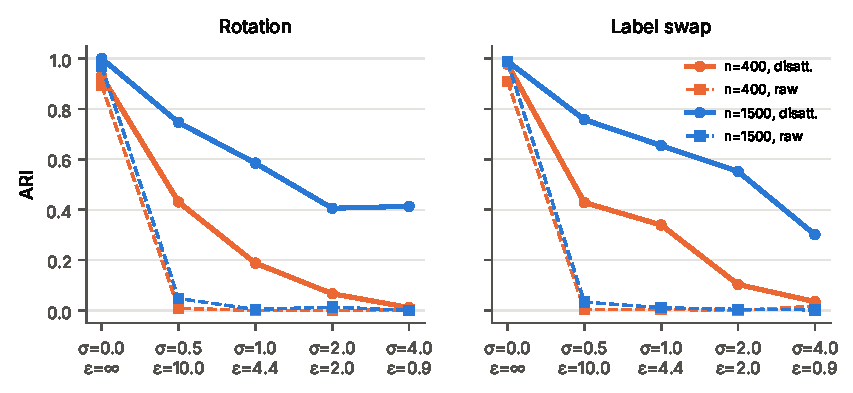
\includegraphics[width=0.85\linewidth]{dp.pdf}
\caption{Clustering quality under $(\varepsilon,10^{-5})$-DP signatures (3 seeds). Solid: DisCo-CFL; dashed: raw cosine. Orange: 400 samples per client; blue: 1{,}500.}\label{fig:dp}
\end{figure}

\paragraph{Class support.} The signatures reveal which classes a client holds (Section~\ref{sec:method}). Table~\ref{tab:support} (Appendix~\ref{app:more}) evaluates padding: under DP noise, every client also sends, for each class it does not hold, two independent noise vectors with the noise scale of its median class. Without padding the server knows the support exactly from the list of reported classes; even from the reliabilities alone ($R_i^c>0$) it would infer it with 77--92\% accuracy. With padding the list no longer reveals the support, but the reliabilities still do, with 63--84\% accuracy: a noise vector has a positive split-half correlation by chance in about 37\% of the cases, whereas a held class with enough data has a clearly positive one. Padding also costs clustering quality (ARI falls by up to $0.3$), because the noise classes add spurious evidence. It is therefore a weak mitigation. Hiding the support would need a mechanism that releases the support itself under DP, which we leave open.



\subsection{Calibration, sensitivity, ablation and cost}\label{sec:sens-cost}
\paragraph{Calibration and threshold (H3).}\label{sec:sens} Figure~\ref{fig:tau} varies $\tau$ on the clustering step. With disattenuation, ARI is $0.85$--$1.00$ for $\tau\in[0.85,0.95]$ in every concept-shift scenario, and the label-only scenario keeps $K=1$ up to $\tau=0.9$. With the raw cosine the useful range is narrower and higher thresholds over-split: at $\tau=0.95$ the label-only federation is split into 3 clusters and \emph{Rotation + QS} into 9.7 on average. Disattenuation therefore makes the threshold less sensitive towards high values, as H3 states. Towards low values the picture is reversed: at $\tau=0.8$ the raw cosine merges fewer groups than the disattenuated similarity (ARI $0.70$ against $0.60$ on \emph{Rotation}), because disattenuation raises all similarities, including those between groups. A calibrated scale thus shifts the useful range of $\tau$ upwards rather than widening it on both sides. The gain at the default threshold is moderate: without disattenuation (Table~\ref{tab:abl}) ARI drops by $0.04$--$0.11$ in the concept-shift scenarios and by $0.33$ in the label-only one. The sample-size study (Figure~\ref{fig:size} in Appendix~\ref{app:figs}) shows why. With clipped per-sample gradients, the raw cosine between clients of the same group is already $0.98$ on Fashion-MNIST, so there is little attenuation to correct; the disattenuated similarity is $0.99$--$1.00$. Attenuation becomes large under DP noise, where the raw cosine fails completely (Figure~\ref{fig:dp}). With very small clients (50--100 samples) both versions fail, for another reason: the groups become close at the reference model (between-group similarity $0.89$--$0.93$), i.e.\ the separation shrinks, and disattenuation does not help (ARI $0.13$--$0.63$, against $0.21$--$0.60$ for the raw cosine). Otsu's label-free threshold (Table~\ref{tab:diag}) lies at $0.76$--$0.83$ in the concept-shift scenarios. It recovers label swaps as well as $\tau=0.9$ (ARI $0.97$) but merges groups under rotations (ARI $0.58$--$0.71$). Over all scenarios (Table~\ref{tab:diag}) the comparison is two-sided. In the seven scenarios where DisCo-CFL fails (ARI below $0.5$), Otsu's threshold is better in four (e.g.\ Office-Home, $0.70$ against $0.26$; CIFAR-10 rotations with the pretrained network, $0.50$ against $0.07$), equal in the two SVHN scenarios and worse in one. In the 24 scenarios where DisCo-CFL succeeds it is lower in 19, equal in four and higher in one, and it splits single-concept federations (ARI $0$ in the label-only scenario). Its separation index $\eta$ does not distinguish successes from failures ($0.63$ for the $45^\circ$ rotation with ARI $1.00$, $0.73$ for CIFAR-10 label swaps with ARI $0.28$), so neither threshold dominates, and Otsu's rule does not replace $\tau$. The shrinkage $\lambda$ has almost no effect between $0.02$ and $1$ (Table~\ref{tab:lambda} in Appendix~\ref{app:figs}), including the values $0.02$ and $0.1$ that satisfy the condition of Corollary~\ref{cor:sc}.

\begin{figure}[!htbp]
\centering
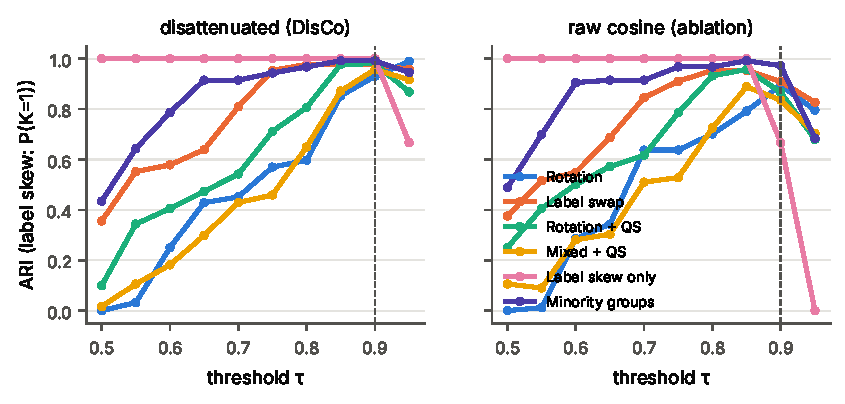
\includegraphics[width=0.85\linewidth]{tau_sensitivity.pdf}
\caption{Sensitivity to the threshold $\tau$ (3 seeds). The dashed line marks the default $\tau=0.9$, selected on the pilot runs (Section~\ref{sec:setup}).}\label{fig:tau}
\end{figure}

\paragraph{Edge cases.} The edge-case rules of Section~\ref{sec:method} were evaluated in three federations (Table~\ref{tab:edge} in Appendix~\ref{app:more}): the default minimum class size $m=4$ is best or close to best, the reliability floor $r_{\min}$ has no measurable effect, and extreme label skew ($\alpha=0.1$) or small clients lower ARI to about $0.7$.

\paragraph{Ablation (H3, H4).}
Table~\ref{tab:abl} removes one component at a time. Without class conditioning (one signature per client over all its data), clients are grouped by their label mix, the failure mode reported in the survey~\citep{benali2026survey}: 18--33 clusters and a concept accuracy 19 points lower. The mean linkage averages class-specific shifts away and merges conflicting clients (11.3\% on average, ARI $0.48$ under rotations), which supports H4: the minimum over classes matters. Linkage-ordered merging over-splits label swaps and \emph{Mixed + QS}. Without disattenuation or without clipping the federation is split more often, most visibly in the label-only scenario. Without the attachment stage, a noisy client stays alone in the label-only scenario in one of the three seeds. The table uses seeds 0--2 for all rows, so the DisCo-CFL row differs slightly from the five-seed means of Table~\ref{tab:main}. The ablation supports class conditioning and the bottleneck linkage clearly; evidence-ordered merging and clipping matter only in some scenarios (linkage-ordered merging is slightly better on \emph{Rotation}), and these two choices rest mainly on the pilot runs.

\begin{tableorg}[!htbp]
\centering
\caption{Ablation (Fashion-MNIST, 3 seeds): ARI / number of clusters $K$ per scenario, mean conflict-merge rate (\%) and mean concept accuracy (\%) over the five scenarios.}\label{tab:abl}
\scriptsize
\setlength{\tabcolsep}{3pt}
\resizebox{\textwidth}{!}{%
\begin{tabular}{lccccccc}
\toprule
Variant & Rotation & Label swap & Rot.\,+\,QS & Mixed\,+\,QS & Label only & Conflict\% & Concept \\
\midrule
DisCo-CFL (full) & 0.93 / 4.3 & 0.98 / 4.0 & 0.98 / 4.3 & 0.96 / 4.0 & 1.00 / 1.0 & 0.2 & 76.9 \\
without disattenuation (raw cosine) & 0.89 / 5.0 & 0.91 / 4.7 & 0.87 / 5.3 & 0.86 / 5.0 & 0.67 / 1.3 & 0.4 & 76.0 \\
without class conditioning & 0.05 / 31.7 & 0.04 / 32.7 & 0.03 / 33.0 & 0.02 / 29.0 & 0.00 / 17.7 & 0.8 & 57.9 \\
mean instead of bottleneck linkage & 0.48 / 3.0 & 0.70 / 4.0 & 0.79 / 4.0 & 0.58 / 4.0 & 1.00 / 1.0 & 11.3 & 73.6 \\
linkage-ordered merging & 0.95 / 4.7 & 0.85 / 5.3 & 0.97 / 4.3 & 0.77 / 6.3 & 0.67 / 1.3 & 0.0 & 75.7 \\
without per-sample clipping & 0.93 / 4.3 & 1.00 / 4.0 & 0.93 / 5.0 & 0.93 / 4.3 & 0.33 / 1.7 & 0.2 & 76.6 \\
without attachment stage & 0.91 / 5.0 & 0.98 / 4.0 & 0.97 / 4.7 & 0.96 / 4.0 & 0.67 / 1.3 & 0.1 & 76.7 \\
\bottomrule
\end{tabular}}
\end{tableorg}

\paragraph{Cost and scalability.}\label{sec:cost}
Table~\ref{tab:cost} reports wall-clock time per run and the floats each client uploads for clustering. Each DisCo-CFL client uploads its signature \emph{once}, $2p|S_i|\le2pC\approx2.0\times10^4$ floats with $p=1024$ ($1.8$--$2.0\times10^4$ on average for the default configuration in Table~\ref{tab:cost}), independent of the model dimension $d$ (46{,}730 for the small CNN, 8.4M for the ResNet-18 block). FL+HC and StoCFL upload $d$-dimensional updates or gradients for clustering, IFCA downloads $K$ models per client in every round, and FedCCFA exchanges classifiers and class anchors in every round. A DisCo-CFL run takes about as long as a FedAvg run (the times come from shared machines, so differences below about 20\% are noise; FedAvg-FT appears faster than FedAvg on the realistic benchmarks for this reason); StoCFL takes about twice as long because it trains two models per round. Computing the signature takes about 0.09\,s per client on one CPU core, and server-side clustering 0.09\,s for 40 clients and 6\,s for 320 clients. In the clustering-only scalability study, which uses 200 samples per client, ARI is $0.59$--$0.82$ for 40 to 320 clients. With 200 clients in the full pipeline (Table~\ref{tab:sweeps}) ARI is $0.88$ and accuracy is within $0.7$ points of the Oracle. The scalability study uses one seed per size and its ARI is not monotone in the number of clients, so it measures time rather than recovery.

\begin{tableorg}[!htbp]
\centering
\caption{Cost per run: mean wall-clock time (minutes; one CPU core for the small CNN, one GPU for the realistic benchmarks) and floats uploaded per client for the clustering signal. DisCo-AS: label-free warm-up (Section~\ref{sec:warmup}); DisCo-full: signature from the gradient of the whole layer-4 block (realistic benchmarks); DisCo-linkorder, DisCo-mean, DisCo-noClass, DisCo-noClip and DisCo-noDisatt: the ablation variants of Table~\ref{tab:abl} (linkage-ordered merging, mean linkage, without class conditioning, without clipping, without disattenuation).}\label{tab:cost}
\input{table_r1_cost.tex}
\end{tableorg}


\subsection{Realistic benchmarks: natural domain shift and a pretrained network}\label{sec:real}
The experiments above use small CNNs trained from scratch on images with synthetic concept groups. To test the method in a more realistic setting, we repeat the comparison with an ImageNet-pretrained ResNet-18~\citep{he2016resnet} on two datasets whose clients differ by a \emph{natural} domain shift, and on CIFAR-100.

\paragraph{Setup.} \emph{PACS}~\citep{li2017pacs} has 9{,}991 images of 7 classes in four domains (photo, art painting, cartoon, sketch). \emph{Office-Home}~\citep{venkateswara2017officehome} has 15{,}588 images of 65 classes in four domains (art, clipart, product, real world). Every domain is one concept group, with 10 clients per domain and Dirichlet label skew ($\alpha=0.3$). Clients hold 200 (PACS) or 300 (Office-Home) training images on average; \emph{PACS + QS} adds log-normal quantity skew ($\sigma=1$). \emph{CIFAR-100}~\citep{krizhevsky2009cifar} has 40 clients in four groups, either rotations ($0^\circ$--$270^\circ$) or label swaps (three groups that each swap ten random class pairs, and one group with the original labels). Images are resized to $112\times112$ ($96\times96$ for CIFAR-100). All methods train the same model, the layer-4 block and the classifier of the pretrained ResNet-18 (8.4M parameters). The earlier layers and the batch-normalisation statistics are frozen, so the layer-3 feature maps are computed once. Training uses SGD with learning rate $0.01$, batch size 64, one local epoch and 50 rounds; methods with a warm-up use 10 of them. The learning rate was chosen among $\{0.003,0.01,0.02\}$ on FedAvg, PACS, seed 0 only, in the original study, and was not re-selected for the revision. DisCo-CFL uses the gradient with respect to the final linear layer, which has a closed form, and all its other hyperparameters are unchanged. IFCA, FeSEM, FL+HC, PACFL and FedDAG-C are given the true number of groups (4); PACFL uses $16\times16$ down-sampled images. Each configuration is run with five seeds; the variants and the ablation with three. For these datasets a conflict means that two clients come from different domains (or rotation or label groups), which is stricter than necessary: two visually similar domains may well be compatible.

\begin{tableorg}[!htbp]
\centering
\caption{PACS, PACS with quantity skew, Office-Home and CIFAR-100 (40 clients, 5 seeds; DisCo-T30: 3 seeds). Columns as in Table~\ref{tab:main}; IFCA, FeSEM, FL+HC, PACFL and FedDAG-C receive the true $K=4$. The last block repeats FEMNIST (Table~\ref{tab:real_femnist}); there ARI is computed against a single group and is not meaningful.}\label{tab:real}
{\scriptsize
\resizebox{\textwidth}{!}{%
\begin{tabular}{l r c c c c c c}
\toprule
Method & n & Acc (\%) & Concept (\%) & Worst-grp (\%) & ARI & K & Conflict (\%) \\
\midrule
\multicolumn{8}{l}{\textit{PACS}} \\
DisCo & 5 & 93.3 $\pm$ 1.1 & 85.4 $\pm$ 1.7 & 90.0 $\pm$ 2.2 & 0.94 $\pm$ 0.11 & 4.0 & 1.7 \\
DisCo-noAttach & 5 & 93.3 $\pm$ 1.1 & 85.3 $\pm$ 1.6 & 90.0 $\pm$ 2.3 & 0.93 $\pm$ 0.10 & 4.2 & 1.7 \\
DisCo-T30 & 3 & 92.7 $\pm$ 3.1 & 84.6 $\pm$ 1.6 & 88.0 $\pm$ 7.6 & 0.88 $\pm$ 0.26 & 5.0 & 1.7 \\
FedAvg & 5 & 90.9 $\pm$ 1.1 & 81.3 $\pm$ 1.6 & 87.0 $\pm$ 2.3 & 0.00 $\pm$ 0.00 & 1.0 & 100.0 \\
Local & 5 & 89.7 $\pm$ 1.2 & 55.5 $\pm$ 3.1 & 84.5 $\pm$ 3.2 & 0.00 $\pm$ 0.00 & 40.0 & 0.0 \\
FedAvg-FT & 5 & 81.1 $\pm$ 3.5 & 72.2 $\pm$ 2.1 & 70.4 $\pm$ 4.7 & 0.00 $\pm$ 0.00 & 40.0 & 0.0 \\
IFCA & 5 & 91.0 $\pm$ 1.6 & 76.0 $\pm$ 3.4 & 86.8 $\pm$ 3.4 & 0.17 $\pm$ 0.12 & 4.0 & 22.5 \\
FeSEM & 5 & 91.3 $\pm$ 0.9 & 79.5 $\pm$ 1.7 & 87.7 $\pm$ 1.8 & 0.01 $\pm$ 0.04 & 4.0 & 61.8 \\
MTCFL & 5 & 91.1 $\pm$ 2.9 & 72.6 $\pm$ 2.2 & 86.4 $\pm$ 7.3 & 0.05 $\pm$ 0.03 & 25.2 & 1.1 \\
FL+HC & 5 & 91.4 $\pm$ 1.4 & 79.0 $\pm$ 1.6 & 87.2 $\pm$ 2.4 & 0.09 $\pm$ 0.13 & 4.0 & 44.2 \\
PACFL & 5 & 91.5 $\pm$ 0.8 & 81.3 $\pm$ 2.1 & 87.6 $\pm$ 3.2 & 0.30 $\pm$ 0.06 & 4.0 & 32.6 \\
StoCFL & 5 & 90.9 $\pm$ 1.1 & 72.1 $\pm$ 1.8 & 86.7 $\pm$ 3.2 & 0.07 $\pm$ 0.03 & 11.0 & 10.8 \\
StoCFL-W & 5 & 91.4 $\pm$ 1.4 & 75.8 $\pm$ 3.1 & 88.0 $\pm$ 3.1 & 0.09 $\pm$ 0.07 & 12.6 & 7.6 \\
FedCCFA & 5 & 90.0 $\pm$ 1.2 & 78.0 $\pm$ 1.0 & 85.3 $\pm$ 2.3 & 0.00 $\pm$ 0.00 & 1.0 & 100.0 \\
FedDAG-C & 5 & 90.9 $\pm$ 1.3 & 76.4 $\pm$ 3.8 & 87.2 $\pm$ 3.1 & 0.10 $\pm$ 0.16 & 4.0 & 44.2 \\
Oracle & 5 & 93.4 $\pm$ 1.1 & 85.8 $\pm$ 1.3 & 90.1 $\pm$ 2.3 & 1.00 $\pm$ 0.00 & 4.0 & 0.0 \\
\addlinespace
\multicolumn{8}{l}{\textit{PACS + QS}} \\
DisCo & 5 & 92.6 $\pm$ 0.4 & 85.6 $\pm$ 2.0 & 89.0 $\pm$ 1.0 & 0.88 $\pm$ 0.11 & 4.0 & 3.3 \\
DisCo-noAttach & 5 & 92.6 $\pm$ 0.4 & 85.6 $\pm$ 1.9 & 89.0 $\pm$ 0.9 & 0.88 $\pm$ 0.11 & 4.0 & 3.3 \\
FedAvg & 5 & 90.4 $\pm$ 0.5 & 80.1 $\pm$ 2.7 & 86.4 $\pm$ 1.5 & 0.00 $\pm$ 0.00 & 1.0 & 100.0 \\
Local & 5 & 87.1 $\pm$ 1.2 & 51.0 $\pm$ 2.5 & 81.8 $\pm$ 2.6 & 0.00 $\pm$ 0.00 & 40.0 & 0.0 \\
FedAvg-FT & 5 & 85.3 $\pm$ 1.1 & 74.6 $\pm$ 2.9 & 75.4 $\pm$ 5.3 & 0.00 $\pm$ 0.00 & 40.0 & 0.0 \\
IFCA & 5 & 90.0 $\pm$ 0.7 & 76.7 $\pm$ 3.8 & 85.5 $\pm$ 1.8 & 0.27 $\pm$ 0.23 & 4.0 & 19.5 \\
FeSEM & 5 & 89.7 $\pm$ 0.6 & 77.1 $\pm$ 3.4 & 84.6 $\pm$ 2.4 & 0.06 $\pm$ 0.05 & 4.0 & 48.2 \\
MTCFL & 5 & 90.3 $\pm$ 1.2 & 71.8 $\pm$ 2.1 & 85.3 $\pm$ 2.9 & 0.06 $\pm$ 0.01 & 25.6 & 0.9 \\
FL+HC & 5 & 89.5 $\pm$ 0.8 & 76.9 $\pm$ 3.4 & 84.4 $\pm$ 4.0 & 0.03 $\pm$ 0.03 & 4.0 & 39.0 \\
PACFL & 5 & 90.6 $\pm$ 1.0 & 79.2 $\pm$ 4.1 & 86.0 $\pm$ 3.6 & 0.45 $\pm$ 0.13 & 4.0 & 18.7 \\
StoCFL & 5 & 88.9 $\pm$ 1.4 & 68.6 $\pm$ 4.1 & 85.4 $\pm$ 1.6 & 0.05 $\pm$ 0.03 & 10.6 & 10.6 \\
StoCFL-W & 5 & 89.9 $\pm$ 1.1 & 74.5 $\pm$ 1.2 & 84.4 $\pm$ 3.9 & 0.07 $\pm$ 0.05 & 14.2 & 7.7 \\
FedCCFA & 5 & 89.9 $\pm$ 0.3 & 78.2 $\pm$ 2.6 & 85.4 $\pm$ 2.3 & 0.00 $\pm$ 0.00 & 1.2 & 99.0 \\
FedDAG-C & 5 & 89.1 $\pm$ 0.6 & 72.2 $\pm$ 3.5 & 84.7 $\pm$ 2.5 & 0.06 $\pm$ 0.07 & 4.0 & 36.9 \\
Oracle & 5 & 92.7 $\pm$ 0.5 & 85.8 $\pm$ 1.8 & 89.1 $\pm$ 0.8 & 1.00 $\pm$ 0.00 & 4.0 & 0.0 \\
\addlinespace
\multicolumn{8}{l}{\textit{Office-Home}} \\
DisCo & 5 & 69.5 $\pm$ 1.2 & 57.7 $\pm$ 2.9 & 55.4 $\pm$ 4.4 & 0.26 $\pm$ 0.16 & 3.6 & 33.6 \\
DisCo-noAttach & 5 & 69.5 $\pm$ 1.2 & 57.3 $\pm$ 3.1 & 55.5 $\pm$ 4.4 & 0.26 $\pm$ 0.16 & 4.0 & 33.1 \\
DisCo-T30 & 3 & 70.0 $\pm$ 2.6 & 59.5 $\pm$ 5.3 & 55.3 $\pm$ 4.8 & 0.41 $\pm$ 0.41 & 4.3 & 19.1 \\
FedAvg & 5 & 69.4 $\pm$ 1.5 & 58.4 $\pm$ 1.4 & 57.5 $\pm$ 3.4 & 0.00 $\pm$ 0.00 & 1.0 & 100.0 \\
Local & 5 & 61.6 $\pm$ 0.6 & 23.8 $\pm$ 1.0 & 49.1 $\pm$ 1.2 & 0.00 $\pm$ 0.00 & 40.0 & 0.0 \\
FedAvg-FT & 5 & 65.9 $\pm$ 1.7 & 55.4 $\pm$ 1.2 & 54.4 $\pm$ 2.8 & 0.00 $\pm$ 0.00 & 40.0 & 0.0 \\
IFCA & 5 & 67.6 $\pm$ 1.0 & 51.6 $\pm$ 2.0 & 55.5 $\pm$ 2.3 & 0.04 $\pm$ 0.08 & 4.0 & 29.8 \\
FeSEM & 5 & 68.7 $\pm$ 1.4 & 55.1 $\pm$ 2.0 & 56.3 $\pm$ 2.4 & 0.09 $\pm$ 0.09 & 4.0 & 34.6 \\
MTCFL & 5 & 67.6 $\pm$ 0.6 & 43.6 $\pm$ 1.2 & 55.1 $\pm$ 0.8 & 0.11 $\pm$ 0.02 & 24.2 & 0.3 \\
FL+HC & 5 & 69.8 $\pm$ 2.0 & 58.8 $\pm$ 2.7 & 54.9 $\pm$ 4.2 & 0.52 $\pm$ 0.30 & 4.0 & 22.6 \\
PACFL & 5 & 69.4 $\pm$ 2.2 & 56.1 $\pm$ 2.4 & 58.9 $\pm$ 3.7 & 0.30 $\pm$ 0.09 & 4.0 & 28.0 \\
StoCFL & 5 & 62.8 $\pm$ 0.8 & 27.4 $\pm$ 2.8 & 49.9 $\pm$ 1.4 & 0.01 $\pm$ 0.01 & 35.6 & 0.9 \\
StoCFL-W & 5 & 66.6 $\pm$ 0.6 & 34.3 $\pm$ 1.0 & 54.9 $\pm$ 1.9 & 0.00 $\pm$ 0.01 & 39.2 & 0.0 \\
FedCCFA & 5 & 67.7 $\pm$ 1.2 & 56.6 $\pm$ 1.3 & 54.5 $\pm$ 2.2 & 0.00 $\pm$ 0.00 & 1.0 & 100.0 \\
FedDAG-C & 5 & 68.1 $\pm$ 1.3 & 53.5 $\pm$ 1.3 & 53.3 $\pm$ 3.8 & 0.17 $\pm$ 0.17 & 4.0 & 35.8 \\
Oracle & 5 & 70.4 $\pm$ 1.1 & 61.5 $\pm$ 1.8 & 54.9 $\pm$ 2.9 & 1.00 $\pm$ 0.00 & 4.0 & 0.0 \\
\addlinespace
\bottomrule
\end{tabular}}
}


\end{tableorg}

\begin{tableorg}[!htbp]
\centering
\noindent\textit{Table~\ref{tab:real} (continued).}\par\smallskip
{\scriptsize
\resizebox{\textwidth}{!}{%
\begin{tabular}{l r c c c c c c}
\toprule
Method & n & Acc (\%) & Concept (\%) & Worst-grp (\%) & ARI & K & Conflict (\%) \\
\midrule
\multicolumn{8}{l}{\textit{CIFAR-100 label swaps}} \\
DisCo & 5 & 57.8 $\pm$ 0.9 & 47.4 $\pm$ 0.8 & 56.2 $\pm$ 0.4 & 0.96 $\pm$ 0.07 & 4.0 & 0.7 \\
DisCo-noAttach & 5 & 57.6 $\pm$ 0.9 & 47.0 $\pm$ 1.2 & 56.0 $\pm$ 0.6 & 0.94 $\pm$ 0.09 & 4.6 & 0.7 \\
FedAvg & 5 & 53.9 $\pm$ 0.8 & 44.5 $\pm$ 0.8 & 51.0 $\pm$ 0.6 & 0.00 $\pm$ 0.00 & 1.0 & 100.0 \\
Local & 5 & 42.0 $\pm$ 0.6 & 17.0 $\pm$ 0.2 & 40.8 $\pm$ 0.7 & 0.00 $\pm$ 0.00 & 40.0 & 0.0 \\
FedAvg-FT & 5 & 51.8 $\pm$ 0.7 & 41.1 $\pm$ 0.4 & 50.1 $\pm$ 0.9 & 0.00 $\pm$ 0.00 & 40.0 & 0.0 \\
IFCA & 5 & 49.8 $\pm$ 0.6 & 38.0 $\pm$ 1.1 & 47.5 $\pm$ 1.2 & 0.03 $\pm$ 0.07 & 4.0 & 28.9 \\
FeSEM & 5 & 52.7 $\pm$ 1.4 & 40.9 $\pm$ 1.3 & 49.9 $\pm$ 1.2 & 0.11 $\pm$ 0.11 & 4.0 & 31.8 \\
MTCFL & 5 & 51.2 $\pm$ 0.9 & 31.4 $\pm$ 1.2 & 49.6 $\pm$ 1.5 & 0.09 $\pm$ 0.03 & 25.4 & 0.4 \\
FL+HC & 5 & 55.8 $\pm$ 1.5 & 44.9 $\pm$ 1.5 & 53.1 $\pm$ 2.6 & 0.48 $\pm$ 0.20 & 4.0 & 21.1 \\
PACFL & 5 & 51.6 $\pm$ 1.0 & 40.3 $\pm$ 1.4 & 49.3 $\pm$ 1.7 & $-$0.01 $\pm$ 0.01 & 4.0 & 62.4 \\
StoCFL & 5 & 53.7 $\pm$ 0.6 & 44.0 $\pm$ 1.4 & 50.6 $\pm$ 0.9 & $-$0.00 $\pm$ 0.00 & 1.8 & 95.8 \\
StoCFL-W & 5 & 48.9 $\pm$ 0.8 & 24.4 $\pm$ 0.5 & 47.1 $\pm$ 1.2 & 0.00 $\pm$ 0.00 & 40.0 & 0.0 \\
FedCCFA & 5 & 54.8 $\pm$ 0.8 & 43.3 $\pm$ 0.8 & 52.5 $\pm$ 1.2 & $-$0.00 $\pm$ 0.01 & 11.4 & 54.3 \\
FedDAG-C & 5 & 51.7 $\pm$ 1.3 & 39.9 $\pm$ 0.8 & 48.0 $\pm$ 1.1 & 0.11 $\pm$ 0.04 & 4.0 & 31.4 \\
Oracle & 5 & 58.1 $\pm$ 0.7 & 47.8 $\pm$ 0.9 & 56.4 $\pm$ 0.7 & 1.00 $\pm$ 0.00 & 4.0 & 0.0 \\
\addlinespace
\multicolumn{8}{l}{\textit{CIFAR-100 rotations}} \\
DisCo & 5 & 51.2 $\pm$ 1.0 & 40.3 $\pm$ 1.2 & 48.5 $\pm$ 1.8 & 0.08 $\pm$ 0.07 & 2.6 & 59.7 \\
DisCo-noAttach & 5 & 51.2 $\pm$ 0.9 & 40.1 $\pm$ 1.1 & 48.4 $\pm$ 1.5 & 0.08 $\pm$ 0.07 & 3.0 & 58.9 \\
DisCo-T30 & 3 & 52.2 $\pm$ 0.9 & 41.4 $\pm$ 2.5 & 49.3 $\pm$ 2.2 & 0.01 $\pm$ 0.01 & 2.3 & 71.0 \\
FedAvg & 5 & 52.7 $\pm$ 0.5 & 42.1 $\pm$ 0.7 & 50.1 $\pm$ 1.0 & 0.00 $\pm$ 0.00 & 1.0 & 100.0 \\
Local & 5 & 37.2 $\pm$ 0.8 & 14.5 $\pm$ 0.1 & 33.8 $\pm$ 0.8 & 0.00 $\pm$ 0.00 & 40.0 & 0.0 \\
FedAvg-FT & 5 & 46.0 $\pm$ 0.9 & 37.0 $\pm$ 0.5 & 42.4 $\pm$ 0.7 & 0.00 $\pm$ 0.00 & 40.0 & 0.0 \\
IFCA & 5 & 47.8 $\pm$ 0.9 & 35.3 $\pm$ 1.1 & 44.2 $\pm$ 1.5 & 0.02 $\pm$ 0.09 & 4.0 & 29.9 \\
FeSEM & 5 & 49.0 $\pm$ 1.0 & 37.1 $\pm$ 1.2 & 45.8 $\pm$ 2.1 & 0.01 $\pm$ 0.06 & 4.0 & 30.4 \\
MTCFL & 5 & 45.1 $\pm$ 0.3 & 26.1 $\pm$ 0.8 & 41.8 $\pm$ 0.7 & 0.04 $\pm$ 0.03 & 25.6 & 1.2 \\
FL+HC & 5 & 50.4 $\pm$ 0.7 & 38.6 $\pm$ 1.2 & 47.4 $\pm$ 1.3 & 0.06 $\pm$ 0.08 & 4.0 & 44.9 \\
PACFL & 5 & 51.6 $\pm$ 0.9 & 40.3 $\pm$ 0.9 & 48.3 $\pm$ 2.4 & 0.47 $\pm$ 0.05 & 4.0 & 27.7 \\
StoCFL & 5 & 52.2 $\pm$ 0.5 & 41.2 $\pm$ 0.6 & 49.1 $\pm$ 1.6 & 0.00 $\pm$ 0.00 & 2.2 & 94.1 \\
StoCFL-W & 5 & 43.5 $\pm$ 0.5 & 20.9 $\pm$ 0.4 & 40.0 $\pm$ 0.4 & 0.00 $\pm$ 0.00 & 40.0 & 0.0 \\
FedCCFA & 5 & 49.7 $\pm$ 0.6 & 39.8 $\pm$ 0.7 & 46.1 $\pm$ 1.3 & $-$0.00 $\pm$ 0.01 & 9.8 & 60.5 \\
FedDAG-C & 5 & 49.6 $\pm$ 1.4 & 37.1 $\pm$ 1.8 & 46.4 $\pm$ 2.1 & 0.02 $\pm$ 0.01 & 4.0 & 48.9 \\
Oracle & 5 & 51.7 $\pm$ 0.4 & 41.2 $\pm$ 0.5 & 48.1 $\pm$ 0.6 & 1.00 $\pm$ 0.00 & 4.0 & 0.0 \\
\addlinespace
\multicolumn{8}{l}{\textit{FEMNIST}} \\
DisCo & 5 & 62.8 $\pm$ 0.9 & 58.6 $\pm$ 3.1 & 62.8 $\pm$ 0.9 & 0.80 $\pm$ 0.56 & 1.2 & 0.0 \\
DisCo-noAttach & 5 & 62.8 $\pm$ 0.9 & 58.6 $\pm$ 3.1 & 62.8 $\pm$ 0.9 & 0.80 $\pm$ 0.56 & 1.2 & 0.0 \\
FedAvg & 5 & 62.8 $\pm$ 0.9 & 58.7 $\pm$ 3.2 & 62.8 $\pm$ 0.9 & 1.00 $\pm$ 0.00 & 1.0 & 0.0 \\
Local & 5 & 63.6 $\pm$ 1.1 & 24.7 $\pm$ 2.1 & 63.6 $\pm$ 1.1 & 0.00 $\pm$ 0.00 & 100.0 & 0.0 \\
FedAvg-FT & 5 & 55.3 $\pm$ 0.9 & 43.5 $\pm$ 2.8 & 55.3 $\pm$ 0.9 & 0.00 $\pm$ 0.00 & 100.0 & 0.0 \\
IFCA & 5 & 65.2 $\pm$ 2.3 & 55.3 $\pm$ 5.0 & 65.2 $\pm$ 2.3 & 0.20 $\pm$ 0.56 & 2.0 & 0.0 \\
FeSEM & 5 & 64.6 $\pm$ 1.1 & 51.3 $\pm$ 4.7 & 64.6 $\pm$ 1.1 & 0.00 $\pm$ 0.00 & 3.6 & 0.0 \\
MTCFL & 5 & 63.0 $\pm$ 1.3 & 30.7 $\pm$ 2.7 & 63.0 $\pm$ 1.3 & 0.00 $\pm$ 0.00 & 65.0 & 0.0 \\
FL+HC & 5 & 63.9 $\pm$ 0.6 & 50.6 $\pm$ 4.2 & 63.9 $\pm$ 0.6 & 0.00 $\pm$ 0.00 & 4.0 & 0.0 \\
StoCFL & 5 & 62.7 $\pm$ 0.9 & 56.6 $\pm$ 4.6 & 62.7 $\pm$ 0.9 & 0.60 $\pm$ 0.68 & 1.4 & 0.0 \\
StoCFL-W & 5 & 64.5 $\pm$ 0.6 & 51.9 $\pm$ 3.6 & 64.5 $\pm$ 0.6 & 0.00 $\pm$ 0.00 & 6.0 & 0.0 \\
FedCCFA & 5 & 62.7 $\pm$ 1.3 & 53.5 $\pm$ 2.5 & 62.7 $\pm$ 1.3 & 0.40 $\pm$ 0.68 & 2.0 & 0.0 \\
FedDAG-C & 5 & 64.5 $\pm$ 0.6 & 50.7 $\pm$ 3.6 & 64.5 $\pm$ 0.6 & 0.00 $\pm$ 0.00 & 4.0 & 0.0 \\
\bottomrule
\end{tabular}}
}


\end{tableorg}

\paragraph{Where DisCo-CFL works.} On PACS (Table~\ref{tab:real}) DisCo-CFL recovers the domains in most runs (ARI $0.94\pm0.11$, 1.7\% of the conflicting pairs merged) and matches the Oracle in accuracy (93.3\% against 93.4\%), concept accuracy and worst-group accuracy. The best baselines, PACFL and FL+HC, reach 91.4--91.5\% with ARI at most $0.30$, and FedAvg 90.9\%. With quantity skew (PACS + QS) the picture is the same: 92.6\% against 92.7\% for the Oracle and 90.6\% for the best baseline (PACFL), ARI $0.88$. With label-swap groups on CIFAR-100, DisCo-CFL finds the groups without being told $K$ (ARI $0.96$, 0.7\% conflicting merges) and reaches 57.8\% (Oracle 58.1\%), against 55.8\% for FL+HC, the best baseline, and 53.9\% for FedAvg. The estimated separation is $\hat\Delta=0.21$ on PACS and $0.33$ on CIFAR-100 label swaps (Table~\ref{tab:diag}).

\paragraph{Where it does not.} On Office-Home and on rotated CIFAR-100, DisCo-CFL does not separate the groups: ARI $0.26$ and $0.08$, with 34\% and 60\% of the conflicting pairs merged. The cost in accuracy is small because there is little to gain: the Oracle improves on FedAvg by $1.0$ point on Office-Home and is $1.0$ point \emph{below} FedAvg on rotated CIFAR-100, where the pretrained features make one model sufficient. DisCo-CFL is at the level of FedAvg on Office-Home (69.5\% against 69.4\%) and $1.5$ points below it on rotated CIFAR-100 (51.2\% against 52.7\%), because it trains a few clusters with less data each. The baselines that receive the true $K$ separate these groups better but still only partly: the best ARI is $0.52$ (FL+HC) on Office-Home and $0.47$ (PACFL) on rotated CIFAR-100, and neither is more accurate than FedAvg. The diagnostics differ between the two failures. Rotated CIFAR-100 has $\hat\Delta=0.05$, below $1-\tau$: the reference model does not separate rotations of natural images, much as on CIFAR-10. Office-Home has $\hat\Delta=0.13$, just above $1-\tau=0.1$, so the margin $\gamma$ of Theorem~\ref{thm:rec} is about $0.03$ and the finite-sample condition is not met; here Otsu's label-free threshold ($0.94$) recovers more of the structure than the default (ARI $0.70$ against $0.26$, Table~\ref{tab:diag}). Table~\ref{tab:real_variants} in Appendix~\ref{app:more} reports two attempted remedies (3 seeds). A signature from the gradient of the whole layer-4 block raises ARI to $0.75$ on Office-Home and $0.32$ on rotated CIFAR-100, and a 30-round warm-up to $0.41$ and $0.01$; only the full-layer signature improves the clustering, and neither changes accuracy by more than $1.4$ points, consistent with the small gain available.



\paragraph{Ablation on CIFAR-100 label swaps.} Table~\ref{tab:real_ablation} in Appendix~\ref{app:more} removes one component at a time (3 seeds). Here every main component matters. Without class conditioning, clients are grouped by their label mix: every client is alone ($K=40$), and accuracy falls by 10 points. Without disattenuation, the 100-class signatures are noisy and the federation is split into 16 clusters (ARI $0.26$; accuracy $-7.2$ points), which supports H3 more clearly than the Fashion-MNIST ablation. With the mean instead of the bottleneck, the swaps, which touch 20 of the 100 classes, are averaged away and all groups are merged ($K=1.3$, 96\% conflicting merges; $-3.7$ points), which supports H4. Linkage-ordered merging over-splits ($K=7.7$, ARI $0.68$); clipping and attachment make little difference.



\paragraph{Statistical comparison.} Over the five realistic benchmarks, the hierarchical bootstrap gives DisCo-CFL a positive mean difference in accuracy against every baseline (Table~\ref{tab:hier}, part b), with intervals that exclude zero except against FedAvg ($+1.4$, $[-0.3,+3.1]$). With five scenarios the smallest possible Wilcoxon $p$-value is $0.031$, so these tests have little power, and the per-benchmark results above are the more informative summary: clear gains on PACS and CIFAR-100 label swaps, none on Office-Home, and a small loss on rotated CIFAR-100.

\paragraph{FEMNIST: natural writers without ground-truth groups.} FEMNIST~\citep{caldas2018leaf} has handwritten characters (62 classes) from thousands of writers. We take 100 writers with at least 150 samples and train the small CNN of the earlier experiments from scratch. There is no true number of groups, so IFCA, FeSEM, FL+HC and FedDAG-C are given $K=4$ without justification. DisCo-CFL forms one cluster in four of the five seeds and two in the fifth, and its accuracy equals that of FedAvg (62.8\%; Table~\ref{tab:real_femnist}). Methods that split the writers into a few clusters are 1.7--2.4 points more accurate on local test data (IFCA 65.2\%, FeSEM 64.6\%, FedDAG-C and StoCFL-W 64.5\%), but generalise less to other writers (pooled accuracy 50.7--55.3\% against 58.6\% for DisCo-CFL and 58.7\% for FedAvg). With a reference model of 10 rounds, the writers' class-conditional gradients are not separated enough for DisCo-CFL to split them, so on natural writer heterogeneity it reduces to FedAvg.

\begin{tableorg}[!htbp]
\centering
\caption{FEMNIST, 100 writers, 5 seeds. Pooled: accuracy on the pooled test sets of 20 writers. IFCA, FeSEM, FL+HC and FedDAG-C receive $K=4$.}\label{tab:real_femnist}
\scriptsize
\setlength{\tabcolsep}{3.5pt}
\begin{tabular}{lcccc}
\toprule
Method & Acc & Acc@10\% & Pooled & $K$ \\
\midrule
\multicolumn{5}{l}{\textit{FEMNIST (100 writers)}}\\
FedAvg & 62.8 & 47.4 & \textbf{58.7} & 1.0 \\
Local & 63.6 & 49.0 & 24.7 & 100.0 \\
FedAvg-FT & 55.3 & 31.6 & 43.5 & 100.0 \\
IFCA & \textbf{65.2} & \textbf{51.7} & 55.3 & 2.0 \\
FeSEM & 64.6 & 50.8 & 51.3 & 3.6 \\
MTCFL & 63.0 & 48.8 & 30.7 & 65.0 \\
FL+HC & 63.9 & 49.1 & 50.6 & 4.0 \\
StoCFL & 62.7 & 45.8 & 56.6 & 1.4 \\
StoCFL-W & 64.5 & 50.9 & 51.9 & 6.0 \\
FedCCFA & 62.7 & 44.3 & 53.5 & 2.0 \\
FedDAG-C & 64.5 & 50.9 & 50.7 & 4.0 \\
DisCo-noAttach & 62.8 & 47.4 & 58.6 & 1.2 \\
DisCo & 62.8 & 47.4 & 58.6 & 1.2 \\
\bottomrule
\end{tabular}

\end{tableorg}

\subsection{Additional pre-registered benchmarks}\label{sec:extra}
To test the scope stated above on data not used so far, we ran seven further scenarios whose choice and hypotheses were recorded in the repository before any of them was run (file \texttt{PREREGISTRATION\_R1\_EXTRA.md}): CIFAR-10 with the pretrained ResNet-18 of Section~\ref{sec:real}, where the small-CNN failure was attributed to an uninformative reference model; a text benchmark, AG News with a frozen sentence encoder~\citep{reimers2019sbert} and a two-layer classifier head; and KMNIST and EMNIST (47 classes) with the small CNN. Rotation and label-swap groups are built as before, all hyperparameters are unchanged, and every method was run with five seeds. The only choice made for the new data is the learning rate of the text model, which, as for PACS, was selected with FedAvg on a single-concept federation after standardising the embeddings; this amendment was recorded before any run of the compared methods. Table~\ref{tab:extra} reports all results.

\begin{tableorg}[!htbp]
\centering
\caption{Additional pre-registered benchmarks (40 clients, 5 seeds; columns as in Table~\ref{tab:main}). CIFAR-10 (ResNet): pretrained ResNet-18 as in Section~\ref{sec:real}. PACFL and FedDAG-C need image inputs and are not run on AG News.}\label{tab:extra}
{\scriptsize
\resizebox{\textwidth}{!}{%
\begin{tabular}{l r c c c c c c}
\toprule
Method & n & Acc (\%) & Concept (\%) & Worst-grp (\%) & ARI & K & Conflict (\%) \\
\midrule
\multicolumn{8}{l}{\textit{KMNIST rotation}} \\
DisCo & 5 & 86.9 $\pm$ 0.4 & 75.7 $\pm$ 2.6 & 85.0 $\pm$ 1.3 & 0.96 $\pm$ 0.07 & 4.2 & 0.7 \\
DisCo-noAttach & 5 & 86.8 $\pm$ 0.5 & 75.4 $\pm$ 2.6 & 85.0 $\pm$ 1.3 & 0.94 $\pm$ 0.08 & 4.6 & 0.7 \\
FedAvg & 5 & 74.6 $\pm$ 1.3 & 54.1 $\pm$ 2.0 & 73.0 $\pm$ 1.3 & 0.00 $\pm$ 0.00 & 1.0 & 100.0 \\
Local & 5 & 81.6 $\pm$ 0.8 & 44.4 $\pm$ 1.5 & 79.4 $\pm$ 0.8 & 0.00 $\pm$ 0.00 & 40.0 & 0.0 \\
FedAvg-FT & 5 & 76.4 $\pm$ 0.6 & 53.3 $\pm$ 2.0 & 74.9 $\pm$ 0.7 & 0.00 $\pm$ 0.00 & 40.0 & 0.0 \\
IFCA & 5 & 81.3 $\pm$ 4.2 & 61.1 $\pm$ 12.3 & 78.3 $\pm$ 4.6 & 0.43 $\pm$ 0.44 & 3.8 & 18.5 \\
FeSEM & 5 & 81.4 $\pm$ 3.5 & 61.0 $\pm$ 8.9 & 77.8 $\pm$ 1.9 & 0.34 $\pm$ 0.32 & 4.0 & 20.7 \\
MTCFL & 5 & 83.5 $\pm$ 0.8 & 56.1 $\pm$ 2.2 & 81.7 $\pm$ 1.3 & 0.13 $\pm$ 0.01 & 24.4 & 0.0 \\
FL+HC & 5 & 86.6 $\pm$ 1.1 & 74.3 $\pm$ 5.2 & 85.1 $\pm$ 1.3 & 0.89 $\pm$ 0.22 & 4.0 & 3.0 \\
PACFL & 5 & 81.1 $\pm$ 1.9 & 61.5 $\pm$ 4.0 & 78.7 $\pm$ 1.3 & 0.30 $\pm$ 0.16 & 4.0 & 26.0 \\
StoCFL & 5 & 78.3 $\pm$ 2.2 & 49.8 $\pm$ 0.4 & 75.8 $\pm$ 3.0 & 0.00 $\pm$ 0.04 & 11.4 & 9.8 \\
StoCFL-W & 5 & 80.1 $\pm$ 1.2 & 52.4 $\pm$ 1.1 & 77.4 $\pm$ 1.8 & 0.05 $\pm$ 0.05 & 14.2 & 6.2 \\
FedCCFA & 5 & 76.9 $\pm$ 1.2 & 51.7 $\pm$ 1.9 & 75.3 $\pm$ 1.7 & 0.00 $\pm$ 0.00 & 1.0 & 100.0 \\
FedDAG-C & 5 & 85.6 $\pm$ 1.9 & 72.1 $\pm$ 5.8 & 82.9 $\pm$ 3.6 & 0.76 $\pm$ 0.25 & 4.0 & 8.9 \\
Oracle & 5 & 87.2 $\pm$ 0.3 & 76.7 $\pm$ 1.2 & 85.5 $\pm$ 0.8 & 1.00 $\pm$ 0.00 & 4.0 & 0.0 \\
\addlinespace
\multicolumn{8}{l}{\textit{KMNIST label swap}} \\
DisCo & 5 & 87.3 $\pm$ 0.6 & 76.4 $\pm$ 1.3 & 86.1 $\pm$ 0.9 & 0.95 $\pm$ 0.07 & 4.2 & 0.3 \\
DisCo-noAttach & 5 & 87.3 $\pm$ 0.6 & 76.0 $\pm$ 1.0 & 86.1 $\pm$ 0.9 & 0.93 $\pm$ 0.05 & 4.6 & 0.3 \\
FedAvg & 5 & 75.6 $\pm$ 2.8 & 54.5 $\pm$ 1.2 & 68.9 $\pm$ 4.9 & 0.00 $\pm$ 0.00 & 1.0 & 100.0 \\
Local & 5 & 81.3 $\pm$ 0.9 & 44.3 $\pm$ 1.5 & 79.3 $\pm$ 0.8 & 0.00 $\pm$ 0.00 & 40.0 & 0.0 \\
FedAvg-FT & 5 & 81.6 $\pm$ 1.9 & 62.4 $\pm$ 1.2 & 79.2 $\pm$ 2.3 & 0.00 $\pm$ 0.00 & 40.0 & 0.0 \\
IFCA & 5 & 83.7 $\pm$ 1.1 & 63.2 $\pm$ 5.8 & 81.0 $\pm$ 3.4 & 0.36 $\pm$ 0.18 & 4.0 & 18.4 \\
FeSEM & 5 & 84.3 $\pm$ 2.9 & 62.8 $\pm$ 6.6 & 82.3 $\pm$ 3.8 & 0.36 $\pm$ 0.19 & 4.0 & 22.2 \\
MTCFL & 5 & 83.6 $\pm$ 1.0 & 56.4 $\pm$ 0.9 & 82.1 $\pm$ 1.3 & 0.10 $\pm$ 0.02 & 25.0 & 0.2 \\
FL+HC & 5 & 84.9 $\pm$ 0.8 & 68.0 $\pm$ 4.7 & 82.3 $\pm$ 2.8 & 0.45 $\pm$ 0.22 & 4.0 & 20.7 \\
PACFL & 5 & 76.1 $\pm$ 2.2 & 50.3 $\pm$ 1.6 & 70.0 $\pm$ 2.8 & $-$0.03 $\pm$ 0.03 & 4.0 & 36.7 \\
StoCFL & 5 & 78.6 $\pm$ 2.1 & 51.2 $\pm$ 0.7 & 73.9 $\pm$ 2.8 & 0.00 $\pm$ 0.03 & 10.8 & 9.5 \\
StoCFL-W & 5 & 82.6 $\pm$ 1.4 & 57.6 $\pm$ 1.7 & 80.2 $\pm$ 1.3 & 0.07 $\pm$ 0.06 & 15.8 & 4.7 \\
FedCCFA & 5 & 84.0 $\pm$ 1.2 & 63.2 $\pm$ 1.5 & 82.1 $\pm$ 1.6 & $-$0.00 $\pm$ 0.00 & 1.8 & 95.9 \\
FedDAG-C & 5 & 82.0 $\pm$ 2.0 & 59.8 $\pm$ 2.7 & 77.4 $\pm$ 4.5 & 0.24 $\pm$ 0.06 & 4.0 & 28.6 \\
Oracle & 5 & 87.4 $\pm$ 0.7 & 77.2 $\pm$ 0.8 & 86.0 $\pm$ 0.9 & 1.00 $\pm$ 0.00 & 4.0 & 0.0 \\
\addlinespace
\multicolumn{8}{l}{\textit{EMNIST rotation}} \\
DisCo & 5 & 84.2 $\pm$ 0.6 & 71.2 $\pm$ 1.7 & 82.8 $\pm$ 1.7 & 0.98 $\pm$ 0.04 & 4.4 & 0.0 \\
DisCo-noAttach & 5 & 83.7 $\pm$ 0.6 & 69.9 $\pm$ 1.7 & 82.3 $\pm$ 1.2 & 0.94 $\pm$ 0.04 & 5.6 & 0.0 \\
FedAvg & 5 & 65.1 $\pm$ 0.5 & 41.7 $\pm$ 1.5 & 62.9 $\pm$ 1.3 & 0.00 $\pm$ 0.00 & 1.0 & 100.0 \\
Local & 5 & 74.0 $\pm$ 0.7 & 33.0 $\pm$ 0.5 & 72.0 $\pm$ 2.1 & 0.00 $\pm$ 0.00 & 40.0 & 0.0 \\
FedAvg-FT & 5 & 69.3 $\pm$ 1.9 & 45.2 $\pm$ 1.5 & 65.1 $\pm$ 2.8 & 0.00 $\pm$ 0.00 & 40.0 & 0.0 \\
IFCA & 5 & 78.1 $\pm$ 4.9 & 58.8 $\pm$ 8.9 & 72.1 $\pm$ 8.3 & 0.59 $\pm$ 0.31 & 4.0 & 10.9 \\
FeSEM & 5 & 77.1 $\pm$ 7.5 & 58.7 $\pm$ 14.3 & 72.5 $\pm$ 8.9 & 0.54 $\pm$ 0.45 & 4.0 & 20.3 \\
MTCFL & 5 & 77.4 $\pm$ 0.5 & 46.9 $\pm$ 0.5 & 75.7 $\pm$ 1.6 & 0.13 $\pm$ 0.00 & 23.8 & 0.0 \\
FL+HC & 5 & 84.3 $\pm$ 0.4 & 71.8 $\pm$ 1.1 & 83.0 $\pm$ 0.4 & 1.00 $\pm$ 0.00 & 4.0 & 0.0 \\
PACFL & 5 & 77.4 $\pm$ 1.6 & 57.5 $\pm$ 3.5 & 75.0 $\pm$ 1.2 & 0.48 $\pm$ 0.09 & 4.0 & 16.1 \\
StoCFL & 5 & 74.0 $\pm$ 1.0 & 37.2 $\pm$ 0.9 & 71.5 $\pm$ 2.4 & 0.01 $\pm$ 0.01 & 36.2 & 0.4 \\
StoCFL-W & 5 & 75.4 $\pm$ 1.0 & 39.2 $\pm$ 1.7 & 72.5 $\pm$ 3.2 & 0.02 $\pm$ 0.01 & 37.8 & 0.0 \\
FedCCFA & 5 & 71.0 $\pm$ 1.3 & 44.7 $\pm$ 0.7 & 68.7 $\pm$ 1.2 & 0.00 $\pm$ 0.01 & 8.8 & 64.8 \\
FedDAG-C & 5 & 80.5 $\pm$ 2.7 & 64.5 $\pm$ 5.0 & 76.5 $\pm$ 4.9 & 0.72 $\pm$ 0.20 & 4.0 & 11.0 \\
Oracle & 5 & 84.4 $\pm$ 0.5 & 71.8 $\pm$ 0.9 & 83.2 $\pm$ 0.9 & 1.00 $\pm$ 0.00 & 4.0 & 0.0 \\
\addlinespace
\multicolumn{8}{l}{\textit{EMNIST label swap}} \\
DisCo & 5 & 83.7 $\pm$ 0.9 & 68.7 $\pm$ 2.1 & 82.4 $\pm$ 0.9 & 0.56 $\pm$ 0.22 & 5.6 & 2.4 \\
DisCo-noAttach & 5 & 83.5 $\pm$ 1.0 & 68.0 $\pm$ 2.3 & 82.2 $\pm$ 0.9 & 0.54 $\pm$ 0.21 & 6.4 & 2.2 \\
FedAvg & 5 & 83.0 $\pm$ 1.0 & 71.6 $\pm$ 1.2 & 80.5 $\pm$ 1.0 & 0.00 $\pm$ 0.00 & 1.0 & 100.0 \\
Local & 5 & 73.8 $\pm$ 0.7 & 33.1 $\pm$ 0.7 & 71.8 $\pm$ 2.3 & 0.00 $\pm$ 0.00 & 40.0 & 0.0 \\
FedAvg-FT & 5 & 79.1 $\pm$ 1.3 & 66.6 $\pm$ 1.0 & 76.9 $\pm$ 2.1 & 0.00 $\pm$ 0.00 & 40.0 & 0.0 \\
IFCA & 5 & 82.1 $\pm$ 0.8 & 66.8 $\pm$ 1.4 & 79.5 $\pm$ 1.1 & 0.11 $\pm$ 0.15 & 4.0 & 24.1 \\
FeSEM & 5 & 81.9 $\pm$ 0.7 & 67.5 $\pm$ 1.0 & 79.6 $\pm$ 1.6 & 0.05 $\pm$ 0.04 & 4.0 & 29.7 \\
MTCFL & 5 & 78.4 $\pm$ 0.7 & 48.2 $\pm$ 0.3 & 76.7 $\pm$ 1.9 & 0.06 $\pm$ 0.02 & 25.0 & 0.5 \\
FL+HC & 5 & 83.0 $\pm$ 1.1 & 68.4 $\pm$ 1.3 & 81.2 $\pm$ 1.8 & 0.18 $\pm$ 0.08 & 4.0 & 24.3 \\
PACFL & 5 & 81.4 $\pm$ 1.0 & 66.3 $\pm$ 1.1 & 79.2 $\pm$ 1.5 & $-$0.00 $\pm$ 0.02 & 4.0 & 35.5 \\
StoCFL & 5 & 79.0 $\pm$ 0.6 & 50.8 $\pm$ 1.0 & 77.1 $\pm$ 1.9 & 0.00 $\pm$ 0.02 & 33.8 & 0.8 \\
StoCFL-W & 5 & 79.9 $\pm$ 1.1 & 55.9 $\pm$ 1.2 & 77.4 $\pm$ 3.7 & $-$0.00 $\pm$ 0.01 & 34.4 & 0.6 \\
FedCCFA & 5 & 82.9 $\pm$ 1.0 & 70.0 $\pm$ 1.1 & 81.5 $\pm$ 1.9 & 0.00 $\pm$ 0.01 & 9.0 & 64.0 \\
FedDAG-C & 5 & 81.9 $\pm$ 0.9 & 66.7 $\pm$ 1.1 & 79.7 $\pm$ 0.9 & 0.02 $\pm$ 0.07 & 4.0 & 35.5 \\
Oracle & 5 & 84.8 $\pm$ 0.7 & 72.4 $\pm$ 1.4 & 83.6 $\pm$ 0.7 & 1.00 $\pm$ 0.00 & 4.0 & 0.0 \\
\addlinespace
\multicolumn{8}{l}{\textit{CIFAR-10 (ResNet) rotation}} \\
DisCo & 5 & 81.4 $\pm$ 1.1 & 70.4 $\pm$ 0.7 & 78.4 $\pm$ 1.8 & 0.07 $\pm$ 0.09 & 2.2 & 74.4 \\
DisCo-noAttach & 5 & 81.4 $\pm$ 1.2 & 70.3 $\pm$ 0.8 & 78.4 $\pm$ 1.8 & 0.07 $\pm$ 0.09 & 2.6 & 73.5 \\
FedAvg & 5 & 81.2 $\pm$ 1.0 & 70.3 $\pm$ 0.6 & 78.2 $\pm$ 1.8 & 0.00 $\pm$ 0.00 & 1.0 & 100.0 \\
Local & 5 & 76.2 $\pm$ 1.4 & 45.5 $\pm$ 1.6 & 72.6 $\pm$ 1.6 & 0.00 $\pm$ 0.00 & 40.0 & 0.0 \\
FedAvg-FT & 5 & 77.6 $\pm$ 1.2 & 65.9 $\pm$ 0.3 & 73.0 $\pm$ 2.0 & 0.00 $\pm$ 0.00 & 40.0 & 0.0 \\
IFCA & 5 & 80.0 $\pm$ 1.1 & 66.9 $\pm$ 0.9 & 76.5 $\pm$ 1.4 & $-$0.01 $\pm$ 0.03 & 3.4 & 39.4 \\
FeSEM & 5 & 80.2 $\pm$ 1.0 & 67.7 $\pm$ 0.8 & 77.2 $\pm$ 1.9 & $-$0.01 $\pm$ 0.02 & 4.0 & 31.5 \\
MTCFL & 5 & 79.6 $\pm$ 1.6 & 60.1 $\pm$ 0.9 & 76.2 $\pm$ 1.8 & 0.03 $\pm$ 0.02 & 24.8 & 1.5 \\
FL+HC & 5 & 80.3 $\pm$ 1.0 & 67.4 $\pm$ 0.2 & 77.7 $\pm$ 1.6 & 0.01 $\pm$ 0.06 & 4.0 & 29.9 \\
PACFL & 5 & 81.9 $\pm$ 1.2 & 70.5 $\pm$ 0.5 & 79.0 $\pm$ 1.3 & 0.42 $\pm$ 0.06 & 4.0 & 24.7 \\
StoCFL & 5 & 79.2 $\pm$ 0.6 & 62.9 $\pm$ 3.7 & 76.6 $\pm$ 0.7 & $-$0.00 $\pm$ 0.05 & 7.6 & 28.7 \\
StoCFL-W & 5 & 79.2 $\pm$ 1.4 & 63.1 $\pm$ 1.4 & 76.3 $\pm$ 1.9 & $-$0.02 $\pm$ 0.03 & 12.6 & 9.5 \\
FedCCFA & 5 & 80.3 $\pm$ 1.1 & 68.2 $\pm$ 0.6 & 76.9 $\pm$ 2.6 & 0.00 $\pm$ 0.00 & 1.0 & 100.0 \\
FedDAG-C & 5 & 80.5 $\pm$ 1.3 & 67.0 $\pm$ 0.8 & 77.1 $\pm$ 1.8 & 0.02 $\pm$ 0.03 & 4.0 & 60.6 \\
Oracle & 5 & 83.2 $\pm$ 1.3 & 73.7 $\pm$ 0.6 & 79.9 $\pm$ 1.6 & 1.00 $\pm$ 0.00 & 4.0 & 0.0 \\
\addlinespace
\multicolumn{8}{l}{\textit{CIFAR-10 (ResNet) label swap}} \\
DisCo & 5 & 88.3 $\pm$ 0.8 & 81.9 $\pm$ 0.7 & 87.0 $\pm$ 1.2 & 0.99 $\pm$ 0.04 & 4.0 & 0.2 \\
DisCo-noAttach & 5 & 88.3 $\pm$ 0.8 & 81.9 $\pm$ 0.7 & 87.0 $\pm$ 1.2 & 0.99 $\pm$ 0.04 & 4.0 & 0.2 \\
FedAvg & 5 & 71.6 $\pm$ 3.4 & 56.3 $\pm$ 0.8 & 65.2 $\pm$ 5.5 & 0.00 $\pm$ 0.00 & 1.0 & 100.0 \\
Local & 5 & 82.1 $\pm$ 1.2 & 52.5 $\pm$ 1.7 & 80.3 $\pm$ 1.2 & 0.00 $\pm$ 0.00 & 40.0 & 0.0 \\
FedAvg-FT & 5 & 83.2 $\pm$ 1.4 & 66.8 $\pm$ 2.1 & 79.9 $\pm$ 3.0 & 0.00 $\pm$ 0.00 & 40.0 & 0.0 \\
IFCA & 5 & 82.2 $\pm$ 3.8 & 68.4 $\pm$ 4.6 & 78.1 $\pm$ 4.9 & 0.45 $\pm$ 0.13 & 3.8 & 16.0 \\
FeSEM & 5 & 81.8 $\pm$ 2.5 & 66.5 $\pm$ 4.9 & 76.6 $\pm$ 5.3 & 0.34 $\pm$ 0.17 & 4.0 & 23.0 \\
MTCFL & 5 & 86.2 $\pm$ 0.9 & 71.0 $\pm$ 2.1 & 84.8 $\pm$ 1.2 & 0.11 $\pm$ 0.02 & 26.2 & 0.0 \\
FL+HC & 5 & 86.0 $\pm$ 0.7 & 75.1 $\pm$ 3.7 & 83.6 $\pm$ 1.9 & 0.64 $\pm$ 0.19 & 4.0 & 13.2 \\
PACFL & 5 & 72.3 $\pm$ 2.7 & 54.8 $\pm$ 1.4 & 67.4 $\pm$ 4.4 & $-$0.01 $\pm$ 0.02 & 4.0 & 53.9 \\
StoCFL & 5 & 75.0 $\pm$ 4.3 & 54.7 $\pm$ 3.7 & 70.4 $\pm$ 5.2 & 0.02 $\pm$ 0.03 & 9.0 & 21.8 \\
StoCFL-W & 5 & 84.2 $\pm$ 0.9 & 65.9 $\pm$ 1.2 & 82.6 $\pm$ 1.0 & 0.12 $\pm$ 0.05 & 21.0 & 2.1 \\
FedCCFA & 5 & 85.3 $\pm$ 1.2 & 69.1 $\pm$ 1.5 & 83.2 $\pm$ 1.7 & 0.00 $\pm$ 0.00 & 1.0 & 100.0 \\
FedDAG-C & 5 & 73.8 $\pm$ 4.1 & 57.0 $\pm$ 3.5 & 67.1 $\pm$ 7.1 & 0.03 $\pm$ 0.06 & 4.0 & 67.9 \\
Oracle & 5 & 88.3 $\pm$ 0.8 & 82.0 $\pm$ 0.4 & 87.0 $\pm$ 1.2 & 1.00 $\pm$ 0.00 & 4.0 & 0.0 \\
\addlinespace
\multicolumn{8}{l}{\textit{AG News label swap}} \\
DisCo & 5 & 89.4 $\pm$ 3.2 & 81.5 $\pm$ 5.8 & 84.8 $\pm$ 8.3 & 0.79 $\pm$ 0.21 & 3.4 & 10.5 \\
DisCo-noAttach & 5 & 89.5 $\pm$ 3.1 & 81.5 $\pm$ 5.8 & 85.0 $\pm$ 8.0 & 0.79 $\pm$ 0.21 & 3.6 & 10.2 \\
FedAvg & 5 & 75.2 $\pm$ 6.7 & 55.1 $\pm$ 1.8 & 67.7 $\pm$ 10.5 & 0.00 $\pm$ 0.00 & 1.0 & 100.0 \\
Local & 5 & 89.6 $\pm$ 1.0 & 77.4 $\pm$ 0.8 & 87.9 $\pm$ 2.5 & 0.00 $\pm$ 0.00 & 40.0 & 0.0 \\
FedAvg-FT & 5 & 89.5 $\pm$ 1.0 & 68.1 $\pm$ 2.1 & 87.5 $\pm$ 3.6 & 0.00 $\pm$ 0.00 & 40.0 & 0.0 \\
IFCA & 5 & 87.6 $\pm$ 4.5 & 73.7 $\pm$ 13.3 & 83.4 $\pm$ 6.7 & 0.53 $\pm$ 0.32 & 4.0 & 12.4 \\
FeSEM & 5 & 85.4 $\pm$ 4.7 & 66.9 $\pm$ 7.3 & 81.5 $\pm$ 7.4 & 0.24 $\pm$ 0.14 & 4.0 & 25.5 \\
MTCFL & 5 & 90.5 $\pm$ 0.9 & 81.1 $\pm$ 1.5 & 88.9 $\pm$ 2.6 & 0.11 $\pm$ 0.01 & 24.8 & 0.2 \\
FL+HC & 5 & 87.8 $\pm$ 2.5 & 72.7 $\pm$ 4.1 & 85.2 $\pm$ 3.6 & 0.37 $\pm$ 0.09 & 4.0 & 18.6 \\
StoCFL & 5 & 84.2 $\pm$ 2.7 & 64.6 $\pm$ 6.9 & 79.6 $\pm$ 6.3 & 0.11 $\pm$ 0.15 & 6.2 & 16.9 \\
StoCFL-W & 5 & 89.2 $\pm$ 1.6 & 75.7 $\pm$ 6.6 & 86.9 $\pm$ 3.2 & 0.29 $\pm$ 0.16 & 8.6 & 7.9 \\
FedCCFA & 5 & 90.6 $\pm$ 0.9 & 72.4 $\pm$ 3.1 & 88.7 $\pm$ 3.0 & 0.39 $\pm$ 0.35 & 2.6 & 46.3 \\
Oracle & 5 & 91.6 $\pm$ 0.8 & 87.1 $\pm$ 0.5 & 90.2 $\pm$ 2.0 & 1.00 $\pm$ 0.00 & 4.0 & 0.0 \\
\bottomrule
\end{tabular}}
}

\end{tableorg}

\paragraph{Outcomes of the pre-registered hypotheses.} Three of the four predictions of success hold, and the predicted failure occurs. (i) On CIFAR-10 with label swaps and the pretrained network, DisCo-CFL recovers the groups (ARI $0.99$, $\hat\Delta=0.34$) and equals the oracle (88.3\%), against 86.2\% for the best baseline (MTCFL); the best baseline ARI is $0.64$ (FL+HC, given $K$). This confirms the diagnosis of the small-CNN failure on CIFAR-10: with an informative reference model the same label-swap groups are recovered. (ii) On CIFAR-10 rotations the pretrained features do not separate the groups ($\hat\Delta=0.02$) and DisCo-CFL fails (ARI $0.07$), as predicted from rotated CIFAR-100; its accuracy is 0.5 points below the best baseline (PACFL, given $K$). (iii) On KMNIST (rotations and label swaps) and EMNIST rotations, DisCo-CFL recovers the groups (ARI $0.95$--$0.98$) and is within $0.3$ points of the oracle. (iv) Two predictions fail. On EMNIST label swaps ARI is $0.56$: the groups are separated ($\hat\Delta=0.32$), but with 47 classes the per-class signatures are noisy, the smallest pooled linkage within a true group is $0.88<\tau$, and DisCo-CFL over-splits (5.6 clusters, 2.2\% of the conflicting pairs merged). Its accuracy (83.7\%) is still the highest among non-oracle methods, 1.1 points below the oracle. On AG News ARI is $0.79$, just below the pre-registered $0.8$; the separation is small ($\hat\Delta=0.13$, as on Office-Home), and in three of the five seeds two groups are merged into one ($K=3$, ARI $0.62$--$0.70$), while the other two seeds recover the groups (ARI $0.93$ and $1.00$). DisCo-CFL is 2.2 points below the oracle in accuracy; FedCCFA has a higher local accuracy (90.6\% against 89.4\%) but a 9-point lower concept accuracy.

\paragraph{Summary.} Across the seven scenarios the hierarchical comparison gives DisCo-CFL a higher mean accuracy than every baseline, with intervals that exclude zero ($+1.2$ points against FL+HC, the closest, to $+10.7$ against FedAvg; Table~\ref{tab:hier}, part c), and a higher concept accuracy by $4.0$--$27.9$ points. Its failure rate is 23\%, against 54--100\% for the baselines (Table~\ref{tab:failure}). The outcomes follow the separation diagnostic of Section~\ref{sec:theory}: recovery succeeds where $\hat\Delta\ge0.24$ and the within-group linkage stays above $\tau$, and fails where $\hat\Delta$ is near or below $1-\tau$ or where noisy signatures with many classes push the within-group linkage below $\tau$.

\subsection{When does DisCo-CFL succeed? Separation and the theory}\label{sec:sep}
\paragraph{Separation predicts success.} Figure~\ref{fig:separation} puts together all 31 scenarios with more than one group, from every benchmark. The estimated separation $\hat\Delta$ and the ARI of DisCo-CFL are strongly associated (Spearman $\rho=0.81$ over scenario means), and the rule ``$\hat\Delta>1-\tau$'' that Theorem~\ref{thm:rec} suggests classifies the scenarios into successes (ARI $\ge0.5$) and failures correctly in 29 of 31 cases, and in 27 of 31 at the stricter recovery level ARI $\ge0.8$ used in the hypotheses of Section~\ref{sec:extra} (there the exceptions are Office-Home, EMNIST label swaps, AG News and the 8-permutation sweep, all with $\hat\Delta>1-\tau$). We give no $p$-value: the scenarios share datasets and models and are not independent, and the association is partly mechanical, because $\hat\Delta$ is computed from the same pooled linkage that the clustering thresholds at $\tau$, which was itself chosen on four of these scenarios. The two exceptions are borderline: the $15^\circ$ rotation ($\hat\Delta=0.06$, ARI $0.52$) and Office-Home ($\hat\Delta=0.13$, ARI $0.26$). EMNIST label swaps, the one scenario where a clearly separated group is split, are counted as a success at ARI $0.56$. The failures of DisCo-CFL are therefore not erratic: they occur where the condition of the theory does not hold. The diagnostic needs the true groups and is computed after the fact; it explains the results but does not choose the reference model in advance (Section~\ref{sec:warmup}).

\begin{figure}[!htbp]
\centering
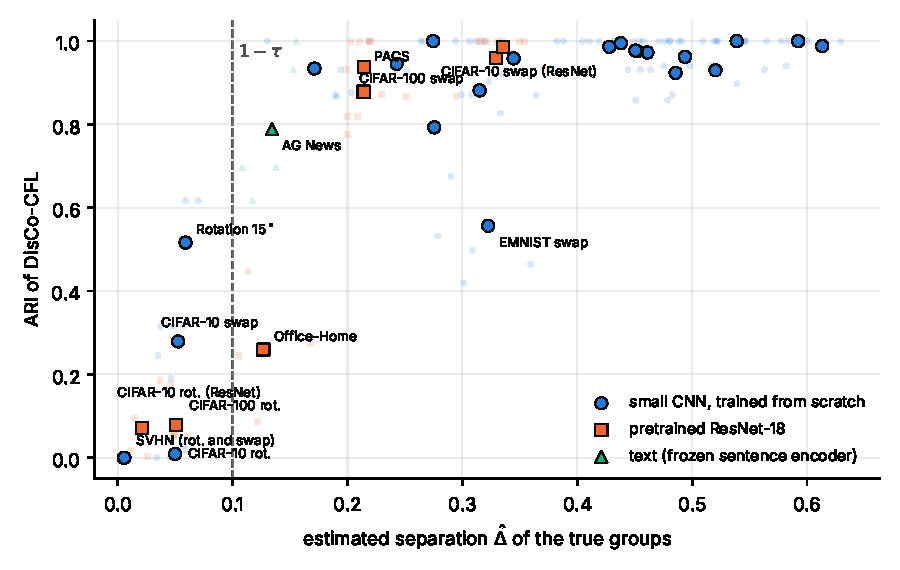
\includegraphics[width=0.85\linewidth]{separation.pdf}
\caption{ARI of DisCo-CFL against the estimated separation $\hat\Delta$ of the true groups, for all 31 scenarios with more than one group (large markers: means over seeds; small markers: individual runs). The dashed line is $1-\tau$, the separation that Theorem~\ref{thm:rec} requires.}\label{fig:separation}
\end{figure}


\paragraph{The results under the shrinkage covered by the theory.} The evidence condition of Theorem~\ref{thm:rec} cannot hold at the default shrinkage $\lambda=0.5$, but it can at $\lambda=0.02$ (Remark~\ref{rem:scope}(e)). We therefore reran the complete pipeline (warm-up, clustering, cluster training and evaluation) with $\lambda=0.02$ on all 24 small-CNN scenarios, with the predictions that accuracy changes by at most $0.5$ points wherever the default recovers the groups and that ARI changes by at most $0.05$ on average (Table~\ref{tab:l02} in Appendix~\ref{app:more}). Both hold. Where the default recovers the groups, mean accuracy changes by $-0.3$ to $+0.2$ points, and over all scenarios the mean absolute change in ARI is $0.014$; the largest changes are on the $15^\circ$ rotation (ARI $0.52\to0.44$) and \emph{Rotation + QS} ($0.99\to0.94$). The classification of the scenarios into successes and failures is the same under the shrinkage that the theorem covers, except for the borderline $15^\circ$ rotation, which falls from ARI $0.52$ to $0.44$; at the stricter level ARI $\ge0.8$, the 8-permutation sweep moves from $0.79$ to $0.81$.

\paragraph{Synthetic signatures.} On synthetic signatures with known ground truth the disattenuated similarity is nearly unbiased, whereas the raw cosine is biased by up to $-0.37$, and the guarantees of Theorem~\ref{thm:rec} are reached once $h\ge64$ (Figure~\ref{fig:theory} in Appendix~\ref{app:more}).

\subsection{Choosing the warm-up without labels}\label{sec:warmup}
The failures on SVHN and CIFAR-10 come from a reference model that has not yet learned the task (Section~\ref{sec:datasets}), and 30 warm-up rounds repair SVHN label swaps. The separation diagnostic needs the true groups, however, so it cannot choose the warm-up length in practice. A first rule that stopped the warm-up when the training loss reached a plateau failed on SVHN (on one seed), because the loss is also flat \emph{before} learning starts. We therefore designed a second rule from two principles, with round constants that were not tuned. The rule, DisCo-AS, checks the federation after 10, 15, 20, 25 and 30 rounds of FedAvg and stops at the first checkpoint where (i) the training loss of the global model, reported by the clients as one scalar each, is at most $0.75\log C$ at this and at the previous checkpoint, i.e.\ the model has clearly learned something, and (ii) the DisCo-CFL partitions computed at the two checkpoints agree (ARI between them at least $0.9$); otherwise it stops at 30 rounds. No group labels are used. The predictions were that DisCo-AS changes accuracy by at most $0.5$ points where the default works (H-AS1) and improves both ARI and accuracy on SVHN and CIFAR-10 (H-AS2).

Table~\ref{tab:as} compares the rule with the default on all small-CNN scenarios, and both predictions hold. In the eleven scenarios of Fashion-MNIST, MNIST, KMNIST and EMNIST rotations where the default works, DisCo-AS stops after 15--25 rounds and changes accuracy by $-0.4$ to $+0.1$ points; the largest drop in ARI is from $0.98$ to $0.95$ on EMNIST rotations. On SVHN and CIFAR-10 it detects that the model has not yet learned and uses the full 30 rounds in every run, so there it coincides with DisCo-T30 (Table~\ref{tab:other}); its contribution is to make this choice without labels, not a better warm-up than 30 fixed rounds. It improves both ARI and accuracy in all four scenarios: by $11.9$ points (ARI $0.81$) on SVHN label swaps, which it now recovers in most runs, by $4.0$ points on SVHN rotations, and by $0.4$--$0.7$ points on CIFAR-10, where 30 rounds remain too few. The rule thus removes the main practical failure of the fixed warm-up on SVHN label swaps, but within a 50-round budget it cannot help when the model needs longer to separate the groups. It has been evaluated only on the small-CNN scenarios.

\begin{table}[!htbp]
\centering
\caption{Fixed 10-round warm-up (DisCo) against the label-free stable warm-up (DisCo-AS), on all small-CNN scenarios (5 seeds; sweeps 3 seeds). $\Delta$: difference in mean accuracy (points). $T_0$: warm-up length chosen by DisCo-AS. FMNIST: Fashion-MNIST; QS: quantity skew; part.: participation.}\label{tab:as}
\scriptsize
\setlength{\tabcolsep}{3pt}
\begin{tabular}{lrcccccc}
\toprule
 & & \multicolumn{3}{c}{Accuracy (\%)} & \multicolumn{2}{c}{ARI} & \\
\cmidrule(lr){3-5}\cmidrule(lr){6-7}
Scenario & $n$ & DisCo & DisCo-AS & $\Delta$ & DisCo & DisCo-AS & $T_0$ chosen (range) \\
\midrule
FMNIST rotation & 5 & 89.1 & 89.0 & -0.1 & 0.92 & 0.93 & 15 (15--15) \\
FMNIST label swap & 5 & 89.2 & 89.2 & -0.0 & 0.97 & 0.97 & 15 (15--15) \\
FMNIST rotation + QS & 5 & 88.9 & 88.8 & -0.1 & 0.99 & 0.98 & 15 (15--15) \\
FMNIST mixed + QS & 5 & 89.0 & 89.1 & +0.1 & 0.96 & 0.96 & 15 (15--15) \\
FMNIST label skew only & 5 & 94.5 & 94.5 & -0.0 & 1.00 & 1.00 & 15 (15--15) \\
FMNIST minority & 5 & 89.2 & 89.2 & -0.0 & 0.99 & 1.00 & 15 (15--15) \\
MNIST rotation & 5 & 98.1 & 98.1 & +0.0 & 1.00 & 1.00 & 15 (15--15) \\
MNIST label swap & 5 & 98.0 & 98.0 & +0.0 & 0.99 & 0.99 & 15 (15--15) \\
KMNIST rotation & 5 & 86.9 & 87.0 & +0.1 & 0.96 & 0.98 & 17 (15--20) \\
KMNIST label swap & 5 & 87.3 & 87.4 & +0.1 & 0.95 & 0.99 & 16 (15--20) \\
EMNIST rotation & 5 & 84.2 & 83.7 & -0.4 & 0.98 & 0.95 & 21 (20--25) \\
EMNIST label swap & 5 & 83.7 & 84.6 & +1.0 & 0.56 & 0.65 & 22 (15--30) \\
SVHN rotation & 5 & 69.3 & 73.3 & +4.0 & 0.00 & 0.27 & 30 (30--30) \\
SVHN label swap & 5 & 73.3 & 85.1 & +11.9 & 0.00 & 0.81 & 30 (30--30) \\
CIFAR-10 rotation & 5 & 63.5 & 63.9 & +0.4 & 0.01 & 0.10 & 30 (30--30) \\
CIFAR-10 label swap & 5 & 65.3 & 65.9 & +0.7 & 0.28 & 0.37 & 30 (30--30) \\
Rotation $15^\circ$ & 3 & 88.7 & 88.6 & -0.1 & 0.52 & 0.54 & 20 (15--30) \\
Rotation $30^\circ$ & 3 & 88.8 & 88.9 & +0.0 & 0.93 & 0.98 & 17 (15--20) \\
Rotation $45^\circ$ & 3 & 89.1 & 89.1 & -0.1 & 1.00 & 1.00 & 15 (15--15) \\
2 label permutations & 3 & 89.5 & 89.5 & -0.0 & 1.00 & 1.00 & 15 (15--15) \\
8 label permutations & 3 & 88.2 & 88.2 & +0.0 & 0.79 & 0.82 & 18 (15--25) \\
Rotation, 30\% part. & 3 & 87.1 & 86.9 & -0.2 & 0.93 & 0.93 & 15 (15--15) \\
Label swap, 30\% part. & 3 & 87.3 & 87.2 & -0.1 & 0.98 & 0.98 & 15 (15--15) \\
Rotation, 200 clients & 3 & 86.5 & 86.6 & +0.1 & 0.88 & 0.93 & 20 (20--20) \\
\bottomrule
\end{tabular}

\end{table}

\subsection{Beyond accuracy: transparency, accountability, robustness and privacy}\label{sec:fat-exp}
\paragraph{Transparency: explanations and diagnosis (H5).}
Table~\ref{tab:fat} evaluates the class-level explanations against the ground truth. For label-swap groups the divergent classes reported by the server are \emph{exactly} the swapped classes in every pair of clusters (precision, recall and exact match $1.00$), and the diagnosis ``class-specific concept shift'' is always correct. A typical explanation reads: \emph{``cluster 0 vs.\ cluster 2: class-specific concept shift on classes [4, 5, 6, 7]''}, where group 2 swaps $4\leftrightarrow5$ and $6\leftrightarrow7$. For rotations, precision is again $1.00$: no class is reported as divergent when it is not. Recall is lower ($0.75$ for rotations, $0.78$ for \emph{Mixed + QS}). The misses are classes on which the two concepts are close at the reference model, such as nearly symmetric items under a $180^\circ$ rotation. Proposition~\ref{prop:expl} guarantees fidelity only for classes with enough pooled evidence and a separation $\Delta$, so these misses are within its scope, but they make the diagnosis ``global shift'' correct for only 43\% of the rotation pairs.

\begin{table}[!htbp]
\centering
\caption{Transparency and accountability (Fashion-MNIST, 3 seeds, default settings). Certificates: share of clients with a confident certificate, and share of correctly placed clients (no conflict with any member of their cluster) among confident and among uncertain certificates.}\label{tab:fat}
\small
\begin{tabular}{lccc}
\toprule
& Rotation & Label swap & Mixed + QS \\
\midrule
\multicolumn{4}{l}{\emph{Explanations: divergent classes between clusters}}\\
precision & 1.00 & 1.00 & 1.00 \\
recall & 0.75 & 1.00 & 0.78 \\
exact set / diagnosis correct & 0.43 & 1.00 & 0.33 \\
\midrule
\multicolumn{4}{l}{\emph{Certificates}}\\
share of confident certificates & 0.76 & 0.87 & 0.77 \\
correct among confident & 0.923 & 1.000 & 1.000 \\
correct among uncertain & 0.690 & 1.000 & 1.000 \\
\midrule
\multicolumn{4}{l}{\emph{Newcomers}}\\
known concept, correctly assigned & 0.96 & 0.96 & -- \\
novel concept, flagged as novel & 1.00 & 1.00 & -- \\
\bottomrule
\end{tabular}
\end{table}

\paragraph{Accountability: certificates, audit log, newcomers (H5).}
With the jackknife standard errors of Eq.~\eqref{eq:cert}, 76--87\% of the clients receive a confident certificate. Confident certificates are correct in all cases for label swaps and \emph{Mixed + QS}, and in 92.3\% of the cases for rotations, against 69.0\% for uncertain ones. Where every client is correctly placed, the uncertain certificates are therefore conservative, as the simulation of Section~\ref{sec:outputs} predicts; under rotations they do point to the clients whose placement is in doubt. A confident certificate is informative but not a guarantee, and we report it as an empirical rate, not as a coverage probability. In an exploratory analysis on the other small-CNN datasets (Table~\ref{tab:cert_ext} in Appendix~\ref{app:more}; 3 seeds), the same holds where the clustering works: on MNIST, KMNIST and EMNIST, 91--100\% of the confident certificates are correct. Where the reference model does not separate the groups, however, the certificates do not reveal the failure. On SVHN every client is placed in one cluster with a confident certificate, and every such certificate is wrong; on CIFAR-10 only 2--33\% of the confident certificates are correct. A certificate measures how well a client fits its cluster at the given reference model; it cannot detect that the reference model itself does not separate the concepts, which is the failure mode that the warm-up rule of Section~\ref{sec:warmup} addresses. Newcomers that join after clustering, using the frozen reference model, are assigned to the right cluster in 96\% of the cases, and clients with a concept never seen during clustering are reported as \emph{novel} in all cases.

\paragraph{Dependence on the reference model.} The reference model is trained on the clients that are then clustered. To test whether the partition depends on which clients trained it, we trained it on a random half of the clients, or on all clients except those of one concept group, and clustered all clients at that model (Table~\ref{tab:refmodel} in Appendix~\ref{app:more}; six Fashion-MNIST and MNIST scenarios, 3 seeds). We predicted that ARI would change by at most $0.05$ with a random half and that at most 5\% of the conflicting pairs involving an excluded group would be merged; both hold. With a random half, ARI changes by at most $0.05$ against the full reference model, and the label-only federation stays a single cluster; clients that did not train the model are placed slightly less well than those that did (ARI $0.91$--$1.00$ against $1.00$). A group that never contributed to the reference model is still separated: at most $1.1\%$ of the conflicting pairs that involve it are merged. In these scenarios the clustering does not hinge on which clients trained the reference model, as long as the model has learned the task; this does not extend to the datasets where it has not (Sections~\ref{sec:datasets} and~\ref{sec:warmup}).

\paragraph{Concept drift after clustering.} We tested the following drift procedure: after clustering, 10\% or 20\% of the clients switch to another concept group, the server recomputes all signatures at the same reference model, and every client whose similarity to its own cluster falls below $\tau$ is flagged (Table~\ref{tab:drift} in Appendix~\ref{app:more}). Every drifted client is detected (detection rate $1.00$ in all settings), but the predicted rate of at most 5\% false alarms is \emph{not} met: 31--67\% of the unchanged clients are also flagged, and 38--75\% of the drifted clients are reassigned to the cluster of their new group. The cause is that the drifted clients remain members of their old cluster and pull the bottleneck similarity of their former cluster-mates below $\tau$. In an exploratory analysis, computing each client's similarity only to the members that did not drift (in practice, members that kept a confident certificate) reduces the false-alarm rate to 1--4\% with detection unchanged. Drift detection therefore works, but needs an iterative rule that first removes the clients that changed.



\paragraph{Malicious clients.} DisCo-CFL has no defence against adversarial clients, and we measured what happens when $m\in\{1,2,4\}$ of 40 clients send manipulated signatures (Table~\ref{tab:byz} in Appendix~\ref{app:more}; no hypothesis was made). Random vectors have no split-half reliability and are flagged as low-evidence or anomalous in every run; sign-flipped signatures are isolated, alone or among themselves. Neither attack harms the clustering of the honest clients (ARI $0.95$--$0.96$, at most 0.4\% conflicting merges, as without attack). A client that copies the signature of an honest client from another group, however, is always merged into that group, without being flagged: the signature carries no information that could reveal the copy. Defending against such mimicry would need authentication of the signature or secure aggregation of the clustering step, which we leave open; Byzantine-robust aggregation~\citep{dang2026fortress} protects the training of the cluster models, not the clustering signal.



\paragraph{Privacy.}
Figure~\ref{fig:dp} shows the ARI of the clustering when the signatures are released with the Gaussian mechanism of Proposition~\ref{prop:dp} ($C_{\rm clip}=0.5$, $\delta=10^{-5}$). These results measure the utility cost of noising the clustering signal only; the warm-up and the cluster training are not private (Remark~\ref{rem:dp}). As Proposition~\ref{prop:dp}(iii) predicts, the \emph{raw} cosine collapses to ARI $\approx0$ at every noise level, with 22--40 clusters: the noise attenuates all similarities. With disattenuation the clustering degrades gradually, and more data per client buys more privacy, as the $h\propto\sigma_{\rm dp}$ term predicts. Recovery is only partial, however. With 1{,}500 samples per client, ARI is $0.75$ and $0.76$ (rotation and label swap) at $\varepsilon=10$, $0.58$ and $0.65$ at $\varepsilon=4.4$, and $0.41$ and $0.55$ at $\varepsilon=2$; with 400 samples it is at most $0.43$ at any noise level we tried. Strong privacy for the clustering signal therefore needs much larger clients than our benchmarks have.

\begin{figure}[!htbp]
\centering
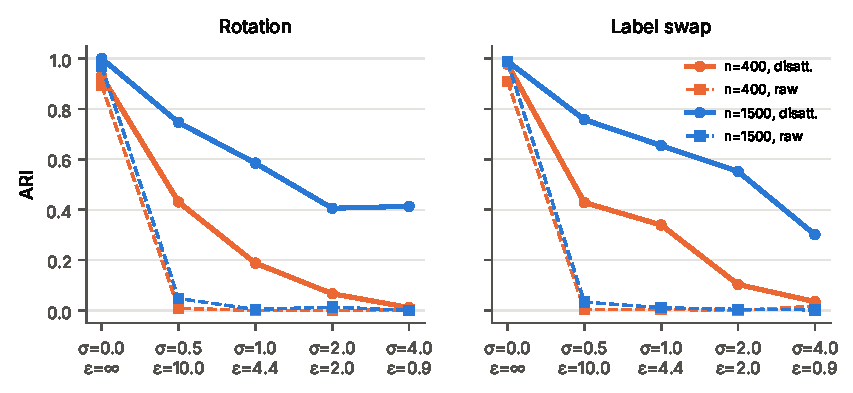
\includegraphics[width=0.85\linewidth]{dp.pdf}
\caption{Clustering quality under $(\varepsilon,10^{-5})$-DP signatures (3 seeds). Solid: DisCo-CFL; dashed: raw cosine. Orange: 400 samples per client; blue: 1{,}500.}\label{fig:dp}
\end{figure}

\paragraph{Class support.} The signatures reveal which classes a client holds (Section~\ref{sec:method}). Table~\ref{tab:support} (Appendix~\ref{app:more}) evaluates padding: under DP noise, every client also sends, for each class it does not hold, two independent noise vectors with the noise scale of its median class. Without padding the server knows the support exactly from the list of reported classes; even from the reliabilities alone ($R_i^c>0$) it would infer it with 77--92\% accuracy. With padding the list no longer reveals the support, but the reliabilities still do, with 63--84\% accuracy: a noise vector has a positive split-half correlation by chance in about 37\% of the cases, whereas a held class with enough data has a clearly positive one. Padding also costs clustering quality (ARI falls by up to $0.3$), because the noise classes add spurious evidence. It is therefore a weak mitigation. Hiding the support would need a mechanism that releases the support itself under DP, which we leave open.



\subsection{Calibration, sensitivity, ablation and cost}\label{sec:sens-cost}
\paragraph{Calibration and threshold (H3).}\label{sec:sens} Figure~\ref{fig:tau} varies $\tau$ on the clustering step. With disattenuation, ARI is $0.85$--$1.00$ for $\tau\in[0.85,0.95]$ in every concept-shift scenario, and the label-only scenario keeps $K=1$ up to $\tau=0.9$. With the raw cosine the useful range is narrower and higher thresholds over-split: at $\tau=0.95$ the label-only federation is split into 3 clusters and \emph{Rotation + QS} into 9.7 on average. Disattenuation therefore makes the threshold less sensitive towards high values, as H3 states. Towards low values the picture is reversed: at $\tau=0.8$ the raw cosine merges fewer groups than the disattenuated similarity (ARI $0.70$ against $0.60$ on \emph{Rotation}), because disattenuation raises all similarities, including those between groups. A calibrated scale thus shifts the useful range of $\tau$ upwards rather than widening it on both sides. The gain at the default threshold is moderate: without disattenuation (Table~\ref{tab:abl}) ARI drops by $0.04$--$0.11$ in the concept-shift scenarios and by $0.33$ in the label-only one. The sample-size study (Figure~\ref{fig:size} in Appendix~\ref{app:figs}) shows why. With clipped per-sample gradients, the raw cosine between clients of the same group is already $0.98$ on Fashion-MNIST, so there is little attenuation to correct; the disattenuated similarity is $0.99$--$1.00$. Attenuation becomes large under DP noise, where the raw cosine fails completely (Figure~\ref{fig:dp}). With very small clients (50--100 samples) both versions fail, for another reason: the groups become close at the reference model (between-group similarity $0.89$--$0.93$), i.e.\ the separation shrinks, and disattenuation does not help (ARI $0.13$--$0.63$, against $0.21$--$0.60$ for the raw cosine). Otsu's label-free threshold (Table~\ref{tab:diag}) lies at $0.76$--$0.83$ in the concept-shift scenarios. It recovers label swaps as well as $\tau=0.9$ (ARI $0.97$) but merges groups under rotations (ARI $0.58$--$0.71$). Over all scenarios (Table~\ref{tab:diag}) the comparison is two-sided. In the seven scenarios where DisCo-CFL fails (ARI below $0.5$), Otsu's threshold is better in four (e.g.\ Office-Home, $0.70$ against $0.26$; CIFAR-10 rotations with the pretrained network, $0.50$ against $0.07$), equal in the two SVHN scenarios and worse in one. In the 24 scenarios where DisCo-CFL succeeds it is lower in 19, equal in four and higher in one, and it splits single-concept federations (ARI $0$ in the label-only scenario). Its separation index $\eta$ does not distinguish successes from failures ($0.63$ for the $45^\circ$ rotation with ARI $1.00$, $0.73$ for CIFAR-10 label swaps with ARI $0.28$), so neither threshold dominates, and Otsu's rule does not replace $\tau$. The shrinkage $\lambda$ has almost no effect between $0.02$ and $1$ (Table~\ref{tab:lambda} in Appendix~\ref{app:figs}), including the values $0.02$ and $0.1$ that satisfy the condition of Corollary~\ref{cor:sc}.

\begin{figure}[!htbp]
\centering
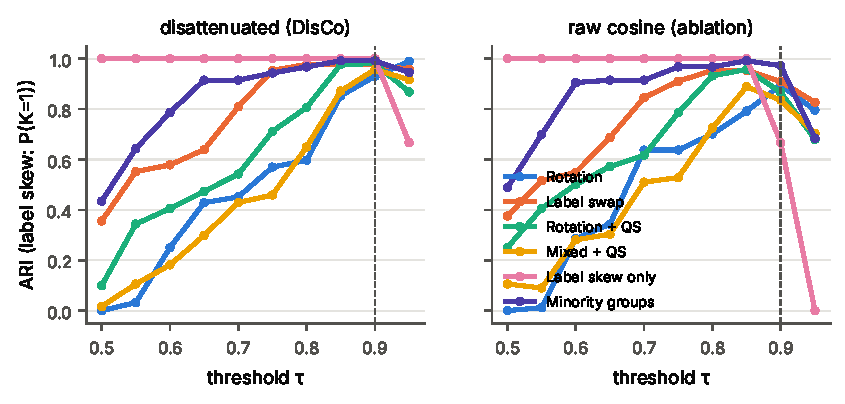
\includegraphics[width=0.85\linewidth]{tau_sensitivity.pdf}
\caption{Sensitivity to the threshold $\tau$ (3 seeds). The dashed line marks the default $\tau=0.9$, selected on the pilot runs (Section~\ref{sec:setup}).}\label{fig:tau}
\end{figure}

\paragraph{Edge cases.} The edge-case rules of Section~\ref{sec:method} were evaluated in three federations (Table~\ref{tab:edge} in Appendix~\ref{app:more}): the default minimum class size $m=4$ is best or close to best, the reliability floor $r_{\min}$ has no measurable effect, and extreme label skew ($\alpha=0.1$) or small clients lower ARI to about $0.7$.

\paragraph{Ablation (H3, H4).}
Table~\ref{tab:abl} removes one component at a time. Without class conditioning (one signature per client over all its data), clients are grouped by their label mix, the failure mode reported in the survey~\citep{benali2026survey}: 18--33 clusters and a concept accuracy 19 points lower. The mean linkage averages class-specific shifts away and merges conflicting clients (11.3\% on average, ARI $0.48$ under rotations), which supports H4: the minimum over classes matters. Linkage-ordered merging over-splits label swaps and \emph{Mixed + QS}. Without disattenuation or without clipping the federation is split more often, most visibly in the label-only scenario. Without the attachment stage, a noisy client stays alone in the label-only scenario in one of the three seeds. The table uses seeds 0--2 for all rows, so the DisCo-CFL row differs slightly from the five-seed means of Table~\ref{tab:main}. The ablation supports class conditioning and the bottleneck linkage clearly; evidence-ordered merging and clipping matter only in some scenarios (linkage-ordered merging is slightly better on \emph{Rotation}), and these two choices rest mainly on the pilot runs.

\begin{tableorg}[!htbp]
\centering
\caption{Ablation (Fashion-MNIST, 3 seeds): ARI / number of clusters $K$ per scenario, mean conflict-merge rate (\%) and mean concept accuracy (\%) over the five scenarios.}\label{tab:abl}
\scriptsize
\setlength{\tabcolsep}{3pt}
\resizebox{\textwidth}{!}{%
\begin{tabular}{lccccccc}
\toprule
Variant & Rotation & Label swap & Rot.\,+\,QS & Mixed\,+\,QS & Label only & Conflict\% & Concept \\
\midrule
DisCo-CFL (full) & 0.93 / 4.3 & 0.98 / 4.0 & 0.98 / 4.3 & 0.96 / 4.0 & 1.00 / 1.0 & 0.2 & 76.9 \\
without disattenuation (raw cosine) & 0.89 / 5.0 & 0.91 / 4.7 & 0.87 / 5.3 & 0.86 / 5.0 & 0.67 / 1.3 & 0.4 & 76.0 \\
without class conditioning & 0.05 / 31.7 & 0.04 / 32.7 & 0.03 / 33.0 & 0.02 / 29.0 & 0.00 / 17.7 & 0.8 & 57.9 \\
mean instead of bottleneck linkage & 0.48 / 3.0 & 0.70 / 4.0 & 0.79 / 4.0 & 0.58 / 4.0 & 1.00 / 1.0 & 11.3 & 73.6 \\
linkage-ordered merging & 0.95 / 4.7 & 0.85 / 5.3 & 0.97 / 4.3 & 0.77 / 6.3 & 0.67 / 1.3 & 0.0 & 75.7 \\
without per-sample clipping & 0.93 / 4.3 & 1.00 / 4.0 & 0.93 / 5.0 & 0.93 / 4.3 & 0.33 / 1.7 & 0.2 & 76.6 \\
without attachment stage & 0.91 / 5.0 & 0.98 / 4.0 & 0.97 / 4.7 & 0.96 / 4.0 & 0.67 / 1.3 & 0.1 & 76.7 \\
\bottomrule
\end{tabular}}
\end{tableorg}

\paragraph{Cost and scalability.}\label{sec:cost}
Table~\ref{tab:cost} reports wall-clock time per run and the floats each client uploads for clustering. Each DisCo-CFL client uploads its signature \emph{once}, $2p|S_i|\le2pC\approx2.0\times10^4$ floats with $p=1024$ ($1.8$--$2.0\times10^4$ on average for the default configuration in Table~\ref{tab:cost}), independent of the model dimension $d$ (46{,}730 for the small CNN, 8.4M for the ResNet-18 block). FL+HC and StoCFL upload $d$-dimensional updates or gradients for clustering, IFCA downloads $K$ models per client in every round, and FedCCFA exchanges classifiers and class anchors in every round. A DisCo-CFL run takes about as long as a FedAvg run (the times come from shared machines, so differences below about 20\% are noise; FedAvg-FT appears faster than FedAvg on the realistic benchmarks for this reason); StoCFL takes about twice as long because it trains two models per round. Computing the signature takes about 0.09\,s per client on one CPU core, and server-side clustering 0.09\,s for 40 clients and 6\,s for 320 clients. In the clustering-only scalability study, which uses 200 samples per client, ARI is $0.59$--$0.82$ for 40 to 320 clients. With 200 clients in the full pipeline (Table~\ref{tab:sweeps}) ARI is $0.88$ and accuracy is within $0.7$ points of the Oracle. The scalability study uses one seed per size and its ARI is not monotone in the number of clients, so it measures time rather than recovery.

\begin{tableorg}[!htbp]
\centering
\caption{Cost per run: mean wall-clock time (minutes; one CPU core for the small CNN, one GPU for the realistic benchmarks) and floats uploaded per client for the clustering signal. DisCo-AS: label-free warm-up (Section~\ref{sec:warmup}); DisCo-full: signature from the gradient of the whole layer-4 block (realistic benchmarks); DisCo-linkorder, DisCo-mean, DisCo-noClass, DisCo-noClip and DisCo-noDisatt: the ablation variants of Table~\ref{tab:abl} (linkage-ordered merging, mean linkage, without class conditioning, without clipping, without disattenuation).}\label{tab:cost}
{\scriptsize
\resizebox{\textwidth}{!}{%
\begin{tabular}{l c c c}
\toprule
Method & Time, small-CNN main (min) & Time, realistic (min) & Upload floats / client \\
\midrule
DisCo & 6.9 & 0.8 & 1.9e4 \\
DisCo-noAttach & 6.9 & 0.8 & 2.0e4 \\
DisCo-T30 & -- & 1.2 & 1.9e4 \\
FedAvg & 7.1 & 1.4 & 0 \\
Local & 6.9 & 1.4 & 0 \\
FedAvg-FT & 7.6 & 0.7 & 0 \\
IFCA & 11.0 & 2.6 & 0 \\
FeSEM & 7.7 & 1.5 & 0 \\
MTCFL & 6.1 & 0.8 & 0 \\
FL+HC & 7.6 & 1.6 & 2.0e6 \\
PACFL & 7.5 & 1.5 & 3.3e3 \\
StoCFL & 13.9 & 3.1 & 2.0e6 \\
StoCFL-W & 12.5 & 1.7 & 2.0e6 \\
FedCCFA & 5.2 & 5.8 & 5.9e5 \\
FedDAG-C & 7.9 & 1.5 & 5.8e4 \\
Oracle & 7.2 & 1.4 & 0 \\
DisCo-AS & 7.2 & -- & 1.5e4 \\
DisCo-full & -- & 1.8 & 3.7e4 \\
DisCo-linkorder & 6.3 & 1.1 & 1.8e4 \\
DisCo-mean & 6.0 & 1.2 & 1.8e4 \\
DisCo-noClass & 6.0 & 1.1 & 2.0e3 \\
DisCo-noClip & 5.9 & 1.2 & 1.8e4 \\
DisCo-noDisatt & 6.0 & 1.1 & 1.8e4 \\
\bottomrule
\end{tabular}}
}

\end{tableorg}



\section{Discussion, limitations and conclusion}\label{sec:discussion}
\paragraph{What is new, and what it delivers.} Earlier CFL methods cluster whatever the clients send (updates, losses, data statistics) with a similarity whose scale depends on sample size, on training progress and on noise. DisCo-CFL defines the clustering target precisely (class-conditional concept equivalence) and estimates a similarity whose population value at a fixed reference model is known in advance for clients that share a concept, namely $1$. The evidence for the five hypotheses of the introduction is as follows. \emph{H1} holds: under label and quantity skew alone, DisCo-CFL forms one cluster, whereas StoCFL and MTCFL split. \emph{H2} is falsified as stated: Office-Home, AG News and EMNIST label swaps satisfy $\hat\Delta>1-\tau$ and are not recovered. A weaker form holds where the condition holds with a margin: when the estimated separation clearly exceeds $1-\tau$ (Fashion-MNIST, MNIST, KMNIST, PACS, CIFAR-10 and CIFAR-100 label swaps with a pretrained network; $\hat\Delta\ge0.2$), DisCo-CFL recovers the groups and matches the oracle; when it is below $1-\tau$ (SVHN, CIFAR-10, the $15^\circ$ rotation) it fails. Office-Home and AG News ($\hat\Delta=0.13$, ARI $0.26$ and $0.79$) show that a separation just above $1-\tau$ is not enough, and EMNIST label swaps (47 classes) that noisy signatures can split a separated group: the finite-sample margin $\gamma=\tau-1+\Delta$ of Theorem~\ref{thm:rec} is then only about $0.03$. \emph{H3} holds in a weaker form than we expected: disattenuation makes the threshold much less sensitive and is essential under DP noise, but at the default threshold on clean data it adds only $0.04$--$0.11$ ARI. \emph{H4} holds: the mean over classes merges label-swap groups that the bottleneck separates. \emph{H5} holds partly: explanations never report a wrong divergent class but miss classes on which concepts are close, and confident certificates are right in 92--100\% of the cases.

\paragraph{Three kinds of concept structure.} Our evidence is of three kinds, which should not be confused. (i) \emph{Recoverable class-conditional concepts}: groups whose class-conditional gradients differ at the reference model by more than $1-\tau$. Theorem~\ref{thm:rec} applies, and the experiments confirm recovery. (ii) \emph{Synthetic ground truth}: rotations and label swaps imposed on public datasets. They let us measure recovery, but they are of type (i) only if the reference model separates them, which fails for SVHN and CIFAR-10 with a 10-round warm-up and for rotated CIFAR-100 with a pretrained network. (iii) \emph{Natural heterogeneity} such as domains (PACS, Office-Home) or writers (FEMNIST). Its concept structure is not unique: two visually similar domains may well be compatible, and handwriting forms a continuum. ARI against domains is then only a proxy, and the meaningful question is whether clustering improves accuracy, which it does on PACS and does not on Office-Home and FEMNIST.

\paragraph{Limitations.}
(i) \emph{Choice of the reference model.} The method is only as good as its reference model. Which clients train it matters little once it has learned the task (a reference model trained on half of the clients, or without one group, gives nearly the same partition), but how long it is trained matters a great deal. With 10 warm-up rounds it fails completely on SVHN and CIFAR-10 (up to 17 points below the oracle), and 30 rounds repair SVHN label swaps only. A pre-registered label-free rule (DisCo-AS, Section~\ref{sec:datasets}) that waits until the model has learned and the partition is stable repairs SVHN label swaps and does no harm elsewhere, but within a 50-round budget it does not repair SVHN rotations or CIFAR-10.
(ii) \emph{Threshold.} $\tau=0.9$ was chosen on pilot runs scored against the ground truth. A label-free threshold from Otsu's criterion is better than $\tau=0.9$ on most of our failures but worse on most of our successes, and it splits single-concept federations.
(iii) \emph{Privacy.} The DP guarantee covers the signature for same-label record replacement given the reference model. The reference model is trained on the same clients without DP in our experiments, so the end-to-end release is not private; the class support and the per-class counts are revealed, and padding hides them only weakly. Under DP noise, recovery is partial in all our settings (ARI at most $0.76$ with 1{,}500 samples per client at $\varepsilon=10$).
(iv) \emph{Guarantees.} The analysis covers the merging stage under independent sub-Gaussian per-sample signatures, a fixed reference model, separation, coverage and evidence. It does not cover attachment, and our default $\lambda=0.5$ violates its evidence condition; with $\lambda=0.02$, which satisfies it, the complete pipeline changes mean accuracy by at most $0.4$ points on any small-CNN scenario. The constants are not optimised. The certificates' standard errors have the right scale in all 144 simulated settings, but the minimum over classes is biased downwards by 1.6--3.3 standard errors for same-concept clients, so the nominal coverage is not achieved (about $30\%$ instead of $95\%$).
(v) \emph{Coverage and small clients.} Clients that hold none of the discriminative classes are compatible with several groups; with extreme label skew ($\alpha=0.1$) ARI falls to about $0.7$. With small clients (100 samples) ARI also falls to about $0.7$, mainly because the groups become closer at a reference model trained on less data.
(vi) \emph{Scope of the properties.} Fairness here means that the clustering decision does not depend on group size and that worst-group accuracy is high; it does not cover other notions of fairness. Explanations are faithful only for classes with enough evidence. There is no defence against malicious clients: random or sign-flipped signatures are flagged or isolated, but a client that copies another group's signature is merged into that group undetected.
(vii) \emph{One-shot clustering.} Concept drift after clustering would require recomputing signatures, although the newcomer test already detects clients whose concept is unseen.
(viii) \emph{Experimental scale.} The realistic benchmarks have four groups and 40 clients and use one pretrained network.

\paragraph{Verifiable next steps.} Three strategies follow from the results, and each can be checked on held-out data with the diagnostics we report. \emph{Threshold selection}: a label-free threshold from the distribution of pairwise similarities (Otsu's $\hat\tau$) recovers label swaps but merges rotation groups, and its separation index $\eta$ does not separate our successes from our failures ($\eta=0.63$ for the $45^\circ$ rotation with ARI $1.00$, $0.73$ for CIFAR-10 label swaps with ARI $0.28$). A usable rule needs a statistic that is calibrated against the reliability of the signatures, e.g.\ a permutation test of the gap between within- and between-cluster similarities, and must be evaluated on runs not used to design it. \emph{Adaptive warm-up}: the stable warm-up rule DisCo-AS (Section~\ref{sec:datasets}) is a first such strategy, evaluated on all small-CNN scenarios after the failures it addresses had been observed; it should be tested with larger round budgets and on the realistic benchmarks, where pretrained models learn quickly. \emph{Concept drift}: recomputing the signatures at the same reference model detects every drifted client in our test (Section~\ref{sec:fat-exp}), but the one-step test raises many false alarms because drifted clients remain in their old clusters; an iterative rule that first removes clients whose certificate turned uncertain, and then retests the others against the remaining members, brought false alarms to 1--4\% in an exploratory analysis and should be validated on new data.


\paragraph{Conclusion.} DisCo-CFL clusters federated clients with a \emph{calibrated} statistic, the disattenuated cosine between class-conditional gradients at a reference model. At the population level and for a fixed reference model, the statistic ignores label and quantity skew and equals one for clients that share a concept; one threshold then sets the number of clusters, the merging stage has recovery guarantees that do not depend on group size, and the server can report certificates, an audit log and class-level explanations with the clusters. In our experiments, including seven scenarios on four datasets not used to develop the method, this works when the reference model separates the groups: on Fashion-MNIST, MNIST, KMNIST, PACS and CIFAR-10 and CIFAR-100 with label swaps, DisCo-CFL recovers the groups and matches the oracle; its mean accuracy is the highest of all methods there, although often within the confidence intervals of the best baseline. It does not recover the groups when the reference model does not separate them. The cost of this depends on how much clustering matters: up to 17 points below the oracle on SVHN and CIFAR-10 with a short warm-up, and 0.9 and 0.5 points below it on Office-Home and rotated CIFAR-100, where even the oracle gains little over FedAvg (on rotated CIFAR-100 DisCo-CFL is 1.5 points below FedAvg), and nothing on FEMNIST, where it forms almost one cluster. These results hold for synthetic concept groups and two natural domain benchmarks; for natural heterogeneity without unique groups, accuracy and not ARI is the meaningful criterion. The separation diagnostic explains most failures but needs the groups, and a margin above $1-\tau$ is needed in practice; a label-free warm-up rule that waits until the model has learned and the partition is stable recovers SVHN label swaps without harming the other scenarios. The fairness claims concern the clustering decision and worst-group accuracy; the explanations are faithful only for classes with enough evidence. Choosing the reference model without labels is therefore the main open problem, together with an end-to-end privacy guarantee that also covers the warm-up and the class support.



\backmatter

\bmhead{Acknowledgements}
None.

\section*{Declarations}
\begin{itemize}
\item \textbf{Funding:} No funding was received for conducting this study.
\item \textbf{Competing interests:} The author has no relevant financial or non-financial interests to disclose.
\item \textbf{Data availability:} All datasets are public (MNIST, Fashion-MNIST, KMNIST, EMNIST, SVHN, CIFAR-10, CIFAR-100, PACS, Office-Home, FEMNIST, AG News). Federations are generated with fixed seeds as described in Section~\ref{sec:setup}.
\item \textbf{Code availability:} The implementation, the raw results, the records of the studies specified in advance and the Lean~4 project are available at \url{https://github.com/vinhqdang/cluster_federated_learning}.
\item \textbf{Author contributions:} The sole author conceived the method, carried out the theoretical and experimental work and wrote the manuscript.
\end{itemize}

\bibliography{refs}

\begin{appendices}

\section{Proofs}\label{app:proofs}
Throughout, $C,C_1,C_2,\dots$ and $c_0$ denote constants that depend only on the sub-Gaussian constant $K_0$ and may change from line to line. We fix a class $c$ and drop it from the notation when no confusion arises. Statements whose deterministic core is machine-checked in Lean~4 are marked with the name of the corresponding Lean theorem (Appendix~\ref{app:lean}).

\subsection{Proof of Proposition~\ref{prop:inv}}
The reference model $w$, the sketch $\Phi$ and the label $c$ are the same for all clients, so
\[
\mu_i^c=\int \Phi\,\nabla_w\ell(w;x,c)\;d\cP_i(x\mid Y=c)
\]
is determined by $\cP_i(X\mid Y=c)$ alone. Neither the proportion $\cP_i(Y=c)$ nor the number of samples enters. If $i$ and $j$ are compatible, then $\cP_i(X\mid Y=c)=\cP_j(X\mid Y=c)$ on each shared class, hence $\mu_i^c=\mu_j^c$ and $\rho^c_{ij}=1$. Per-sample clipping is applied identically by all clients, so the same holds for the expected clipped signature. \qed

\subsection{Proof of Lemma~\ref{lem:pop}}
Write the half-means as $a_i=\mu_i+\zeta_{i1}$ and $b_i=\mu_i+\zeta_{i2}$, where $\zeta_{i1},\zeta_{i2}$ are independent, zero-mean and have covariance $\Sigma_i/h_i$ (any covariance works, and it may differ across clients). Let $t_i=\tr\Sigma_i/h_i$. Then
\[
\E\langle a_i,b_i\rangle=a_i,
\qquad
\E\|a_i\|^2=\E\|b_i\|^2=a_i+t_i,
\]
so the population split-half reliability is $r_i^\star=a_i/(a_i+t_i)$ and
\[
R_i^\star=\frac{2r_i^\star}{1+r_i^\star}=\frac{a_i}{a_i+t_i/2}.
\]
For the full means, $\E\|m_i\|^2=a_i+t_i/2=a_i/R_i^\star$, and by independence across clients $\E\langle m_i,m_j\rangle=\langle\mu_i,\mu_j\rangle$. The population cosine is therefore
\[
\frac{\langle\mu_i,\mu_j\rangle}{\sqrt{(a_i/R_i^\star)(a_j/R_j^\star)}}
=\frac{\langle\mu_i,\mu_j\rangle}{\sqrt{a_ia_j}}\sqrt{R^\star_iR^\star_j}
=\rho_{ij}\sqrt{R^\star_iR^\star_j},
\]
and dividing by $\sqrt{R_i^\star R_j^\star}$ gives $\rho_{ij}$ exactly. \qed

\subsection{Proof of Theorem~\ref{thm:conc}}
\emph{Noise representation.} A half-mean noise vector is $\zeta=(\Sigma/h)^{1/2}\bar z$ with $\bar z=h^{-1/2}\sum_{s}z_s$. Its coordinates are independent, zero-mean, unit-variance and $CK_0$-sub-Gaussian.

\emph{Statistics.} $\rhohat_{ij}$ and $R_i$ are functions of nine statistics:
\[
X_1=\langle a_i,b_i\rangle,\quad X_2=\|a_i\|^2,\quad X_3=\|b_i\|^2,\quad X_4=\|m_i\|^2,
\]
the same four statistics $X_5,\dots,X_8$ for client $j$, and $X_9=\langle m_i,m_j\rangle$. We normalise them as $x_k=X_k/a_i$ for the statistics of $i$, $x_k=X_k/a_j$ for those of $j$, and $x_9=X_9/\sqrt{a_ia_j}$. With $\kappa_i=\tr\Sigma/(a_ih_i)\le\kappa$, their expectations are
\[
x^\star=\big(1,\;1+\kappa_i,\;1+\kappa_i,\;1+\kappa_i/2,\;\dots,\;\rho_{ij}\big).
\]
Each statistic is a constant, plus linear terms $\langle\mu,\zeta\rangle$, plus quadratic or bilinear forms in the $\zeta$'s.

\emph{Linear terms.} $\langle\mu_i,\zeta\rangle$ is sub-Gaussian with variance proxy
\[
CK_0^2\,\frac{\mu_i^\top\Sigma\mu_i}{h}\;\le\;CK_0^2\,\frac{a_i\|\Sigma\|_\op}{h}.
\]
After normalisation by $a_i$ (or by $\sqrt{a_ia_j}$ for cross terms), it is, with probability $1-\delta'$, at most
\[
C\sqrt{\frac{\|\Sigma\|_\op}{ah}}\sqrt{\log(2/\delta')}
\;=\;C\sqrt{\kappa/r_s}\,\sqrt{\log(2/\delta')},
\]
because $\|\Sigma\|_\op=\sigma^2/r_s$.

\emph{Quadratic and bilinear terms.} $\|\zeta\|^2-\tr(\Sigma/h)$ and $\langle\zeta,\zeta'\rangle$ for independent $\zeta,\zeta'$ are centred quadratic forms $\bar Z^\top M\bar Z$ of the concatenated vector $\bar Z$, with $\|M\|_F\le\|\Sigma\|_F/h$ and $\|M\|_\op\le\|\Sigma\|_\op/h$. The Hanson--Wright inequality~\citep{rudelson2013hansonwright} bounds the deviation, with probability $1-\delta'$, by
\[
C K_0^2\Big(\|M\|_F\sqrt{\log(2/\delta')}+\|M\|_\op\log(2/\delta')\Big).
\]
Since $\|\Sigma\|_F=\sigma^2/\sqrt{r_e}$, after normalisation by $a$ this is at most
\[
C\frac{\kappa}{\sqrt{r_e}}\sqrt{\log(2/\delta')}+C\frac{\kappa}{r_s}\log(2/\delta'),
\]
and the second term is at most $C\eta^2\le Cc_0\eta$.

\emph{Union bound.} Taking $\delta'=\delta/6$ over the at most six independent noise terms that appear in each group of statistics, we obtain $\|x-x^\star\|_\infty\le C\eta$ with probability $1-\delta$.

\emph{Smoothness.} Write $\rhohat=F(x)$, where, before clipping,
\[
r_i=\frac{x_1}{\sqrt{x_2x_3}},\qquad R_i=\frac{2r_i}{1+r_i}\ \ \text{(similarly for $j$)},\qquad
\rhohat=\frac{x_9}{\sqrt{x_4x_8R_iR_j}}.
\]
By Lemma~\ref{lem:pop}, $F(x^\star)=\rho_{ij}$. For $\kappa\le1$ and $\|x-x^\star\|_\infty\le Cc_0$ with $c_0$ small enough, the argument stays in a compact set on which $x_2,x_3,x_4\in[1/2,3]$, $r_i\ge1/5$ and $R_i\ge1/3$. On that set $F$ is continuously differentiable with gradient bounded by an absolute constant. Hence $|F(x)-F(x^\star)|\le C_1\eta$, and the same argument gives the bound for $R_i$. Clipping to $[-1,1]$ can only reduce the error, because $\rho_{ij}\in[-1,1]$. For the raw cosine,
\[
\frac{x_9}{\sqrt{x_4x_8}}\;\longrightarrow\;\frac{\rho_{ij}}{\sqrt{(1/R^\star_i)(1/R^\star_j)}}=\rho_{ij}\sqrt{R_i^\star R_j^\star}.
\qquad\qed
\]

\subsection{Proof of Theorem~\ref{thm:rec}}
We use two facts, both on $\mathcal E$.

\emph{Claim 1 (conflicting clusters cannot be linked).} Let $A,B$ be conflict-free and suppose some $i\in A$ and $j\in B$ conflict on class $c$. Since $A$ is conflict-free, all members of $A$ holding $c$ share one class-conditional $\cP_A^c$; likewise for $B$, and $\cP_A^c\neq\cP_B^c$. Hence \emph{every} pair in $A\times B$ holding $c$ conflicts on $c$. By Assumption~\ref{ass:sep} and $\mathcal E$, each such pair has $\rhohat\le1-\Delta+\gamma/2$, so
\[
\mathrm{num}^c_{AB}\le(1-\Delta+\gamma/2)\,\mathrm{den}^c_{AB}.
\]
Moreover
\[
\frac{\mathrm{num}^c_{AB}+\lambda}{\mathrm{den}^c_{AB}+\lambda}<\tau
\iff
\mathrm{den}^c_{AB}\,\big(\tau-1+\Delta-\gamma/2\big)>\lambda(1-\tau).
\]
Since $\tau-1+\Delta\ge\gamma$, the left side is at least
\[
\mathrm{den}^c_{AB}\,\frac{\gamma}{2}\;\ge\;W_{ij}^c\,\frac{\gamma}{2}\;>\;w_0\,\frac{\gamma}{2}\;=\;\lambda(1-\tau).
\]
The minimum over classes in~\eqref{eq:link} is therefore below $\tau$.

\emph{Claim 2 (compatible clusters are always linkable).} If $A\cup B$ is conflict-free, then every pair in $A\times B$ that holds a class $c$ has $\rho^c=1$ (Proposition~\ref{prop:inv}), so $\rhohat^c\ge1-\gamma/2$. Every class term of~\eqref{eq:link} is then at least
\[
1-\frac{\gamma}{2}\;\ge\;1-\frac{1-\tau}{2}\;=\;\frac{1+\tau}{2}\;>\;\tau,
\]
and classes without evidence contribute $1$. So $L(A,B)>\tau$ whenever the shared evidence is at least $e_{\min}$.

\emph{Conclusion.} (a) Singletons are conflict-free. By Claim~1, a merge is only performed between clusters whose union is conflict-free, so the invariant is preserved by every merge, in any order. (b) At termination, every pair of clusters with shared evidence $\ge e_{\min}$ has $L<\tau$; by Claim~2 their union is not conflict-free. (c) Under full support, two clients of different groups $k\ne l$ both hold a class on which $\cP^{(k)}$ and $\cP^{(l)}$ differ, so they conflict. By (a), each output cluster is contained in a single group. Two output clusters inside the same group have a conflict-free union and share evidence $\ge e_{\min}$, which contradicts (b). Each group thus forms exactly one cluster. \qed

\subsection{Proof of Corollary~\ref{cor:sc}}
There are at most $N^2C/2$ pairwise class estimates and $NC$ reliabilities; we apply Theorem~\ref{thm:conc} to each with $\delta/(N^2C)$. With $\mathsf L=\log(12N^2C/\delta)$, the requirement $C_1\eta\le\gamma/2$ holds if
\[
\sqrt{\kappa/r_s}\,\sqrt{\mathsf L}\le\frac{\gamma}{4C_1}
\qquad\text{and}\qquad
\frac{\kappa}{\sqrt{r_e}}\sqrt{\mathsf L}\le\frac{\gamma}{4C_1}.
\]
With $\kappa=\sigma^2/(ah)$ these are the first two terms of~\eqref{eq:hstar}. The side conditions $\kappa\le1$ and $\eta\le c_0$ are absorbed into $C_2$ and the third term. For the evidence condition: on the event, $R\ge R^\star-\gamma/2\ge2/3-\gamma/2$ because $\kappa\le1$. For $\gamma\le1/3$ this gives $W\ge1/4$, so $W>w_0$ holds whenever $\lambda<\gamma/(8(1-\tau))$. None of these conditions involves $|G_k|$. \qed

\subsection{Proof of Theorem~\ref{thm:lb}}
Let $e_1$ be a top eigenvector of $\Sigma$ ($\Sigma e_1=\|\Sigma\|_\op e_1$) and let $e_2\perp e_1$ be a unit vector. With $s^2=\Delta/2$ put
\[
u=\sqrt a\,\big(\sqrt{1-s^2}\,e_2+s\,e_1\big),
\qquad
v=\sqrt a\,\big(\sqrt{1-s^2}\,e_2-s\,e_1\big).
\]
Then
\[
\|u\|^2=\|v\|^2=a,\qquad \cos(u,v)=1-2s^2=1-\Delta,\qquad u-v=2\sqrt a\,s\,e_1
\]
. Under $H_0$ the $n$ samples of client $j$ are i.i.d.\ $\mathcal N(u,\Sigma)$; under $H_1$ they are $\mathcal N(v,\Sigma)$; $\mu_i=u$ is known. Then
\[
\mathrm{KL}\big(\mathcal N(u,\Sigma)^{\otimes n}\,\big\|\,\mathcal N(v,\Sigma)^{\otimes n}\big)
=\frac n2(u-v)^\top\Sigma^{-1}(u-v)
=\frac n2\cdot\frac{4as^2}{\|\Sigma\|_\op}
=\frac{n\,a\,\Delta\,r_s}{\sigma^2}.
\]
where $\mathrm{KL}$ is the Kullback--Leibler divergence. By the Bretagnolle--Huber inequality (\citealp[Thm.~2.2]{tsybakov2009}), every test $\psi$ satisfies
\[
\max_{H\in\{0,1\}}\Pr_H(\psi\neq H)\;\ge\;\tfrac14\exp(-\mathrm{KL}).
\]
A procedure that sees only half-means (as DisCo-CFL does), or that does not know $\mu_i$, has access to less information, so the bound applies to it as well. \qed

\subsection{Proof of Proposition~\ref{prop:pc}}
For $i$ in cluster $k$, since the class-conditionals are shared,
\[
\cP_i(y\mid x)=\frac{\cP_i(y)\,\cP(x\mid y)}{\sum_{y'}\cP_i(y')\,\cP(x\mid y')},
\qquad
q_k(y\mid x)=\frac{\cP_k(y)\,\cP(x\mid y)}{\sum_{y'}\cP_k(y')\,\cP(x\mid y')}.
\]
Dividing, $\cP_i(y\mid x)\propto q_k(y\mid x)\,\cP_i(y)/\cP_k(y)$, with a normalising constant that does not depend on $y$. Taking logarithms and the $\argmax$ gives~\eqref{eq:pc}. The Bayes classifier of $i$ is thus a function of $q_k$ and $\cP_i(Y)$ only. Splitting the cluster changes neither quantity, so it cannot reduce the Bayes risk; it only reduces the data available to estimate $q_k$. \qed

\subsection{Proof of Proposition~\ref{prop:dp}}
(i) Replacing one record by another of the same label changes one clipped summand. The half-mean therefore changes by at most $2C_{\rm clip}/h$ in $\ell_2$. The added noise has standard deviation $\sigma_{\rm dp}$ times this sensitivity, so the analytic Gaussian mechanism~\citep{balle2018analytic} gives $(\varepsilon,\delta)$-DP for that vector. Every record enters exactly one released vector, so by parallel composition the whole signature is $(\varepsilon,\delta)$-DP. The server's computations are post-processing~\citep{dwork2014dp}. The class supports and half sizes are released and are not protected.

(ii) The DP noise is zero-mean and independent of everything else. The proof of Lemma~\ref{lem:pop} used only these two properties, so it still holds with
\[
t_i=\frac{\tr\Sigma_{\rm clip}}{h}+p\Big(\frac{2\sigma_{\rm dp}C_{\rm clip}}{h}\Big)^2.
\]
In the proof of Theorem~\ref{thm:conc}, the Gaussian DP component adds a linear term with normalised standard deviation $2\sigma_{\rm dp}C_{\rm clip}/(h\sqrt a)$ and a quadratic term with normalised Frobenius scale $4\sqrt p\,\sigma^2_{\rm dp}C^2_{\rm clip}/(h^2a)$. Requiring each to be at most $\gamma/(4C_1\sqrt{\mathsf L})$ gives the two stated conditions.

(iii) This follows from the last statement of Theorem~\ref{thm:conc} with the inflated $t_i$. \qed

\subsection{Proof of Proposition~\ref{prop:expl}}
Output clusters are conflict-free (Theorem~\ref{thm:rec}(a)), so the members of $A$ holding $c$ share $\cP_A^c$, and likewise for $B$. If $\cP_A^c\neq\cP_B^c$, the computation of Claim~1 with $\mathrm{den}^c_{AB}>w_0$ gives a pooled value below $\tau$, so $c\in\hat D_{AB}$. Otherwise all pairs have $\rho^c=1$ and the pooled value is at least $(1+\tau)/2>\tau$ (Claim~2), so $c\notin\hat D_{AB}$. \qed


\section{Formal verification and additional results}
\subsection{Lean 4 verification}\label{app:lean}
We formalised the deterministic core of every result of Section~\ref{sec:theory} in Lean~4~\citep{moura2021lean4} with Mathlib~\citep{mathlib2020}. The formal development is available as stated under Code availability. None of the 25 theorems uses \texttt{sorry}, and \texttt{\#print axioms} reports only Lean's standard axioms (\texttt{propext}, \texttt{Classical.choice}, \texttt{Quot.sound}) for each of them. Table~\ref{tab:lean} maps the results to Lean theorems.

The probabilistic ingredients enter the formal statements as hypotheses: sub-Gaussian and Hanson--Wright concentration, the Bretagnolle--Huber inequality and the $(\varepsilon,\delta)$ accounting of the Gaussian mechanism. For example, \texttt{claim1\_conflict\_not\_linked} assumes the event $\mathcal E$ in the form $\mathrm{num}\le(1-\Delta+\gamma/2)\,\mathrm{den}$. These ingredients are standard, cited results that Mathlib does not yet provide in the required form, so they are not re-proved. The combinatorial part of Theorem~\ref{thm:rec} is modelled abstractly. A state is a list of clusters and a merge step replaces two linked clusters by their union. Safety is proved for every state reachable by \emph{any} sequence of allowed merges (\texttt{Relation.ReflTransGen}), so it does not depend on the merge order.

\begin{table}[h]
\centering
\caption{Results of Section~\ref{sec:theory} and the Lean theorems that verify their deterministic core.}\label{tab:lean}
\small
\begin{tabular}{p{0.3\linewidth}>{\raggedright\arraybackslash}p{0.62\linewidth}}
\toprule
Result & Lean theorems (namespace \texttt{DiscoProofs}) \\
\midrule
Lemma~\ref{lem:pop} & \texttt{spearman\_brown}, \texttt{population\_calibration}, \texttt{raw\_cosine\_attenuated}, \texttt{attenuation\_le\_one} \\
Theorem~\ref{thm:conc} (clipping step) & \texttt{clip\_reduces\_error} \\
Theorem~\ref{thm:rec}, Claims 1--2 & \texttt{claim1\_conflict\_not\_linked}, \texttt{claim2\_compatible\_linked}, \texttt{claim2\_lower\_bound} \\
Theorem~\ref{thm:rec}(a) safety & \texttt{singleton\_conflict\_free}, \texttt{merge\_preserves\_conflict\_free}, \texttt{safety\_all\_merges} \\
Theorem~\ref{thm:rec}(b) maximality & \texttt{maximality} \\
Theorem~\ref{thm:rec}(c) exact recovery & \texttt{exact\_recovery} \\
Corollary~\ref{cor:sc} & \texttt{sample\_size\_sufficient}, \texttt{evidence\_condition} \\
Theorem~\ref{thm:lb} & \texttt{lower\_bound\_construction}, \texttt{lower\_bound\_cosine}, \texttt{kl\_value}, \texttt{lower\_bound\_sample\_size} \\
Proposition~\ref{prop:dp}(i) & \texttt{norm\_clip\_le}, \texttt{clipped\_mean\_sensitivity}, \texttt{clipped\_signature\_sensitivity} \\
Proposition~\ref{prop:expl} & \texttt{explanation\_fidelity} \\
Proposition~\ref{prop:pc} & \texttt{prior\_correction\_proportional}, \texttt{prior\_correction\_argmax} \\
\bottomrule
\end{tabular}
\end{table}


\subsection{Additional results}\label{app:figs}
\begin{figure}[h]
\centering
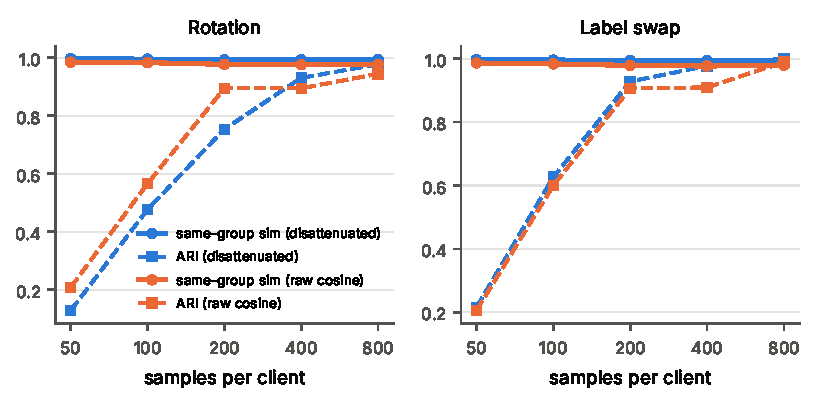
\includegraphics[width=0.85\linewidth]{sample_size.pdf}
\caption{Same-group similarity (solid) and ARI (dashed) as a function of the client size. Blue: disattenuated; orange: raw cosine.}\label{fig:size}
\end{figure}
\begin{figure}[h]
\centering
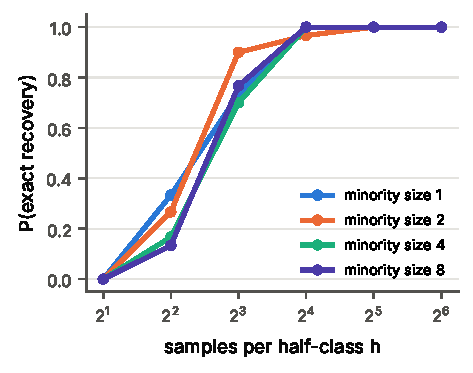
\includegraphics[width=0.45\linewidth]{theory_minority.pdf}
\caption{Synthetic validation of Corollary~\ref{cor:sc}: exact recovery of a minority group does not depend on its size.}\label{fig:thminority}
\end{figure}
\begin{table}[h]
\centering
\caption{Sensitivity to the shrinkage $\lambda$ at $\tau=0.9$: ARI / number of clusters (3 seeds, clustering step). For the label-only scenario the correct $K$ is 1. Only $\lambda=0.02$ and $0.1$ satisfy the condition of Corollary~\ref{cor:sc} when $\gamma=0.1$.}\label{tab:lambda}
\small
\begin{tabular}{lccccc}
\toprule
Scenario & $\lambda=0.02$ & $\lambda=0.1$ & $\lambda=0.2$ & $\lambda=0.5$ & $\lambda=1.0$ \\
\midrule
Rotation & 0.93 / 4.3 & 0.93 / 4.3 & 0.93 / 4.3 & 0.93 / 4.3 & 0.93 / 4.0 \\
Label swap & 0.98 / 4.0 & 0.98 / 4.0 & 0.98 / 4.0 & 0.98 / 4.0 & 0.98 / 4.0 \\
Rotation + QS & 0.92 / 5.0 & 0.92 / 5.0 & 0.91 / 5.0 & 0.98 / 4.3 & 0.98 / 4.0 \\
Mixed + QS & 0.96 / 4.0 & 0.96 / 4.0 & 0.96 / 4.0 & 0.96 / 4.0 & 0.96 / 4.0 \\
Label skew only & 1.00 / 1.0 & 1.00 / 1.0 & 1.00 / 1.0 & 1.00 / 1.0 & 1.00 / 1.0 \\
Minority groups & 1.00 / 4.0 & 0.99 / 4.3 & 0.99 / 4.3 & 0.99 / 4.0 & 1.00 / 4.0 \\
\bottomrule
\end{tabular}
\end{table}


\begin{tableorg}[!htbp]
\centering
\caption{Hierarchical comparison of DisCo-CFL with each baseline on the held-out runs only, i.e.\ excluding the development runs listed in Section~\ref{sec:setup}. Columns as in Table~\ref{tab:hier}.}\label{tab:hier_heldout}
{\scriptsize
\begin{tabular}{l c c c c c c c c c}
\toprule
Baseline & \multicolumn{3}{c}{Accuracy} & \multicolumn{3}{c}{Concept acc.} & \multicolumn{3}{c}{Worst group} \\
\cmidrule(lr){2-4}
\cmidrule(lr){5-7}
\cmidrule(lr){8-10}
 & $\Delta$ [95\% CI] & W/T/L & p & $\Delta$ [95\% CI] & W/T/L & p & $\Delta$ [95\% CI] & W/T/L & p \\
\midrule
\multicolumn{10}{l}{\textit{(a) Small-CNN benchmarks (main, other, sweep scenarios pooled)}} \\
FedAvg & +6.7 [+4.6, +9.0] & 16/3/0 & <0.001 & +11.7 [+8.1, +15.5] & 16/2/1 & <0.001 & +10.0 [+6.3, +14.2] & 16/2/1 & <0.001 \\
Local & +0.6 [$-$1.9, +2.5] & 9/0/2 & 0.160 & +20.5 [+15.9, +24.9] & 11/0/0 & <0.001 & +0.3 [$-$2.8, +2.9] & 9/0/2 & 0.160 \\
FedAvg-FT & +2.6 [+0.2, +4.5] & 9/0/2 & 0.034 & +8.7 [+6.4, +10.5] & 10/0/1 & <0.001 & +3.3 [$-$0.1, +6.0] & 9/0/2 & 0.034 \\
IFCA & +1.6 [+0.2, +2.8] & 16/1/2 & 0.010 & +7.3 [+4.7, +9.9] & 17/0/2 & <0.001 & +2.4 [+0.6, +4.0] & 17/0/2 & 0.005 \\
FeSEM & +2.9 [+1.6, +4.1] & 16/0/3 & <0.001 & +9.3 [+7.2, +11.5] & 19/0/0 & <0.001 & +4.7 [+2.8, +6.6] & 17/0/2 & <0.001 \\
MTCFL & +0.9 [$-$0.6, +2.1] & 17/0/2 & 0.007 & +12.0 [+10.7, +13.2] & 19/0/0 & <0.001 & +0.8 [$-$1.1, +2.4] & 17/0/2 & 0.009 \\
FL+HC & +1.1 [+0.3, +1.9] & 15/1/3 & 0.005 & +4.7 [+3.4, +6.1] & 18/0/1 & <0.001 & +1.4 [+0.2, +2.6] & 15/1/3 & 0.011 \\
PACFL & +3.7 [+0.9, +6.7] & 15/1/3 & 0.004 & +9.2 [+4.3, +14.4] & 17/0/2 & <0.001 & +5.7 [+1.9, +10.2] & 16/0/3 & 0.002 \\
StoCFL & +4.3 [+2.4, +6.1] & 17/0/2 & <0.001 & +14.8 [+11.6, +18.0] & 19/0/0 & <0.001 & +6.0 [+3.1, +9.2] & 17/0/2 & <0.001 \\
StoCFL-W & +2.1 [+0.8, +3.2] & 16/0/3 & 0.004 & +10.5 [+8.7, +12.3] & 19/0/0 & <0.001 & +2.5 [+0.8, +4.0] & 16/0/3 & 0.005 \\
FedCCFA & +2.8 [+0.9, +4.3] & 17/0/2 & 0.001 & +10.3 [+8.1, +12.2] & 18/0/1 & <0.001 & +4.0 [+1.3, +6.3] & 17/0/2 & <0.001 \\
FedDAG-C & +2.0 [+0.7, +3.3] & 15/0/4 & 0.003 & +7.5 [+4.8, +10.5] & 19/0/0 & <0.001 & +3.2 [+1.3, +5.2] & 15/1/3 & 0.001 \\
\addlinespace
\multicolumn{10}{l}{\textit{(b) Realistic benchmarks}} \\
FedAvg & +1.4 [$-$0.3, +3.0] & 4/0/1 & 0.094 & +2.0 [$-$0.6, +4.4] & 3/0/2 & 0.156 & +1.4 [$-$1.2, +3.9] & 3/0/2 & 0.156 \\
Local & +9.4 [+5.3, +13.5] & 5/0/0 & 0.031 & +31.1 [+28.1, +33.8] & 5/0/0 & 0.031 & +9.7 [+5.8, +13.7] & 5/0/0 & 0.031 \\
FedAvg-FT & +6.9 [+4.6, +9.9] & 5/0/0 & 0.031 & +7.3 [+3.5, +11.2] & 5/0/0 & 0.031 & +9.4 [+3.7, +15.9] & 5/0/0 & 0.031 \\
IFCA & +3.6 [+2.1, +6.0] & 5/0/0 & 0.031 & +7.8 [+5.8, +9.9] & 5/0/0 & 0.031 & +3.8 [+1.0, +6.6] & 4/0/1 & 0.062 \\
FeSEM & +2.6 [+1.4, +4.1] & 5/0/0 & 0.031 & +5.4 [+3.3, +7.4] & 5/0/0 & 0.031 & +2.9 [+0.5, +5.2] & 4/0/1 & 0.062 \\
MTCFL & +3.7 [+1.8, +5.7] & 5/0/0 & 0.031 & +14.1 [+12.7, +15.4] & 5/0/0 & 0.031 & +3.8 [+1.2, +6.2] & 5/0/0 & 0.031 \\
FL+HC & +1.5 [+0.3, +2.5] & 4/0/1 & 0.062 & +3.7 [+0.4, +6.8] & 4/0/1 & 0.062 & +2.4 [+0.5, +4.2] & 5/0/0 & 0.031 \\
PACFL & +1.9 [+0.2, +4.2] & 4/0/1 & 0.094 & +3.9 [+1.4, +6.4] & 4/1/0 & 0.062 & +1.7 [$-$1.5, +4.9] & 4/0/1 & 0.219 \\
StoCFL & +3.2 [+0.9, +5.4] & 4/0/1 & 0.062 & +12.7 [+3.5, +22.7] & 4/0/1 & 0.062 & +3.4 [+1.2, +5.5] & 4/0/1 & 0.062 \\
StoCFL-W & +4.8 [+2.3, +7.4] & 5/0/0 & 0.031 & +17.4 [+12.5, +22.4] & 5/0/0 & 0.031 & +4.8 [+1.4, +8.1] & 5/0/0 & 0.031 \\
FedCCFA & +2.4 [+1.8, +3.1] & 5/0/0 & 0.031 & +4.1 [+1.5, +6.7] & 5/0/0 & 0.031 & +3.0 [+1.3, +4.3] & 5/0/0 & 0.031 \\
FedDAG-C & +3.0 [+1.6, +4.7] & 5/0/0 & 0.031 & +7.5 [+4.3, +11.0] & 5/0/0 & 0.031 & +3.9 [+1.9, +6.3] & 5/0/0 & 0.031 \\
\addlinespace
\multicolumn{10}{l}{\textit{(c) Additional pre-registered benchmarks}} \\
FedAvg & +10.7 [+5.6, +15.6] & 7/0/0 & 0.008 & +17.5 [+8.5, +25.8] & 6/0/1 & 0.023 & +12.9 [+6.8, +18.5] & 7/0/0 & 0.008 \\
Local & +6.1 [+3.6, +8.3] & 6/0/1 & 0.016 & +27.9 [+19.1, +34.3] & 7/0/0 & 0.008 & +6.2 [+2.5, +9.0] & 6/0/1 & 0.016 \\
FedAvg-FT & +6.3 [+3.1, +10.0] & 6/0/1 & 0.016 & +14.0 [+8.0, +20.1] & 7/0/0 & 0.008 & +7.1 [+2.7, +11.5] & 6/0/1 & 0.016 \\
IFCA & +3.7 [+1.9, +5.7] & 7/0/0 & 0.008 & +9.6 [+5.1, +14.2] & 7/0/0 & 0.008 & +5.4 [+2.3, +8.6] & 7/0/0 & 0.008 \\
FeSEM & +4.1 [+2.3, +6.3] & 7/0/0 & 0.008 & +10.7 [+6.0, +15.5] & 7/0/0 & 0.008 & +5.5 [+2.6, +8.8] & 7/0/0 & 0.008 \\
MTCFL & +3.1 [+1.2, +4.9] & 6/0/1 & 0.016 & +15.2 [+8.8, +20.6] & 7/0/0 & 0.008 & +2.9 [$-$0.1, +5.1] & 6/0/1 & 0.078 \\
FL+HC & +1.2 [+0.3, +2.1] & 6/0/1 & 0.016 & +4.0 [+1.2, +7.3] & 6/0/1 & 0.023 & +1.2 [$-$0.8, +2.9] & 4/0/3 & 0.109 \\
PACFL & +6.9 [+2.8, +11.5] & 5/0/1 & 0.031 & +13.9 [+5.5, +22.4] & 5/0/1 & 0.031 & +8.7 [+3.3, +14.7] & 5/0/1 & 0.031 \\
StoCFL & +7.6 [+5.0, +10.3] & 7/0/0 & 0.008 & +22.1 [+15.8, +28.0] & 7/0/0 & 0.008 & +8.8 [+5.2, +12.6] & 7/0/0 & 0.008 \\
StoCFL-W & +4.3 [+2.3, +6.4] & 7/0/0 & 0.008 & +16.6 [+10.1, +23.3] & 7/0/0 & 0.008 & +4.7 [+1.4, +7.5] & 6/0/1 & 0.023 \\
FedCCFA & +4.3 [+1.0, +8.2] & 6/0/1 & 0.039 & +12.4 [+5.4, +19.8] & 6/0/1 & 0.016 & +4.3 [+0.2, +8.6] & 6/0/1 & 0.055 \\
FedDAG-C & +4.5 [+1.5, +9.0] & 6/0/0 & 0.016 & +9.6 [+3.2, +17.1] & 6/0/0 & 0.016 & +6.8 [+2.4, +13.0] & 6/0/0 & 0.016 \\
\bottomrule
\end{tabular}
}

\end{tableorg}

\begin{tableorg}[!htbp]
\centering
\caption{Failure rates per dataset (\%): fraction of runs with ARI below $0.5$ in the scenarios with more than one group. FMNIST: Fashion-MNIST, including the robustness sweeps; (R): pretrained ResNet-18. Runs per cell: 10 per dataset with two scenarios (5 seeds each), 5 for Office-Home and AG News, and 49 for Fashion-MNIST (five main scenarios with 5 seeds, eight sweeps with 3; 25 for DisCo-noAttach, which is not run on the sweeps). ``--'': not run (PACFL and FedDAG-C need image inputs).}\label{tab:failure_ds}
{\scriptsize
\resizebox{\textwidth}{!}{%
\begin{tabular}{l c c c c c c c c c c c}
\toprule
Method & FMNIST & MNIST & KMNIST & EMNIST & SVHN & CIFAR-10 & PACS & Office-Home & CIFAR-100 (R) & CIFAR-10 (R) & AG News \\
\midrule
DisCo & 2 & 0 & 0 & 30 & 100 & 100 & 0 & 100 & 50 & 50 & 0 \\
DisCo-noAttach & 0 & 0 & 0 & 40 & 100 & 100 & 0 & 100 & 50 & 50 & 0 \\
IFCA & 80 & 40 & 80 & 80 & 100 & 100 & 90 & 100 & 100 & 80 & 20 \\
FeSEM & 84 & 70 & 70 & 60 & 100 & 100 & 100 & 100 & 100 & 90 & 100 \\
MTCFL & 100 & 100 & 100 & 100 & 100 & 100 & 100 & 100 & 100 & 100 & 100 \\
FL+HC & 37 & 20 & 30 & 50 & 100 & 100 & 100 & 20 & 70 & 60 & 100 \\
PACFL & 71 & 90 & 100 & 70 & 100 & 100 & 90 & 100 & 90 & 100 & -- \\
StoCFL & 100 & 100 & 100 & 100 & 100 & 100 & 100 & 100 & 100 & 100 & 100 \\
StoCFL-W & 100 & 100 & 100 & 100 & 100 & 100 & 100 & 100 & 100 & 100 & 100 \\
FedCCFA & 100 & 100 & 100 & 100 & 100 & 100 & 100 & 100 & 100 & 100 & 60 \\
FedDAG-C & 57 & 60 & 50 & 50 & 100 & 100 & 100 & 100 & 100 & 100 & -- \\
\bottomrule
\end{tabular}}
}

\end{tableorg}


\subsection{Further experimental results}\label{app:more}

\paragraph{Edge cases.} Table~\ref{tab:edge} varies the minimum class size $m$ in three federations. The default $m=4$ is best or close to best. A larger $m$ discards classes and hence evidence, and the effect is strongest with small clients ($m=16$: ARI $0.28$, 30\% of the conflicting pairs merged), because clients then report few classes and share few discriminative ones. With extreme label skew ($\alpha=0.1$) and with small clients, ARI falls to $0.71$ and $0.66$ at the default, with 3.5\% and 9.3\% conflicting merges. Under extreme label skew these are the coverage failures anticipated in Remark~\ref{rem:scope}(d); with small clients the main cause is the smaller separation at a reference model trained on less data, as in the sample-size study. The table averages the four scenarios, including the label-only one, which explains $K<4$ for the default federation. The reliability floor $r_{\min}$ has no measurable effect between $0$ and $0.2$: over the 144 combinations of scenario, federation, seed and $m$, changing $r_{\min}$ changes ARI by at most $0.017$.

\begin{table}[!htbp]
\centering
\caption{Edge cases: minimum class size $m$ in three federations (Rotation, Label swap, \emph{Mixed + QS} and label-only scenarios, 3 seeds, $r_{\min}=0.02$).}\label{tab:edge}
\scriptsize
\setlength{\tabcolsep}{4pt}
\begin{tabular}{llcccc}
\toprule
Federation & $m$ & ARI & Conflict\% & $K$ & Low-evidence clients \\
\midrule
Default federation & 2 & 0.86 & 0.3 & 4.0 & 0.0 \\
 & 4 & 0.97 & 0.2 & 3.3 & 0.0 \\
 & 8 & 0.91 & 1.5 & 3.3 & 0.0 \\
 & 16 & 0.75 & 5.0 & 3.8 & 0.2 \\
\midrule
Extreme label skew ($\alpha=0.1$) & 2 & 0.72 & 3.1 & 3.5 & 0.0 \\
 & 4 & 0.71 & 3.5 & 3.7 & 0.0 \\
 & 8 & 0.64 & 6.0 & 3.8 & 0.0 \\
 & 16 & 0.61 & 8.7 & 3.7 & 0.0 \\
\midrule
Small clients (100 samples) & 2 & 0.66 & 6.1 & 3.9 & 0.0 \\
 & 4 & 0.66 & 9.3 & 3.2 & 0.0 \\
 & 8 & 0.55 & 15.0 & 3.2 & 0.0 \\
 & 16 & 0.28 & 30.1 & 2.9 & 2.4 \\
\bottomrule
\end{tabular}

\end{table}



\paragraph{Theory in practice.}
Figure~\ref{fig:theory} validates the theory on synthetic signatures with known ground truth ($p=512$, noise of effective rank 16). The disattenuated similarity is nearly unbiased for every half size $h$, whereas the raw cosine is biased by up to $-0.37$. Safety and maximality are reached with probability 1 once $h\ge64$ for all separations $\Delta\in[0.2,0.7]$, and exact recovery is reached under full class support. The required $h$ grows as $\Delta$ shrinks. Recovery of a minority group of 1, 2, 4 or 8 clients follows the same curve (Figure~\ref{fig:thminority} in Appendix~\ref{app:figs}), as Corollary~\ref{cor:sc} states.

\begin{figure}[!htbp]
\centering
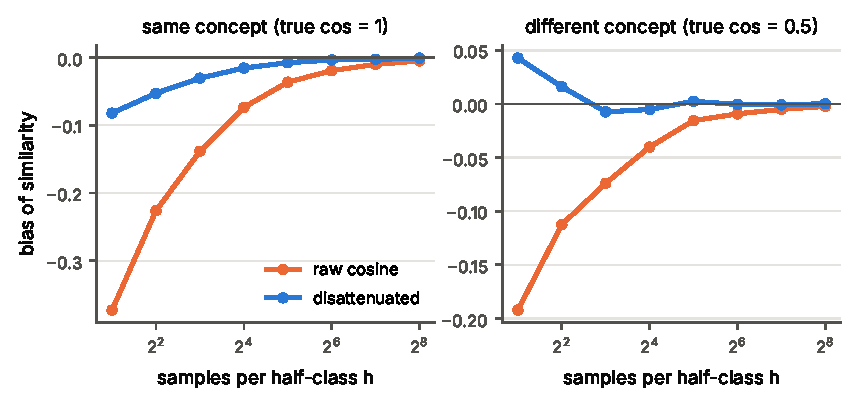
\includegraphics[width=0.49\linewidth]{theory_estimation.pdf}\hfill
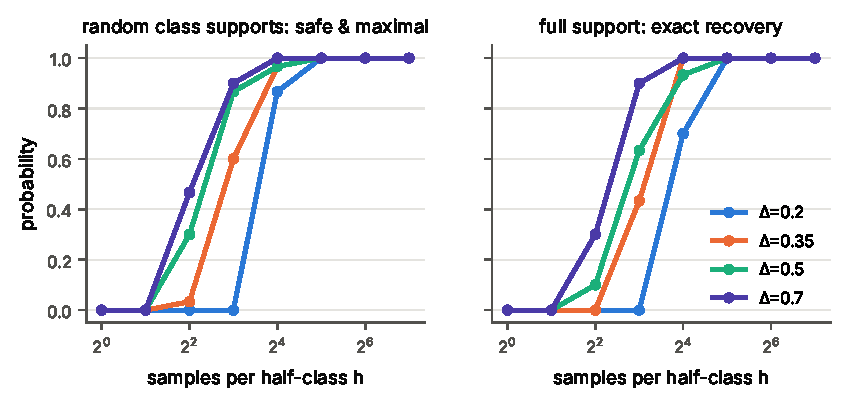
\includegraphics[width=0.49\linewidth]{theory_recovery.pdf}
\caption{Synthetic validation. Left: bias of the similarity estimate. Right: probability of the guarantees of Theorem~\ref{thm:rec}.}\label{fig:theory}
\end{figure}



\begin{tableorg}[!htbp]
\centering
\caption{Class-support disclosure under DP (rotation and label swap, 3 seeds). Plain: only the held classes are reported. Padded: noise vectors are sent for the other classes. Support acc.: accuracy of the server's guess ``class held iff $R_i^c>0$''; FPR: rate at which padded classes are guessed as held.}\label{tab:support}
\scriptsize
\setlength{\tabcolsep}{3pt}
\resizebox{\textwidth}{!}{%
\begin{tabular}{cccccccc}
\toprule
$\sigma$ & Samples/client & $\varepsilon$ & ARI plain & ARI padded & Support acc.\ plain (\%) & Support acc.\ padded (\%) & Support FPR padded (\%) \\
\midrule
0.5 & 400 & 10.00 & 0.43 & 0.26 & 91.3 & 77.2 & 38.1 \\
0.5 & 1500 & 10.00 & 0.75 & 0.45 & 92.2 & 83.9 & 35.3 \\
1 & 400 & 4.38 & 0.26 & 0.15 & 84.4 & 70.2 & 38.1 \\
1 & 1500 & 4.38 & 0.62 & 0.40 & 87.6 & 79.3 & 35.3 \\
2 & 400 & 1.99 & 0.08 & 0.10 & 77.0 & 62.9 & 38.1 \\
2 & 1500 & 1.99 & 0.48 & 0.32 & 81.7 & 73.3 & 35.3 \\
\bottomrule
\end{tabular}}

\end{tableorg}

\begin{table}[!htbp]
\centering
\caption{Concept drift after clustering (Fashion-MNIST, 3 seeds): detection rate of drifted clients, false-alarm rate on unchanged clients, and share of drifted clients reassigned to the cluster of their new group.}\label{tab:drift}
\scriptsize
\setlength{\tabcolsep}{4pt}
\begin{tabular}{llccc}
\toprule
Scenario & $q$ & Detection (\%) & False alarm (\%) & Reassigned correctly (\%) \\
\midrule
Rotation & 0.1 & 100.0 & 30.6 & 75.0 \\
Rotation & 0.2 & 100.0 & 59.4 & 54.2 \\
\midrule
Label swap & 0.1 & 100.0 & 45.4 & 66.7 \\
Label swap & 0.2 & 100.0 & 66.7 & 37.5 \\
\bottomrule
\end{tabular}

\end{table}

\begin{tableorg}[!htbp]
\centering
\caption{The complete pipeline with the default shrinkage $\lambda=0.5$ and with $\lambda=0.02$, for which the evidence condition of Theorem~\ref{thm:rec} can hold (Remark~\ref{rem:scope}(e)); all small-CNN scenarios (5 seeds; sweeps 3 seeds). $\Delta$: difference in mean accuracy (points). FMNIST: Fashion-MNIST; QS: quantity skew; part.: participation.}\label{tab:l02}
\scriptsize
\setlength{\tabcolsep}{3pt}
\resizebox{\textwidth}{!}{%
\begin{tabular}{lrccccccc}
\toprule
 & & \multicolumn{3}{c}{Accuracy (\%)} & \multicolumn{2}{c}{ARI} & \multicolumn{2}{c}{$K$} \\
\cmidrule(lr){3-5}\cmidrule(lr){6-7}\cmidrule(lr){8-9}
Scenario & $n$ & $\lambda=0.5$ & $\lambda=0.02$ & $\Delta$ & $\lambda=0.5$ & $\lambda=0.02$ & $\lambda=0.5$ & $\lambda=0.02$ \\
\midrule
FMNIST rotation & 5 & 89.1 & 89.1 & -0.0 & 0.92 & 0.92 & 4.4 & 4.4 \\
FMNIST label swap & 5 & 89.2 & 89.2 & -0.0 & 0.97 & 0.97 & 4.0 & 4.2 \\
FMNIST rotation + QS & 5 & 88.9 & 88.7 & -0.2 & 0.99 & 0.94 & 4.2 & 4.8 \\
FMNIST mixed + QS & 5 & 89.0 & 89.0 & +0.1 & 0.96 & 0.96 & 4.2 & 4.2 \\
FMNIST label skew only & 5 & 94.5 & 94.5 & -0.0 & 1.00 & 1.00 & 1.0 & 1.0 \\
FMNIST minority & 5 & 89.2 & 89.3 & +0.0 & 0.99 & 1.00 & 4.0 & 4.0 \\
MNIST rotation & 5 & 98.1 & 98.1 & -0.0 & 1.00 & 1.00 & 4.0 & 4.0 \\
MNIST label swap & 5 & 98.0 & 98.0 & +0.0 & 0.99 & 0.99 & 4.0 & 4.0 \\
KMNIST rotation & 5 & 86.9 & 87.1 & +0.2 & 0.96 & 0.98 & 4.2 & 4.2 \\
KMNIST label swap & 5 & 87.3 & 87.3 & +0.0 & 0.95 & 0.97 & 4.2 & 4.0 \\
EMNIST rotation & 5 & 84.2 & 83.8 & -0.3 & 0.98 & 0.95 & 4.4 & 4.6 \\
EMNIST label swap & 5 & 83.7 & 83.3 & -0.4 & 0.56 & 0.56 & 5.6 & 6.2 \\
SVHN rotation & 5 & 69.3 & 69.3 & +0.0 & 0.00 & 0.00 & 1.0 & 1.0 \\
SVHN label swap & 5 & 73.3 & 73.3 & +0.0 & 0.00 & 0.00 & 1.0 & 1.0 \\
CIFAR-10 rotation & 5 & 63.5 & 63.6 & +0.1 & 0.01 & 0.02 & 1.4 & 1.4 \\
CIFAR-10 label swap & 5 & 65.3 & 65.2 & -0.0 & 0.28 & 0.27 & 2.4 & 2.4 \\
Rotation $15^\circ$ & 3 & 88.7 & 88.5 & -0.2 & 0.52 & 0.44 & 2.7 & 2.7 \\
Rotation $30^\circ$ & 3 & 88.8 & 89.1 & +0.2 & 0.93 & 0.98 & 4.0 & 4.0 \\
Rotation $45^\circ$ & 3 & 89.1 & 89.1 & +0.0 & 1.00 & 1.00 & 4.0 & 4.0 \\
2 label permutations & 3 & 89.5 & 89.5 & -0.0 & 1.00 & 1.00 & 2.0 & 2.0 \\
8 label permutations & 3 & 88.2 & 88.2 & +0.1 & 0.79 & 0.81 & 8.7 & 8.7 \\
Rotation, 30\% part. & 3 & 87.1 & 87.0 & -0.0 & 0.93 & 0.98 & 4.3 & 4.0 \\
Label swap, 30\% part. & 3 & 87.3 & 87.3 & -0.1 & 0.98 & 0.98 & 4.0 & 4.0 \\
Rotation, 200 clients & 3 & 86.5 & 86.5 & +0.0 & 0.88 & 0.89 & 4.7 & 4.7 \\
\bottomrule
\end{tabular}}

\end{tableorg}

\begin{tableorg}[!htbp]
\centering
\caption{Dependence on the reference model (3 seeds). The reference model is trained for 10 rounds on all clients, on a random half of them, or on all clients except those of group 0; all clients are then clustered at that model. ARI (in/out): ARI among the clients that did and did not train the reference model. Merge g0: conflict-merge rate of the pairs that involve group 0. FMNIST: Fashion-MNIST; QS: quantity skew.}\label{tab:refmodel}
\scriptsize
\setlength{\tabcolsep}{3pt}
\resizebox{\textwidth}{!}{%
\begin{tabular}{lcccccccc}
\toprule
 & All clients & \multicolumn{4}{c}{Random half} & \multicolumn{3}{c}{Without group 0} \\
\cmidrule(lr){2-2}\cmidrule(lr){3-6}\cmidrule(lr){7-9}
Scenario & ARI & ARI & ARI (in) & ARI (out) & $K$ & ARI & $K$ & Merge g0 (\%) \\
\midrule
FMNIST rotation & 0.93 & 0.98 & 1.00 & 0.94 & 4.00 & 0.98 & 4.00 & 1.1 \\
FMNIST label swap & 0.98 & 0.98 & 1.00 & 0.95 & 4.00 & 0.98 & 4.00 & 0.0 \\
FMNIST mixed + QS & 0.96 & 0.93 & 1.00 & 0.91 & 4.00 & 0.96 & 4.00 & 0.0 \\
FMNIST label skew only & 1.00 & 1.00 & 1.00 & 1.00 & 1.00 & -- & -- & -- \\
MNIST rotation & 1.00 & 1.00 & 1.00 & 1.00 & 4.00 & 1.00 & 4.00 & 0.0 \\
MNIST label swap & 1.00 & 1.00 & 1.00 & 1.00 & 4.00 & 1.00 & 4.00 & 0.0 \\
\bottomrule
\end{tabular}}

\end{tableorg}

\begin{tableorg}[!htbp]
\centering
\caption{Calibration of the certificate standard errors on synthetic signatures (200 draws per setting; median over the 12 settings of cluster size $M\in\{3,6,12\}$ and number of classes $C\in\{2,5,10,20\}$ for each case and half size $h$). SD/se: standard deviation of $s_{iM}$ over draws divided by the mean standard error. Bias/se: mean error in units of the mean standard error. Coverage: fraction of draws whose $\pm2\,\mathrm{se}$ interval contains the population value, before and after removing the mean bias.}\label{tab:certgrid}
\scriptsize
\resizebox{\textwidth}{!}{%
\begin{tabular}{lrcccc}
\toprule
Case & $h$ & SD/se, median [range] & Bias / se & Coverage (\%) & Debiased coverage (\%) \\
\midrule
Same concept & 10 & 0.94 [0.86, 1.08] & -2.52 & 30 & 89 \\
 & 20 & 0.92 [0.80, 1.06] & -2.51 & 32 & 88 \\
 & 50 & 0.94 [0.81, 1.09] & -2.53 & 29 & 88 \\
 & 200 & 0.92 [0.84, 1.03] & -2.58 & 29 & 89 \\
Different, $\Delta=0.1$ & 10 & 1.09 [1.00, 1.22] & +0.20 & 81 & 81 \\
 & 20 & 1.13 [0.98, 1.27] & +0.13 & 80 & 82 \\
 & 50 & 1.16 [1.03, 1.23] & +0.10 & 80 & 80 \\
 & 200 & 1.13 [1.06, 1.46] & +0.10 & 80 & 80 \\
Different, $\Delta=0.3$ & 10 & 1.13 [1.01, 1.43] & +0.31 & 78 & 80 \\
 & 20 & 1.18 [1.13, 1.30] & +0.25 & 78 & 80 \\
 & 50 & 1.16 [1.06, 1.20] & +0.17 & 81 & 80 \\
 & 200 & 1.17 [1.04, 1.26] & +0.13 & 79 & 79 \\
\bottomrule
\end{tabular}}

\end{tableorg}

\begin{table}[!htbp]
\centering
\caption{Malicious clients (Fashion-MNIST rotation and label swap, 3 seeds each): ARI and conflict-merge rate among the honest clients, and the fate of the malicious clients (mean counts: isolated in a singleton, flagged as low-evidence or anomalous, merged into an honest cluster, or grouped only with other malicious clients).}\label{tab:byz}
\scriptsize
\setlength{\tabcolsep}{4pt}
\begin{tabular}{llcccccc}
\toprule
Attack & $m$ & Honest ARI & Honest conflict\% & Isolated & Flagged & Merged & Other \\
\midrule
Random vectors & 1 & 0.95 & 0.4 & 0.33 & 0.67 & 0.00 & 0.00 \\
 & 2 & 0.95 & 0.4 & 0.00 & 2.00 & 0.00 & 0.00 \\
 & 4 & 0.96 & 0.1 & 0.00 & 4.00 & 0.00 & 0.00 \\
\midrule
Mimicry & 1 & 0.99 & 0.3 & 0.00 & 0.00 & 1.00 & 0.00 \\
 & 2 & 0.94 & 0.7 & 0.00 & 0.00 & 2.00 & 0.00 \\
 & 4 & 0.97 & 0.1 & 0.00 & 0.00 & 4.00 & 0.00 \\
\midrule
Sign flip & 1 & 0.95 & 0.4 & 1.00 & 0.00 & 0.00 & 0.00 \\
 & 2 & 0.95 & 0.4 & 1.67 & 0.00 & 0.00 & 0.33 \\
 & 4 & 0.96 & 0.1 & 1.67 & 0.00 & 0.00 & 2.33 \\
\bottomrule
\end{tabular}

\end{table}

\begin{tableorg}[!htbp]
\centering
\caption{Attempted remedies for the failures: full-layer signature and 30 warm-up rounds (3 seeds).}\label{tab:real_variants}
\scriptsize
\begin{tabular}{lccccc}
\toprule
Method & Acc & Concept & ARI & $K$ & Conflict\% \\
\midrule
\multicolumn{6}{l}{\textit{Office-Home (4 domains, 65 classes)}}\\
FedAvg & 68.7 & 58.1 & 0.00 & 1.0 & 100.0 \\
FeSEM & 68.1 & 54.6 & 0.05 & 4.0 & 37.7 \\
Oracle & 70.5 & 61.4 & 1.00 & 4.0 & 0.0 \\
DisCo-CFL (default) & 69.4 & 58.1 & 0.32 & 3.3 & 29.1 \\
DisCo-CFL, full-layer signature & 70.0 & 59.7 & 0.75 & 4.7 & 6.7 \\
DisCo-CFL, 30 warm-up rounds & 70.0 & 59.5 & 0.41 & 4.3 & 19.1 \\
\midrule
\multicolumn{6}{l}{\textit{CIFAR-100, rotations}}\\
FedAvg & 52.8 & 42.2 & 0.00 & 1.0 & 100.0 \\
FeSEM & 49.1 & 37.3 & -0.01 & 4.0 & 31.3 \\
Oracle & 51.7 & 41.3 & 1.00 & 4.0 & 0.0 \\
DisCo-CFL (default) & 50.8 & 39.7 & 0.06 & 3.0 & 56.3 \\
DisCo-CFL, full-layer signature & 50.8 & 39.9 & 0.32 & 3.7 & 27.8 \\
DisCo-CFL, 30 warm-up rounds & 52.2 & 41.4 & 0.01 & 2.3 & 71.0 \\
\bottomrule
\end{tabular}

\end{tableorg}

\begin{tableorg}[!htbp]
\centering
\caption{Ablation on CIFAR-100 with label-swap groups (3 seeds). Columns as in Table~\ref{tab:real_variants}.}\label{tab:real_ablation}
\scriptsize
\begin{tabular}{lccccc}
\toprule
Variant & Acc & Concept & ARI & $K$ & Conflict\% \\
\midrule
DisCo-CFL (full) & 57.7 & 46.5 & 0.93 & 4 & 1.5 \\
no attachment stage & 57.2 & 45.6 & 0.90 & 5 & 1.3 \\
\bottomrule
\end{tabular}

\end{tableorg}

\paragraph{Robustness sweeps.}
Table~\ref{tab:sweeps} varies one factor at a time on Fashion-MNIST: the strength of the concept shift, the number of groups, the fraction of participating clients and the number of clients. Baselines are given the true $K$ where they need it.

\begin{tableorg}[!htbp]
\centering
\caption{Robustness sweeps (Fashion-MNIST, 3 seeds; the $90^\circ$ row repeats the \emph{Rotation} scenario with 5 seeds). For DisCo-CFL: ARI, number of clusters, conflict-merge rate, accuracy and concept accuracy. For comparison: the best baseline on accuracy and on concept accuracy (in parentheses), and the Oracle's accuracy.}\label{tab:sweeps}
\scriptsize
\setlength{\tabcolsep}{3pt}
\resizebox{\textwidth}{!}{%
\begin{tabular}{llcccccccc}
\toprule
& & \multicolumn{5}{c}{DisCo-CFL} & & & \\
\cmidrule(lr){3-7}
Factor & Setting & ARI & $K$ & Conflict\% & Acc & Concept & Best baseline Acc & Best baseline Concept & Oracle Acc \\
\midrule
Strength & $\theta=15^\circ$ & 0.52 & 2.7 & 30.0 & 88.7 & 76.0 & 88.7 (PACFL) & 75.1 (PACFL) & 89.3 \\
Strength & $\theta=30^\circ$ & 0.93 & 4.0 & 1.7 & 88.8 & 76.3 & 88.3 (FedDAG-C) & 74.5 (PACFL) & 89.1 \\
Strength & $\theta=45^\circ$ & 1.00 & 4.0 & 0.0 & 89.1 & 77.0 & 89.3 (FedDAG-C) & 76.6 (FedDAG-C) & 89.2 \\
Strength & $\theta=90^\circ$ & 0.92 & 4.4 & 1.1 & 89.1 & 76.4 & 88.6 (FedDAG-C) & 74.3 (FL+HC) & 89.3 \\
Groups & $K=2$ & 1.00 & 2.0 & 0.0 & 89.5 & 78.2 & 89.3 (FL+HC) & 77.3 (FL+HC) & 89.5 \\
Groups & $K=4$ & 0.97 & 4.0 & 0.0 & 89.2 & 76.7 & 88.3 (FL+HC) & 72.6 (FL+HC) & 89.2 \\
Groups & $K=8$ & 0.79 & 8.7 & 1.7 & 88.2 & 70.7 & 87.2 (MTCFL) & 59.8 (MTCFL) & 88.6 \\
Participation 30\% & rotation & 0.93 & 4.3 & 0.8 & 87.1 & 72.3 & 86.9 (FedDAG-C) & 70.0 (FedDAG-C) & 87.2 \\
Participation 30\% & label swap & 0.98 & 4.0 & 0.0 & 87.3 & 73.1 & 85.7 (FedCCFA) & 66.4 (FL+HC) & 87.2 \\
Scale & $N=200$ & 0.88 & 4.7 & 2.9 & 86.5 & 73.1 & 85.2 (IFCA) & 70.6 (FedDAG-C) & 87.2 \\
\bottomrule
\end{tabular}}

\end{tableorg}

\paragraph{Strength of the shift.} With rotations of $0,\theta,2\theta,3\theta$ degrees, DisCo-CFL separates the groups perfectly at $\theta=45^\circ$ (ARI $1.00$) and almost perfectly at $30^\circ$ (ARI $0.93$). At $15^\circ$ neighbouring concepts are so close that their class-conditional gradients agree above the threshold: the estimated separation is $\hat\Delta=0.06$, below $1-\tau=0.1$ (Table~\ref{tab:diag}), and DisCo-CFL merges them (ARI $0.52$, $K=2.7$). This is what the separation assumption predicts: the method groups what it cannot tell apart, and the diagnostic shows it. It costs little, because nearby concepts can share a model: accuracy is 88.7\% against 89.3\% for the Oracle, equal to the best baseline (PACFL, given $K$). For $\theta\ge30^\circ$ DisCo-CFL is within $0.3$ points of the Oracle; at $45^\circ$ FedDAG-C is $0.2$ points more accurate.

\paragraph{Number of groups.} With $K=2$, $4$ and $8$ label-permutation groups, DisCo-CFL finds the number of groups without being told (2.0, 4.0 and 8.7 clusters). With $K=8$, recovery is incomplete (ARI $0.79$, 1.7\% of the conflicting pairs merged): with Dirichlet label skew, many clients hold few of the classes that distinguish two of the eight permutations, so coverage is weaker. Accuracy is within $0.4$ points of the Oracle for all $K$, and $0.2$--$1.0$ points above the best baseline; concept accuracy is $0.9$--$10.9$ points above the best baseline.

\paragraph{Partial participation.} When only 30\% of the clients take part in each round, the warm-up model is noisier. DisCo-CFL still recovers the groups (ARI $0.93$ and $0.98$) and matches the Oracle within $0.1$ points, $0.2$--$1.6$ points above the best baseline in accuracy and $2.3$--$6.7$ points in concept accuracy.

\paragraph{Number of clients.} With 200 clients of 200 samples each, DisCo-CFL reaches ARI $0.88$ with 2.9\% of the conflicting pairs merged. Accuracy is 86.5\% against 87.2\% for the Oracle and 85.2\% for the best baseline (IFCA, given $K$); concept accuracy is $2.5$ points above the best baseline.

\begin{tableorg}[!htbp]
\centering
\caption{Failure rates per dataset (\%): fraction of runs with ARI below $0.5$ in the scenarios with more than one group. FMNIST: Fashion-MNIST, including the robustness sweeps; (R): pretrained ResNet-18. Runs per cell: 10 per dataset with two scenarios (5 seeds each), 5 for Office-Home and AG News, and 49 for Fashion-MNIST (five main scenarios with 5 seeds, eight sweeps with 3; 25 for DisCo-noAttach, which is not run on the sweeps). ``--'': not run (PACFL and FedDAG-C need image inputs).}\label{tab:failure_ds}
{\scriptsize
\resizebox{\textwidth}{!}{%
\begin{tabular}{l c c c c c c c c c c c}
\toprule
Method & FMNIST & MNIST & KMNIST & EMNIST & SVHN & CIFAR-10 & PACS & Office-Home & CIFAR-100 (R) & CIFAR-10 (R) & AG News \\
\midrule
DisCo & 2 & 0 & 0 & 30 & 100 & 100 & 0 & 100 & 50 & 50 & 0 \\
DisCo-noAttach & 0 & 0 & 0 & 40 & 100 & 100 & 0 & 100 & 50 & 50 & 0 \\
IFCA & 80 & 40 & 80 & 80 & 100 & 100 & 90 & 100 & 100 & 80 & 20 \\
FeSEM & 84 & 70 & 70 & 60 & 100 & 100 & 100 & 100 & 100 & 90 & 100 \\
MTCFL & 100 & 100 & 100 & 100 & 100 & 100 & 100 & 100 & 100 & 100 & 100 \\
FL+HC & 37 & 20 & 30 & 50 & 100 & 100 & 100 & 20 & 70 & 60 & 100 \\
PACFL & 71 & 90 & 100 & 70 & 100 & 100 & 90 & 100 & 90 & 100 & -- \\
StoCFL & 100 & 100 & 100 & 100 & 100 & 100 & 100 & 100 & 100 & 100 & 100 \\
StoCFL-W & 100 & 100 & 100 & 100 & 100 & 100 & 100 & 100 & 100 & 100 & 100 \\
FedCCFA & 100 & 100 & 100 & 100 & 100 & 100 & 100 & 100 & 100 & 100 & 60 \\
FedDAG-C & 57 & 60 & 50 & 50 & 100 & 100 & 100 & 100 & 100 & 100 & -- \\
\bottomrule
\end{tabular}}
}

\end{tableorg}



\end{appendices}

\end{document}
